\chapter{Temporary Muon Spectrometer}
\label{ch:tms}



%%%%%%%%%%%%%%%%%%%%%%%%%%%%%%%%
\section{Overview of the \dshort{tms}}
\label{sec:tms-ovvw}

%%%%%%%%%%%%%%%
\subsection{Introduction and Scope}
\label{sec:tms-ovvw-intro}

The \dword{dune} Collaboration's goal is to have a gaseous argon \dword{tpc} (\dword{ndgar}) immediately downstream of \dword{ndlar}, to measure the momenta of muons exiting the \dword{tpc}, as well as to study neutrino-argon interactions in more detail. This is foreseen to be primarily a non-US contribution, and is presently not on a timescale guaranteed to be ready when \dword{dune} operations to begin. The {tms} is therefore intended to operate for the early part of the running when beam intenmsities are at their lowest and \dword{dune} is not systematics limited.

This instrument is designed to have very low technical risk, be inexpensive, and have a well-understood construction time, to allow maximum flexibility to take advantage of positive developments on the international front. To that end, we intend to advance a mechanical design to the point where the go/no-go decision date is well-understood, but to defer the full electronics design until we are closer to that point, lest we do a detailed design around components that will have become obsolete.

%%%%%%%%%%%%%%%Not in Tim's new organization
\subsection{Principle of Operation}
\label{sec:tms-ovvw-op}
\fixme{Do you mean ArgonCube or the ND-LAr? It's best to have one standard name for everything. The LArTPC is ND-LAr, I think. (Anne). If you don't want us to use ArgonCube, it should not be a Dune Word. Oe better, it should write ND-LAr when we use the ArgonCube dword }

The \dword{tms} is a magnetized steel range stack between \dword{arcube} and \dword{sand}.  The face is the same size as \dword{arcube} and the depth is \SI{7}{\m}.  It consists of four columns of scintillator modules and three columns of steel; each row is \num{100} layers, with each layer containing \num{192} scintillator strips in modules of \num{48}. Panels are tilted $\pm 3^{\circ}$ in alternating U and V views. The purpose of the Muon Spectrometer is to measure the charge and momentum of muons that exit \dword{arcube} with a momentum precision comparable to the Far Detector (taken to be 4\%) in the kinematically relevant region of  \SIrange{1}{5}{\GeV}.

%\begin{dunefigure}[The \dword{tms}.]{fig:tms_anl_fig1}
%{The \dword{tms}.}
%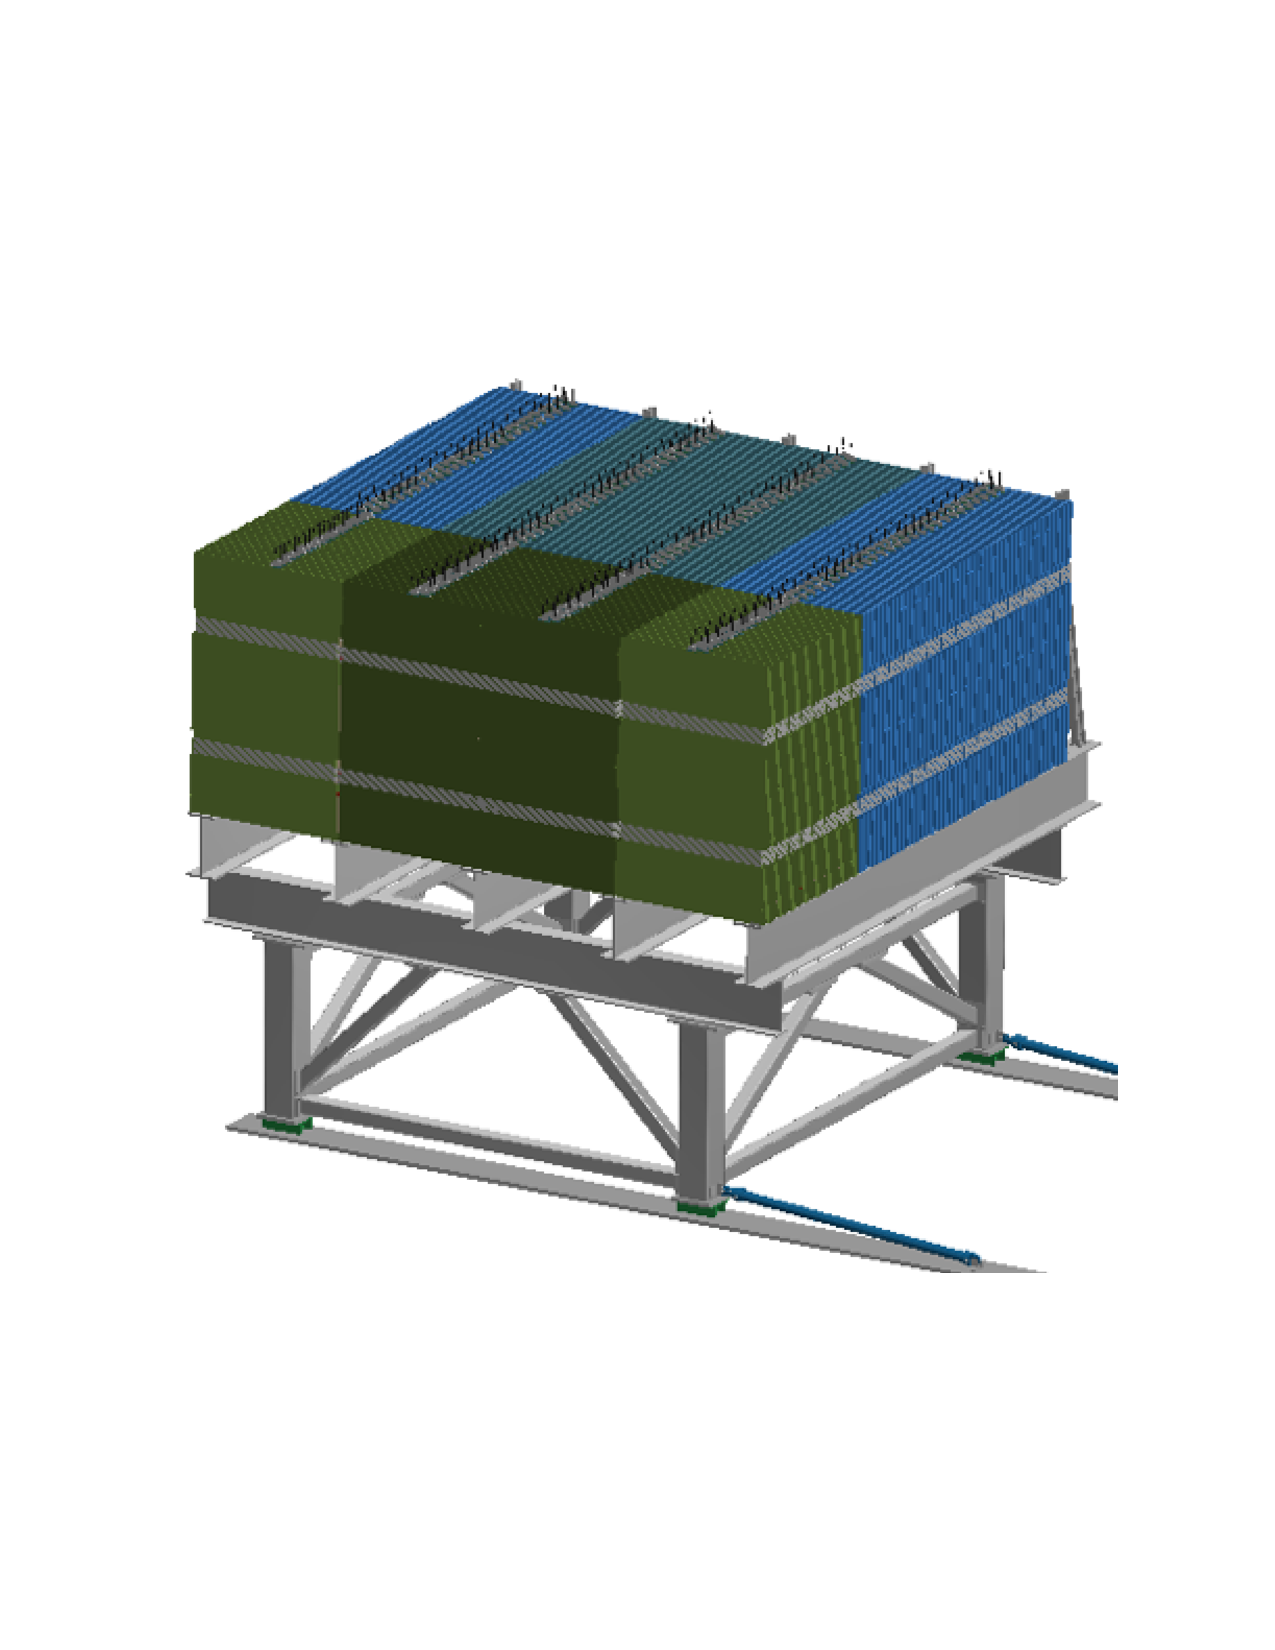
\includegraphics[width=0.8\textwidth]{graphics/Detector/tms_anl_fig1.pdf}
%\end{dunefigure}
%%%%%%%%%%%%%%%
\subsection{Design Parameters}
\label{sec:tms-ovvw-param}

The \dword{dune} \dword{nd} is designed to meet the physics requirements of the \dword{dune} experiment. The eventual statistical uncertainty on the \dword{fd} $\nu_{e}$ rate is less than 3\%, placing stringent requirements on the systematic constraints provided by the \dword{nd}. However, in the early data taking period, the statistical precision of the \dword{fd} will be somewhat worse. As such, the physics goals of the first few years of the \dword{dune} program place less stringent requirements on the \dword{nd}. The \dword{tms} is designed to meet the physics requirements of the initial data taking period of approximately 100 kt-MW-yrs. 

In this period, for $\delta_{CP} = 0$, split equally between horn polarities, 412 (188) oscillated $\nu_{e}$ are expected in \dword{fhc} mode and 84 (176) oscillated $\bar{\nu}_{e}$ in \dword{rhc} mode in the normal (inverted) hierarchy. Thus, the statistical uncertainty on the appearance rate will be $\sim 5-7\%$. Systematic effects at the few percent level, while critical in the long term, do not impact these initial data.

Initial \dword{dune} analyses will use neutrino interactions in the \dword{arcube} detector to predict the \dword{fd} reconstructed event spectra. The reconstruction of the \dword{arcube} events must be as precise as that of the \dword{fd}. Most \dword{fd} muons are identified and their momenta measured by range, with a resolution of 4\% and $4\pi$ angular acceptance. This drives the requirements of the \dword{tms}, which must match this momentum resolution with acceptance that covers the neutrino interaction phase space.
Since the angular acceptance of the \dword{tms} is larger than that of the \dword{ndgar} the acceptance of the \dword{tms} alone is not a limiting factor in the overall performance of the \dword{nd}.
The important design parameters are given in Table~\ref{tab:table-tms-params}, which will apparently be generated from a spreadsheet, though I don't know why or which spreadsheet.

\fixme{Tom: Can you add a few sentences here about sign selection and fringe field requirements.}

\begin{dunetable}
[Placeholder for parameter table]
{cc}
{tab:table-tms-params}
{Placeholder for Parameter Table - it will be generated from a spreadsheet}
Rows & Counts \\ \toprowrule
Row 1 & First \\ \colhline
Row 2 & Second \\ \colhline
Row 3 & Third \\ % no \colhline on final row
\end{dunetable}

%%%%%%%%%%%%%%%Not in Tim's new organization - probably belongs elsewhere
\subsection{Performance}
\subsubsection{Discussion of MINOS performance}
\fixme{Mat will find people to write}
\fixme{Clarence has some of the MINOS docDB documents if needed}

Perhaps the most similar detector to the \dword{tms} is the MINOS
near detector, also comprised of magnetized iron and scintillator. It is, however, not identical: the beam energy is higher, the magnetic field is toroidal, and
the steel is thicker/sampling fraction lower. Nevertheless, it demonstrates what sort of performance might be expected for this choice of technology.

\subsubsection{Software --- Simulation and Analysis}

Neutrino interactions are simulated with \dword{genie} version 2.12.10 using the physics list \texttt{DefaultPlusValenciaMEC}. Particles exiting the struck nucleus are propagated through the \dword{arcube} and \dword{tms} detectors using a Geant4-based model (edep-sim).\fixme{edep-sim needs dword?}
\fixme{citations. github link?}

For most analyses, the signal process is a $\nu_{\mu}$ charged-current interaction in the \dword{arcube} fiducial volume. The outgoing muon exits the \dword{arcube} active volume, passes through the cryostat material, and enters the \dword{tms}. Energy deposits in the active scintillator are recorded and used to reconstruct events.

The analyses presented herein use 10M generated events generated on the \dword{arcube} volume. This results in approximately 4M events with energy deposits in the TMS, and 2M events that are fully contained in the TMS. \fixme{Propose to drop: The files can be found in \texttt{/pnfs/dune/persistent/ndmuonspect}.}

\subsubsection{Geometry Implementation (GDML)}
\fixme{Mat}
A simple Geometry Description Markup Language (GDML) version of the \dword{tms} was created using DUNEggd, an interface to for designing DUNE geometries with the General Geometry Description (GGD) software system. This system was chosen to assure compatibility with existing Near Detector geometries of the ND Hall, \dword{arcube}, GAr, and SAND detectors. 

The geometry consist of 200 layers of alternating steel (7.93 g/cc, 73\% iron, 18\% chromium, 9\% nickel, 0.1\% carbon) and scintillator (1.05 g/cc, 92\% C, 8\% H). The steel is implemented as 3 plates. The central plate is 3.5 m wide by 3.2 m tall. Plates placed to either side of the central plate measure 1.75 m by 3.2 m. A 2 cm gap separates the side plates from the central plate. The first 40 layers of steel are 1.5 cm thick. The rear 60 layers of steel are 4 cm thick. There is a 4 cm gap between each steel layer. 

\fixme{Update these numbers, but we certainly don't have such lareg gaps}
The scintillator is implemented as collection of 3.5~cm wide by 3~m tall by 1~cm thick vertical bars arranged into modules of 1.68 m wide. Four modules are placed side by side with a 70 cm gap between the central modules and 90 cm gaps separating inner and outer modules. These scintillator layers are replicated in the gap between steel layers.  

The steel plates are magnetized in the geometry. The thin (thick) central steel is given a vertically oriented downward pointing field of 1.25 T (0.9 T), while the out steel thin (thick) steel plate have their field pointing upwards with a strength of 1.5 T (1.0 T).

This GDML geometry for the TMS is placed in existing model of the ND Hall with an existing model of the LArTPC. The coordinate system for this geometry is defined with y anti-aligned with gravity, z running horizontally in the direction of the beam, and z align horizontally to the left of the beam direction. The origin is locate at the center point on the hall wall as the beam enters. The TMS is place 8.2 m downstream from the \dword{arcube} (center to center) and 2.51 m below the origin in y.   

Figures \ref{fig:geom_front}-\ref{fig:geom_3d} show the final geometry.

\begin{dunefigure}[]{fig:geom_front}
{Upstream view of the TMS geometry in black and \dword{arcube} in yellow.}
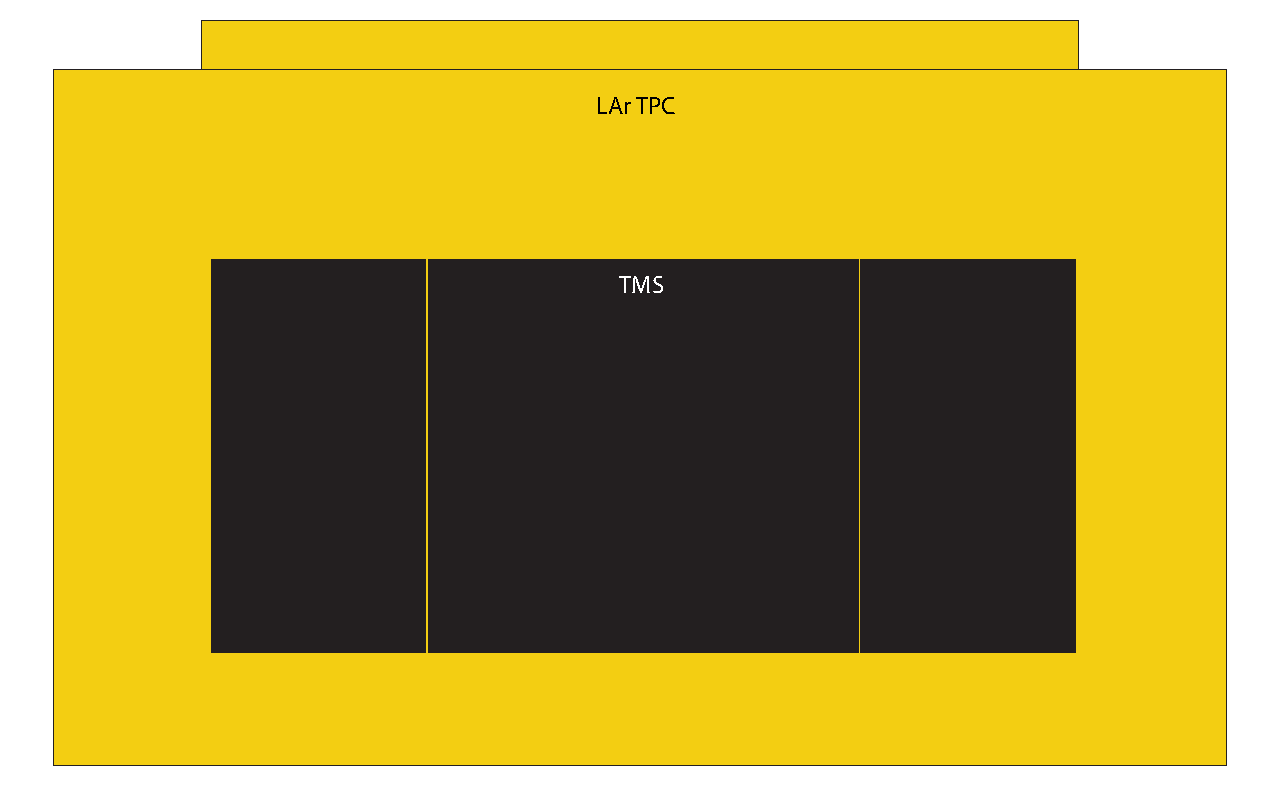
\includegraphics[width=0.8\textwidth]{graphics/Geometry/front_view.pdf}
\end{dunefigure}
\begin{dunefigure}[]{fig:geom_top}
{Top view of the TMS geometry in black and \dword{arcube} in yellow.}
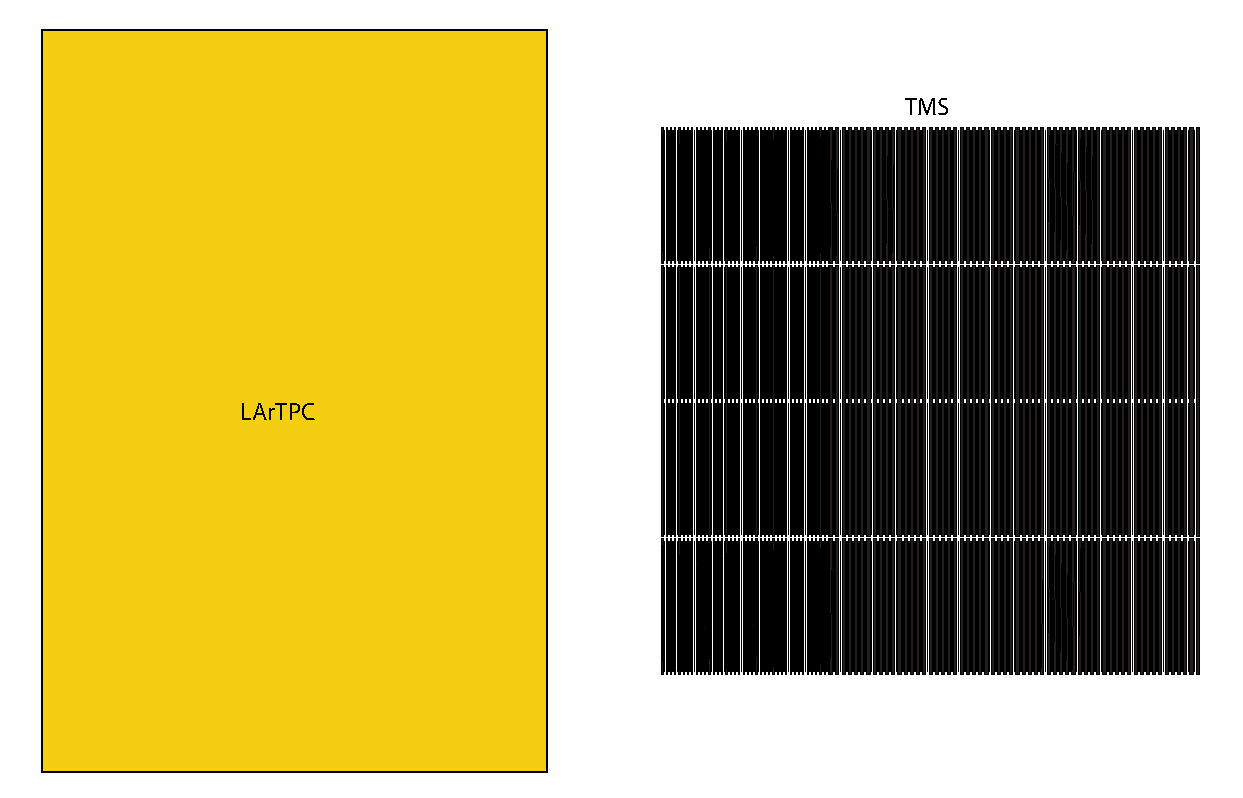
\includegraphics[width=0.8\textwidth]{graphics/Geometry/top_view.pdf}
\end{dunefigure}
\begin{dunefigure}[]{fig:geom_in_hall}
{View of the TMS geometry in grey and \dword{arcube} in orange place in the ND hall. The black line shows the central beam direction. }
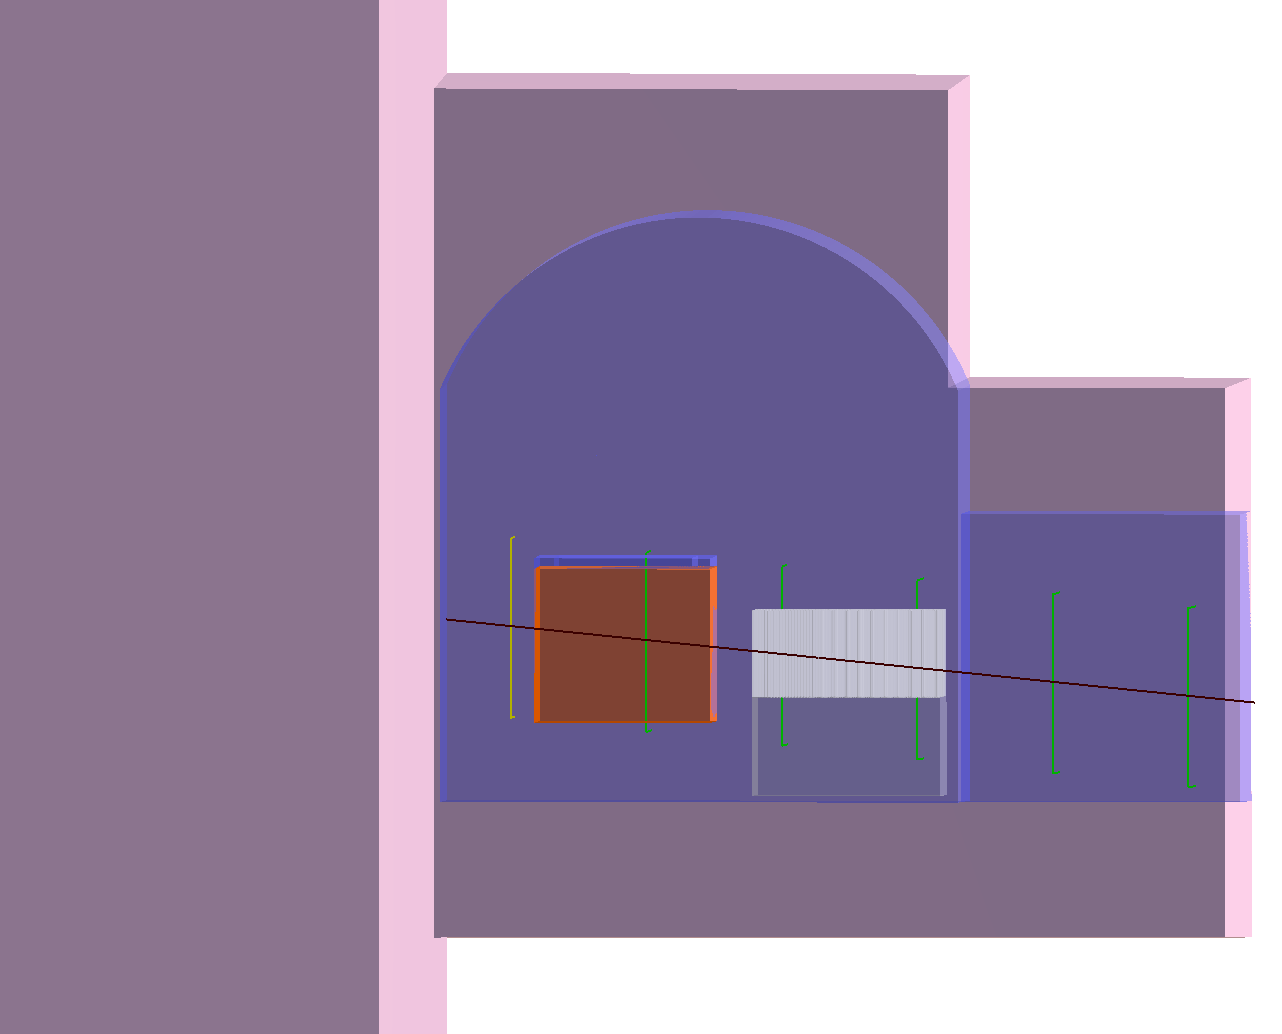
\includegraphics[width=0.8\textwidth]{graphics/Geometry/TMS_LAr.png}
\end{dunefigure}
\begin{dunefigure}[]{fig:geom_3d}
{A perspective view of the TMS geometry in grey and \dword{arcube} in orange.}
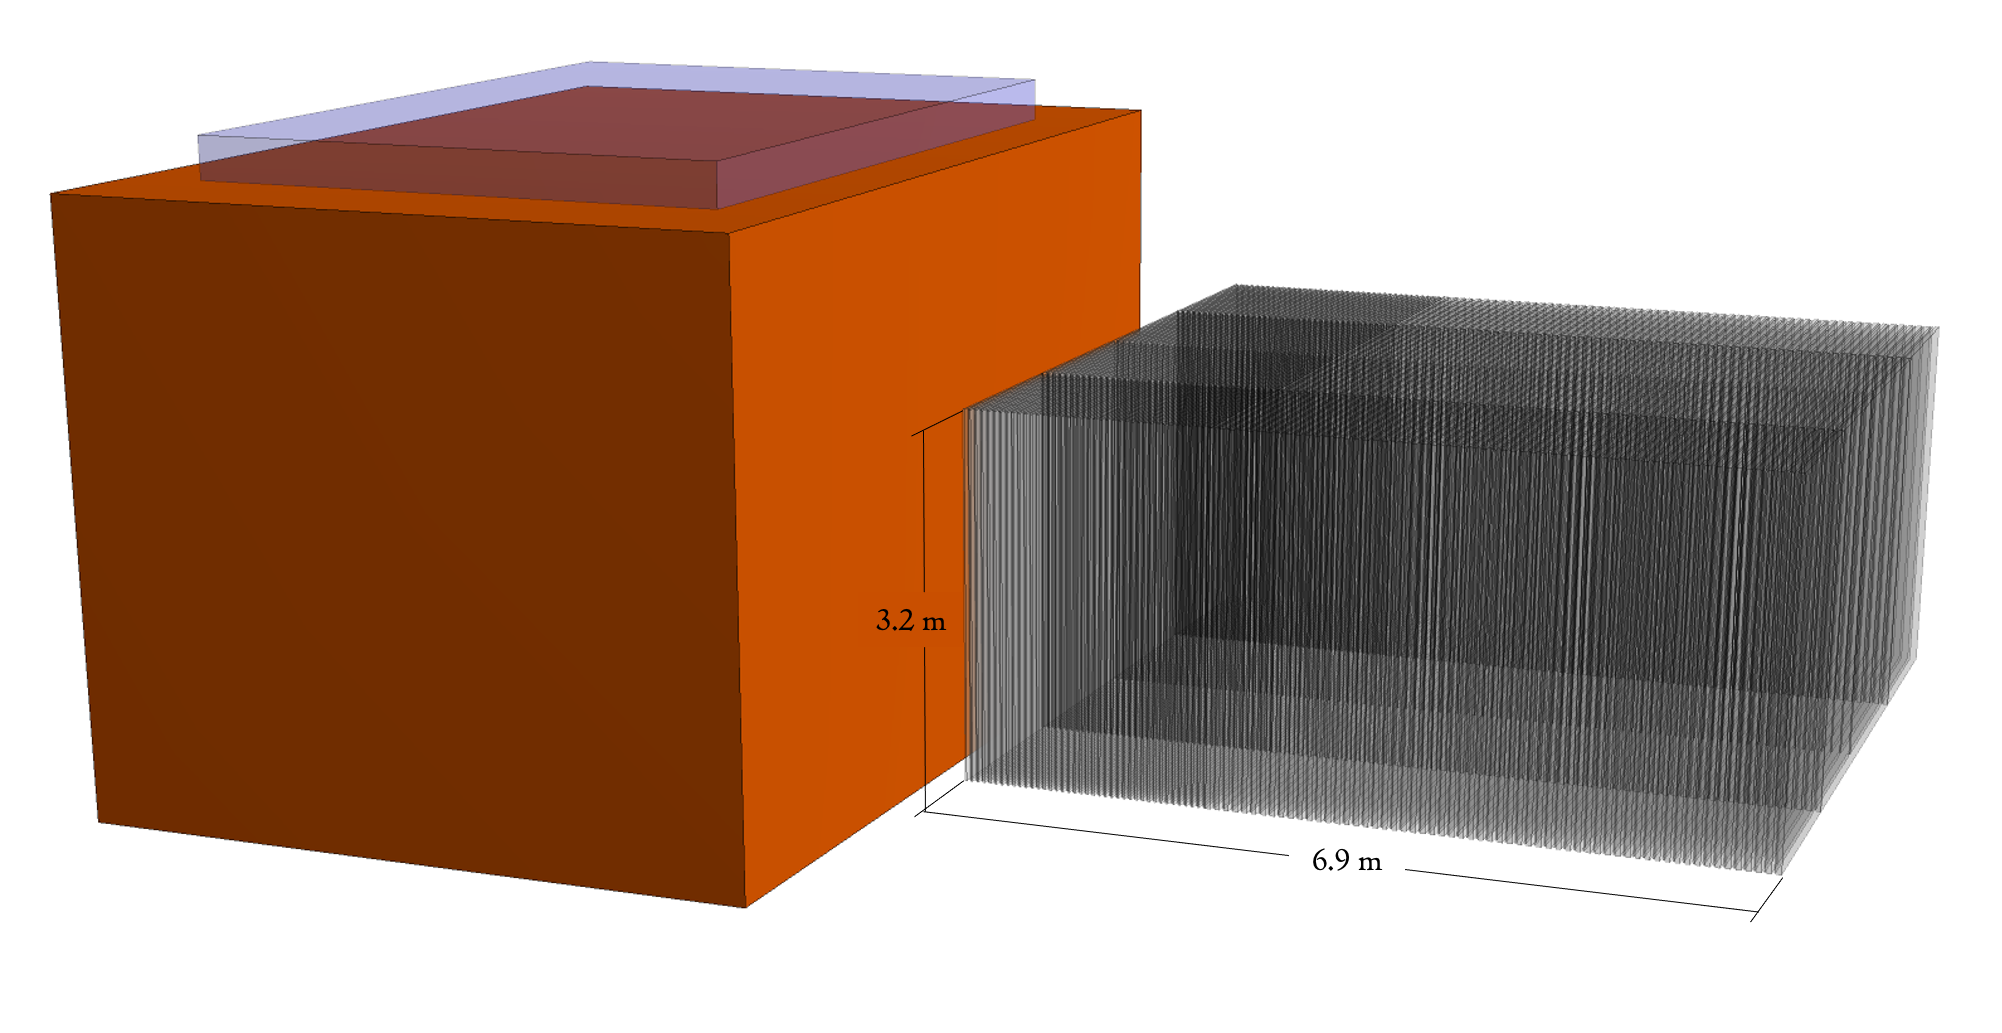
\includegraphics[width=0.8\textwidth]{graphics/Geometry/TMS_LAr_No_Hall.png}
\end{dunefigure}

\subsubsection{Event Gallery}
\fixme{double check dword usage}
% Clarence's notes:
% Show events stopping in the TMS only
% Show opposite bending of neutrino/anti-neutrino events
% Show some different energies and processes
% Show impossible to reconstruct without TMS
This section presents raw event displays, showing the hits from the primary lepton and other particles separated. Both the ArgonCube, gap and \dword{TMS} volumes are shown, as are track start, end and death positions. Each event display is broken down in $x-z$ and $y-z$ views, where the $x-z$ view receives the bending from the magnetic field. We also show the incoming neutrino and outgoing lepton energy and ID, and here only show events that are contained in the TMS. The GENIE event metadata is also included in the title for easy identification of the underlying physics process.

% CCQE event with muon E = 2.84 GeV
\begin{dunefigure}[]{fig:evdisplay_QE}
{A simulated quasi-elastic event with $E_\mu=2.84\text{ GeV}$, split into true lepton hits (top row) and other particle hits (bottom row), with the $x-z$ view on the left, and $y-z$ view on the right. Each display shows ArgonCube (left), the gap region (middle), and the TMS (right). Green boxes represent the detector boundaries, and red dashed boxes the fiducial volumes. The green circle is the lepton production point, the red square in ArgonCube is the exit point, the green square is the TMS entry point, and the red square in the TMS is the stopping point. This event stops just outside the fiducial volume in $y-z$.}
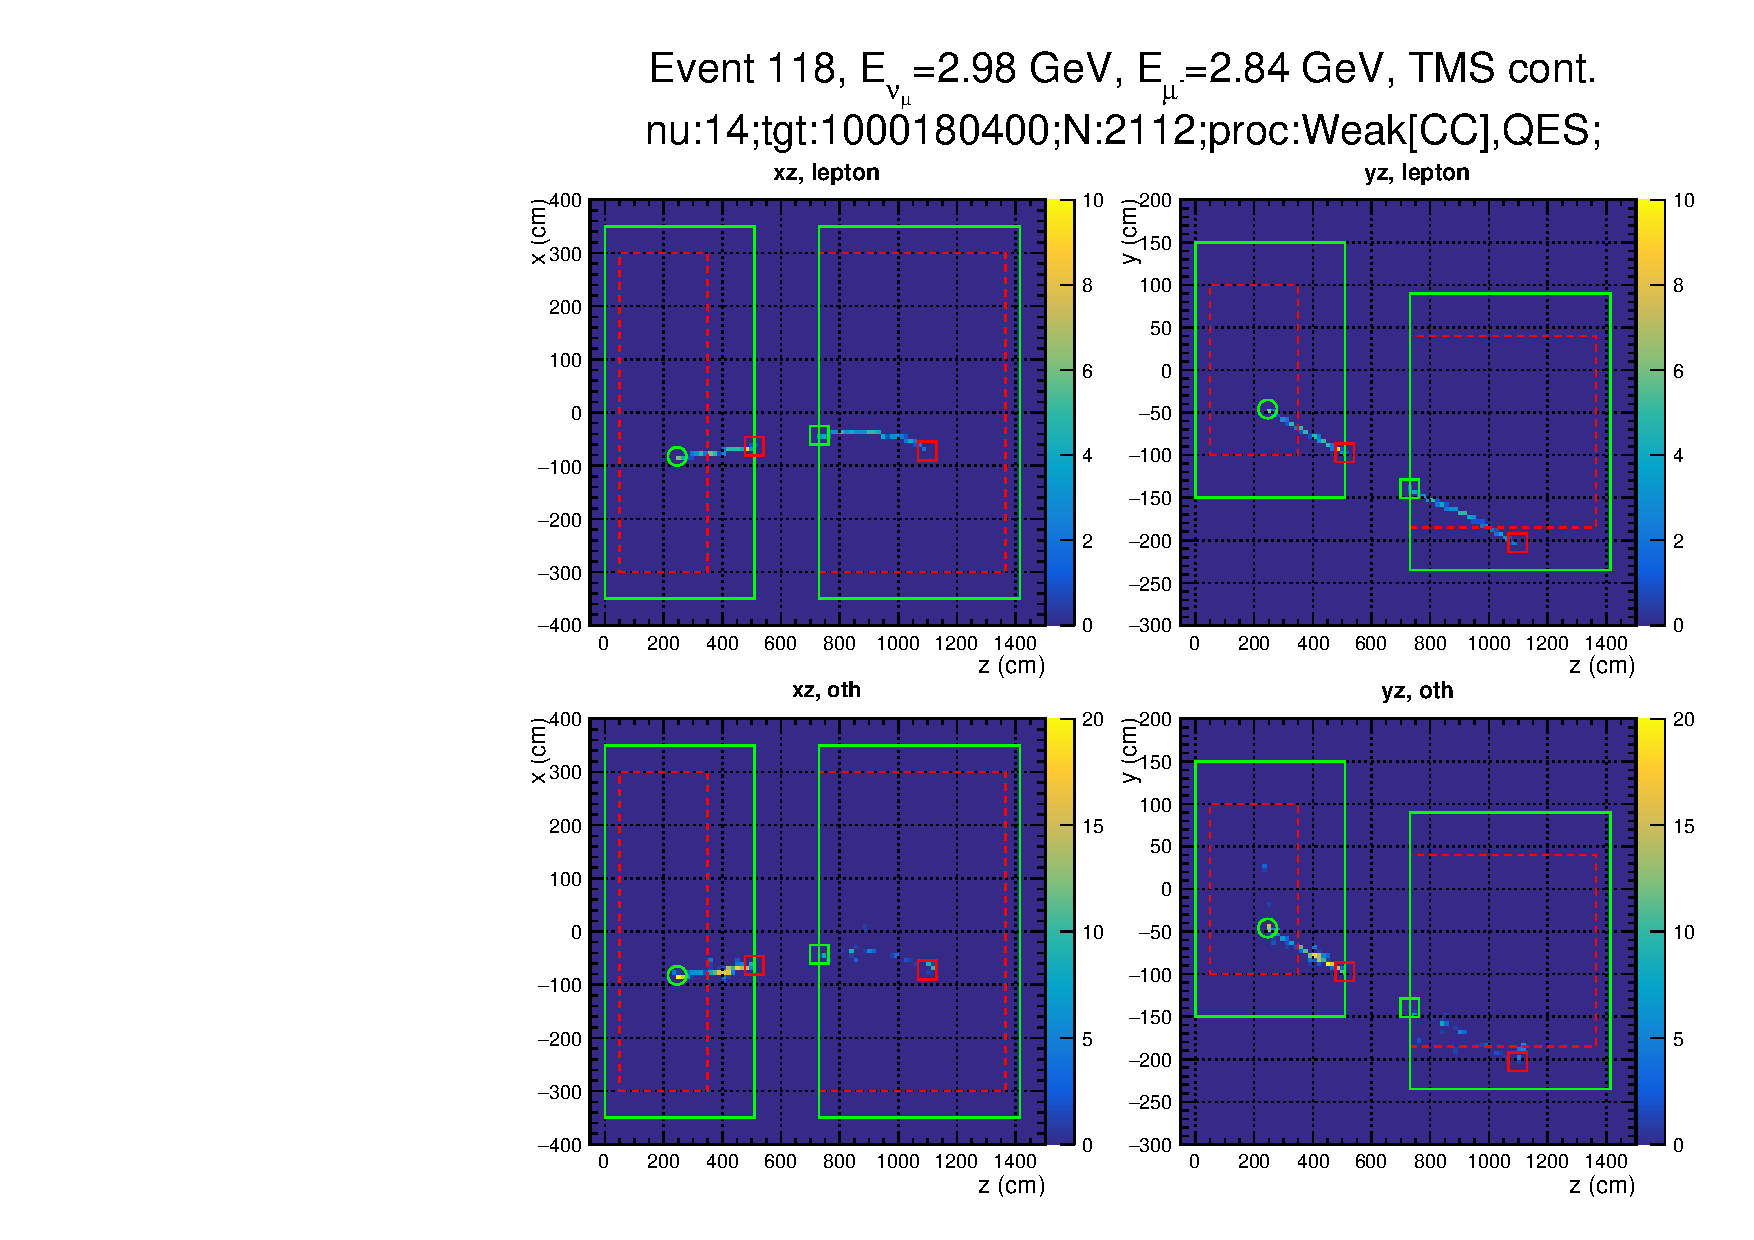
\includegraphics[width=0.8\textwidth]{graphics/Simulation/EventDisplay/pg_0009.pdf}
\end{dunefigure}

% Same CCQE event zoomed in on TMS z
\begin{dunefigure}[]{}
{The event in Figure \ref{fig:evdisplay_QE}, showing true lepton hits in both detectors (top row) and zoomed in on the TMS only (bottom row). The TMS' plane structure in $z$ is visible in the bottom row, where $z<939\text{ cm}$ shows the region with thin iron plates, and $z>949\text{ cm}$ shows the region with thick iron plates.}
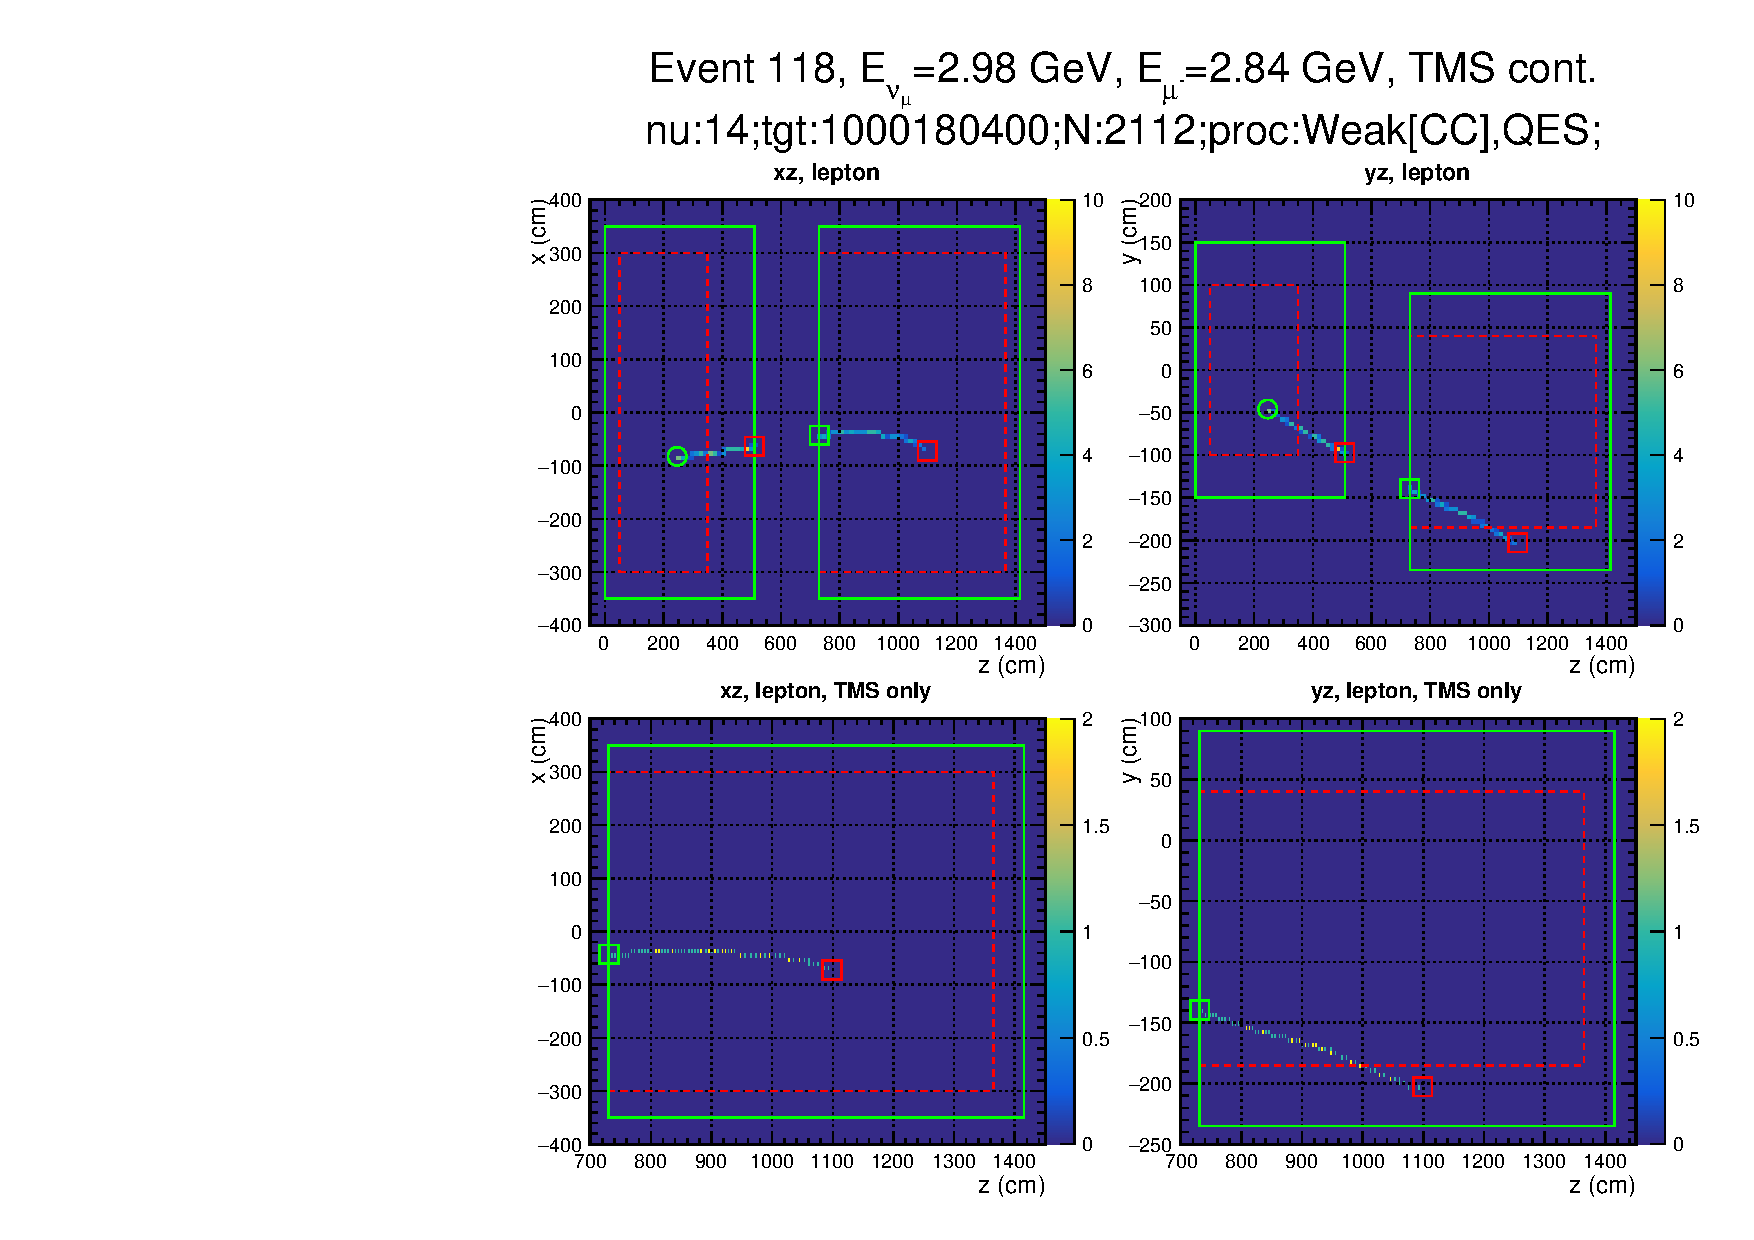
\includegraphics[width=0.8\textwidth]{graphics/Simulation/EventDisplay/pg_0010.pdf}
\end{dunefigure}

% 2p2h anti-neutrino event with similar muon energy, displaying bending
\begin{dunefigure}[optional caption for LoF]{fig:evdisplay_antinu}
{A simulated anti-neutrino 2p2h event with $E_\mu=2.68\text{ GeV}$, split into true lepton hits (top row) and other particle hits (bottom row), with the $x-z$ view on the left, and $y-z$ view on the right. Compared to the CCQE event in Figure \ref{fig:evdisplay_QE} the TMS clearly bends the muon in different directions, enabling sign-selection.}
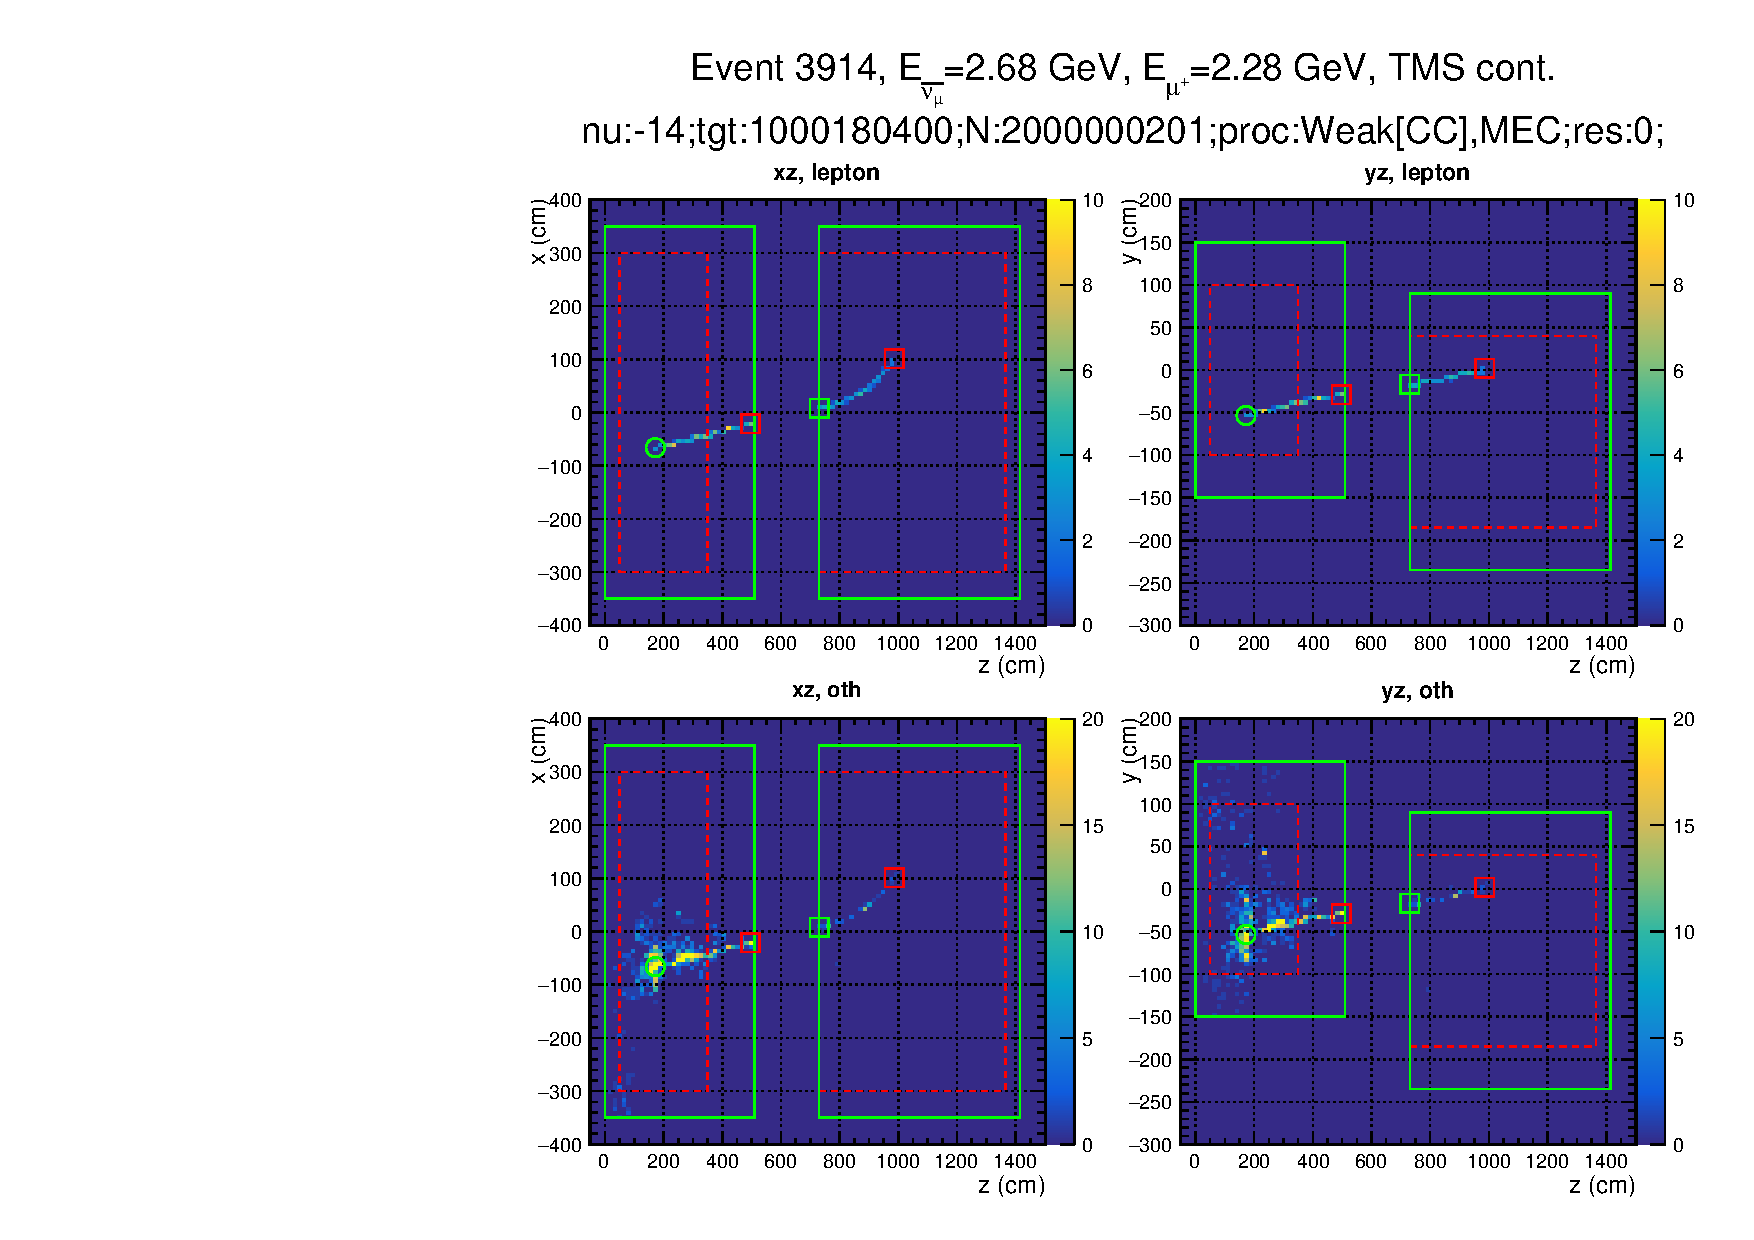
\includegraphics[width=0.8\textwidth]{graphics/Simulation/EventDisplay/pg_0011.pdf}
\end{dunefigure}

% Same 2p2h anti-neutrino event, showing zoomed in on TMS region
\begin{dunefigure}[]{}
{The event in Figure \ref{fig:evdisplay_antinu}, showing true lepton hits in both detectors (top row) and zoomed in on the TMS only (bottom row).}
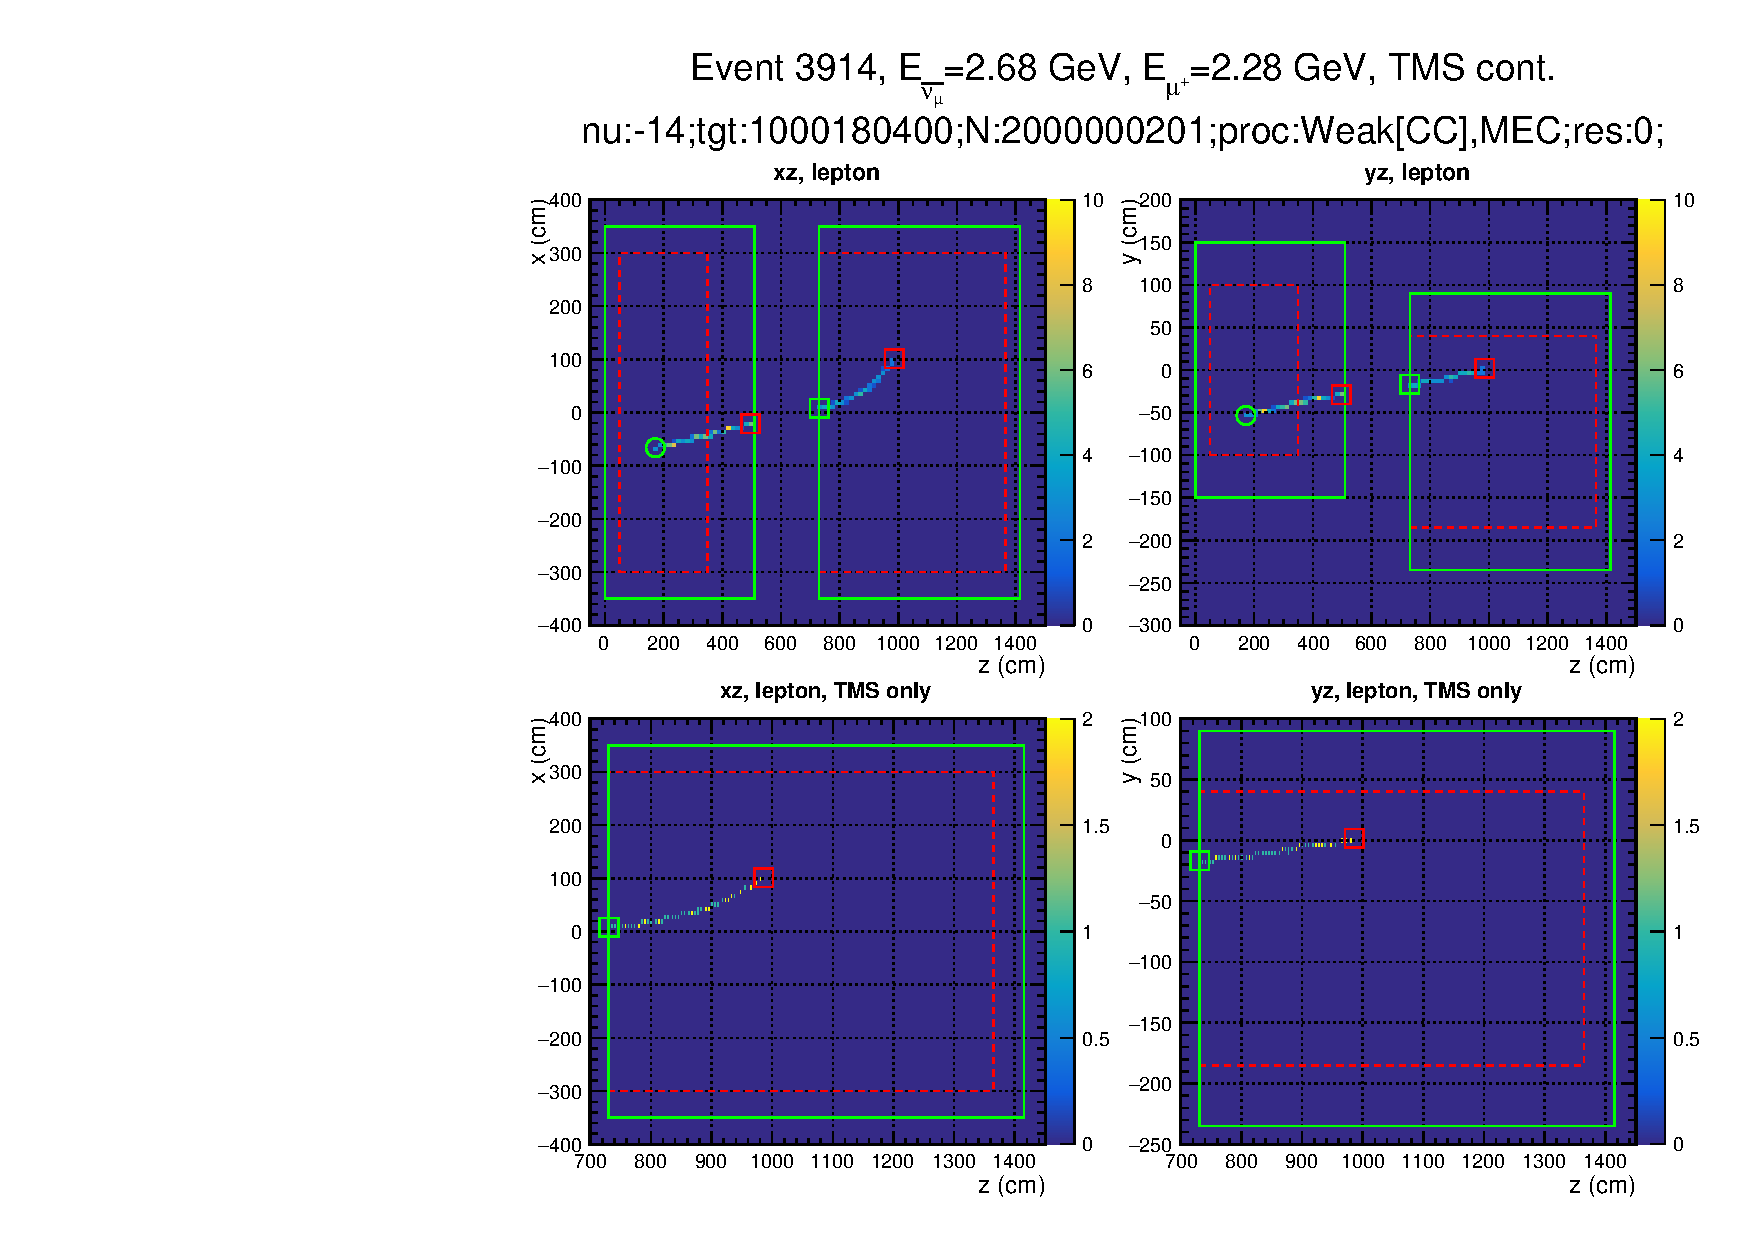
\includegraphics[width=0.8\textwidth]{graphics/Simulation/EventDisplay/pg_0012.pdf}
\end{dunefigure}

% A higher energy event, giving an idea of the top muon energy range for the current design (~5 GeV)
% Also shows that none of the showers in ArgonCube make it to the TMS
\begin{dunefigure}[]{fig:evdisplay_DIS}
{A simulated DIS event with $E_\mu=4.60\text{ GeV}$ and sizeable hadronic energy ($E_{had}\sim2.2\text{ GeV}$), which traverses most of the TMS in $z$. The hadronic showers and sizeable muon kinetic energy in the ArgonCube makes muon identification troublesome without the TMS.}
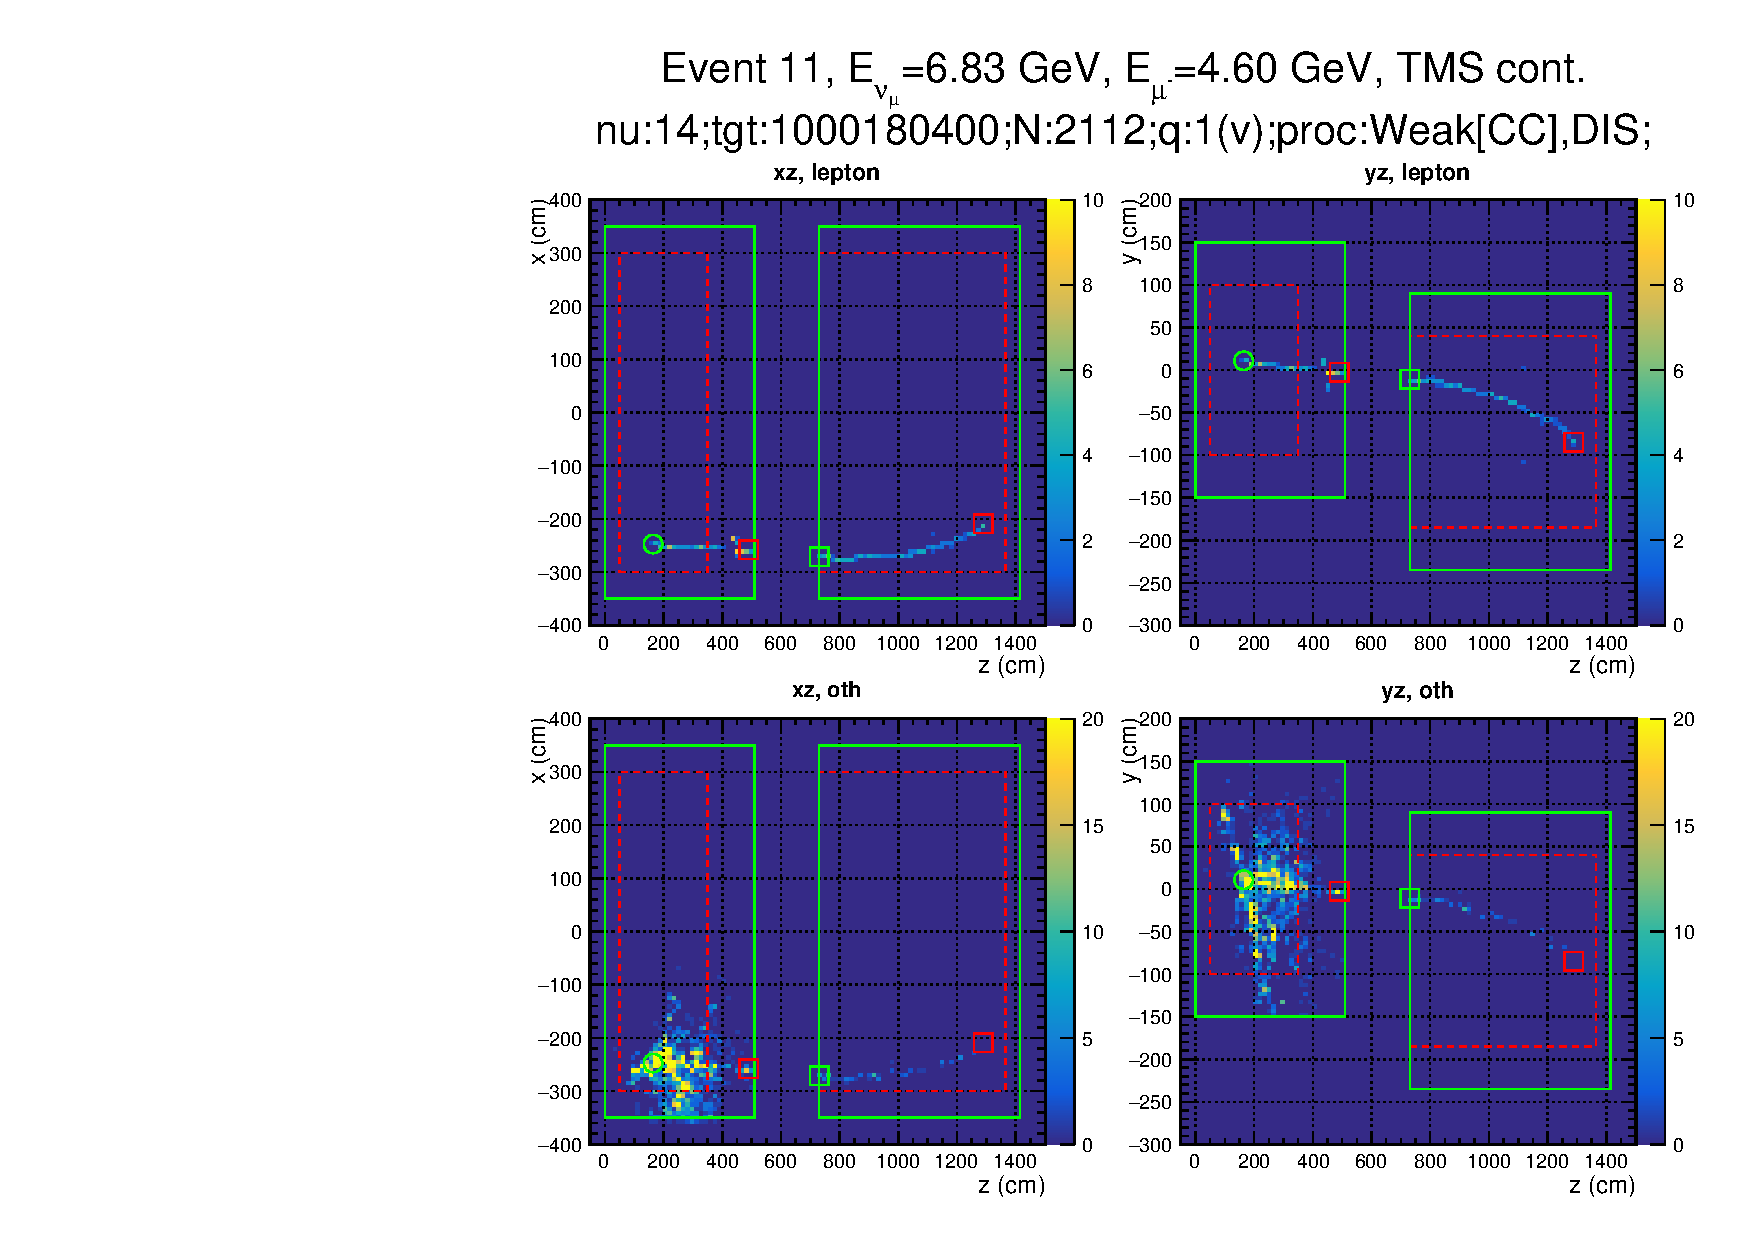
\includegraphics[width=0.8\textwidth]{graphics/Simulation/EventDisplay/pg_0001.pdf}
\end{dunefigure}

% Probably useful to flush pictures out here
\clearpage

\subsubsection{Acceptance}
\fixme{Please use thicker lines if the only distinguishing feature is color; Tom is color-blind}
\fixme{Why do we need TMS stand-alone?}
This section presents preliminary studies using the generated neutrino interactions on the LAr active volume, and calculating the number of events contained in the LAr and TMS detectors compared to the total. We use the true generated positions to calculate all efficiencies as a full reconstruction is not yet available.

The TMS is directly downstream of the LAr, so greatly improves the forward-going acceptance of the combined LAr+TMS system. Figure \ref{fig:eff_th} shows the acceptance in $\theta_{\nu,\mu}$ using the average neutrino direction. We see the TMS does well to compensate for the LAr acceptance at low $\theta_{\nu,\mu}$, and has a maximum efficiency of $\sim45\%$ at $\theta_{\nu,\mu}\sim10\degree$. The lowest efficiency for the combined LAr+TMS system is at $\theta_{\nu,\mu}\sim 30\degree$, at which it is 30\%.
% acceptance in muon/neutrino angle
\begin{dunefigure}[]{fig:eff_th}
{Efficiency of the LAr, TMS and combined system in $\theta_{\nu,\mu}$. Left shows the events contained in the different detectors, compared with all events. Right shows the ratio of each category relative the total.}
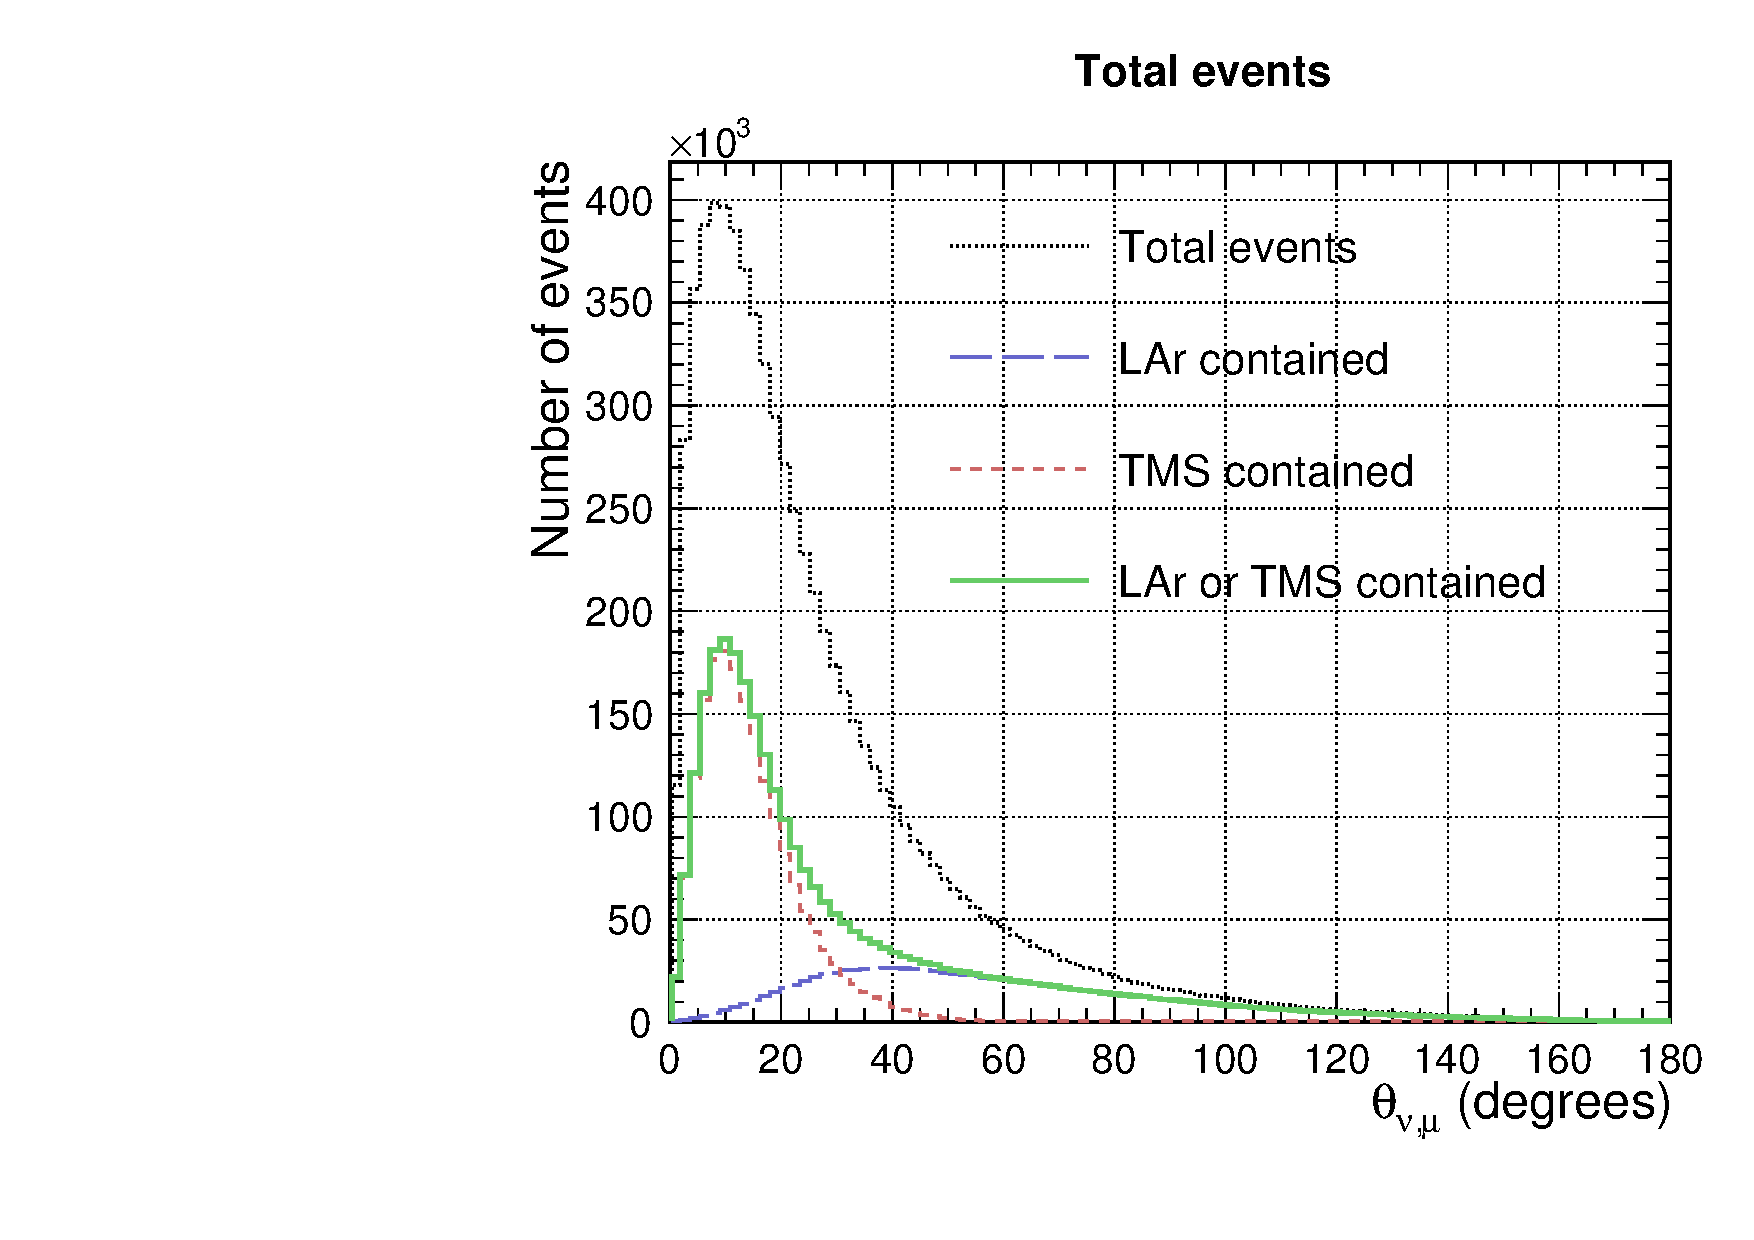
\includegraphics[width=0.49\textwidth, clip, trim={0mm 0mm 0mm 10mm}]{graphics/Simulation/Efficiency/eff_theta.pdf} 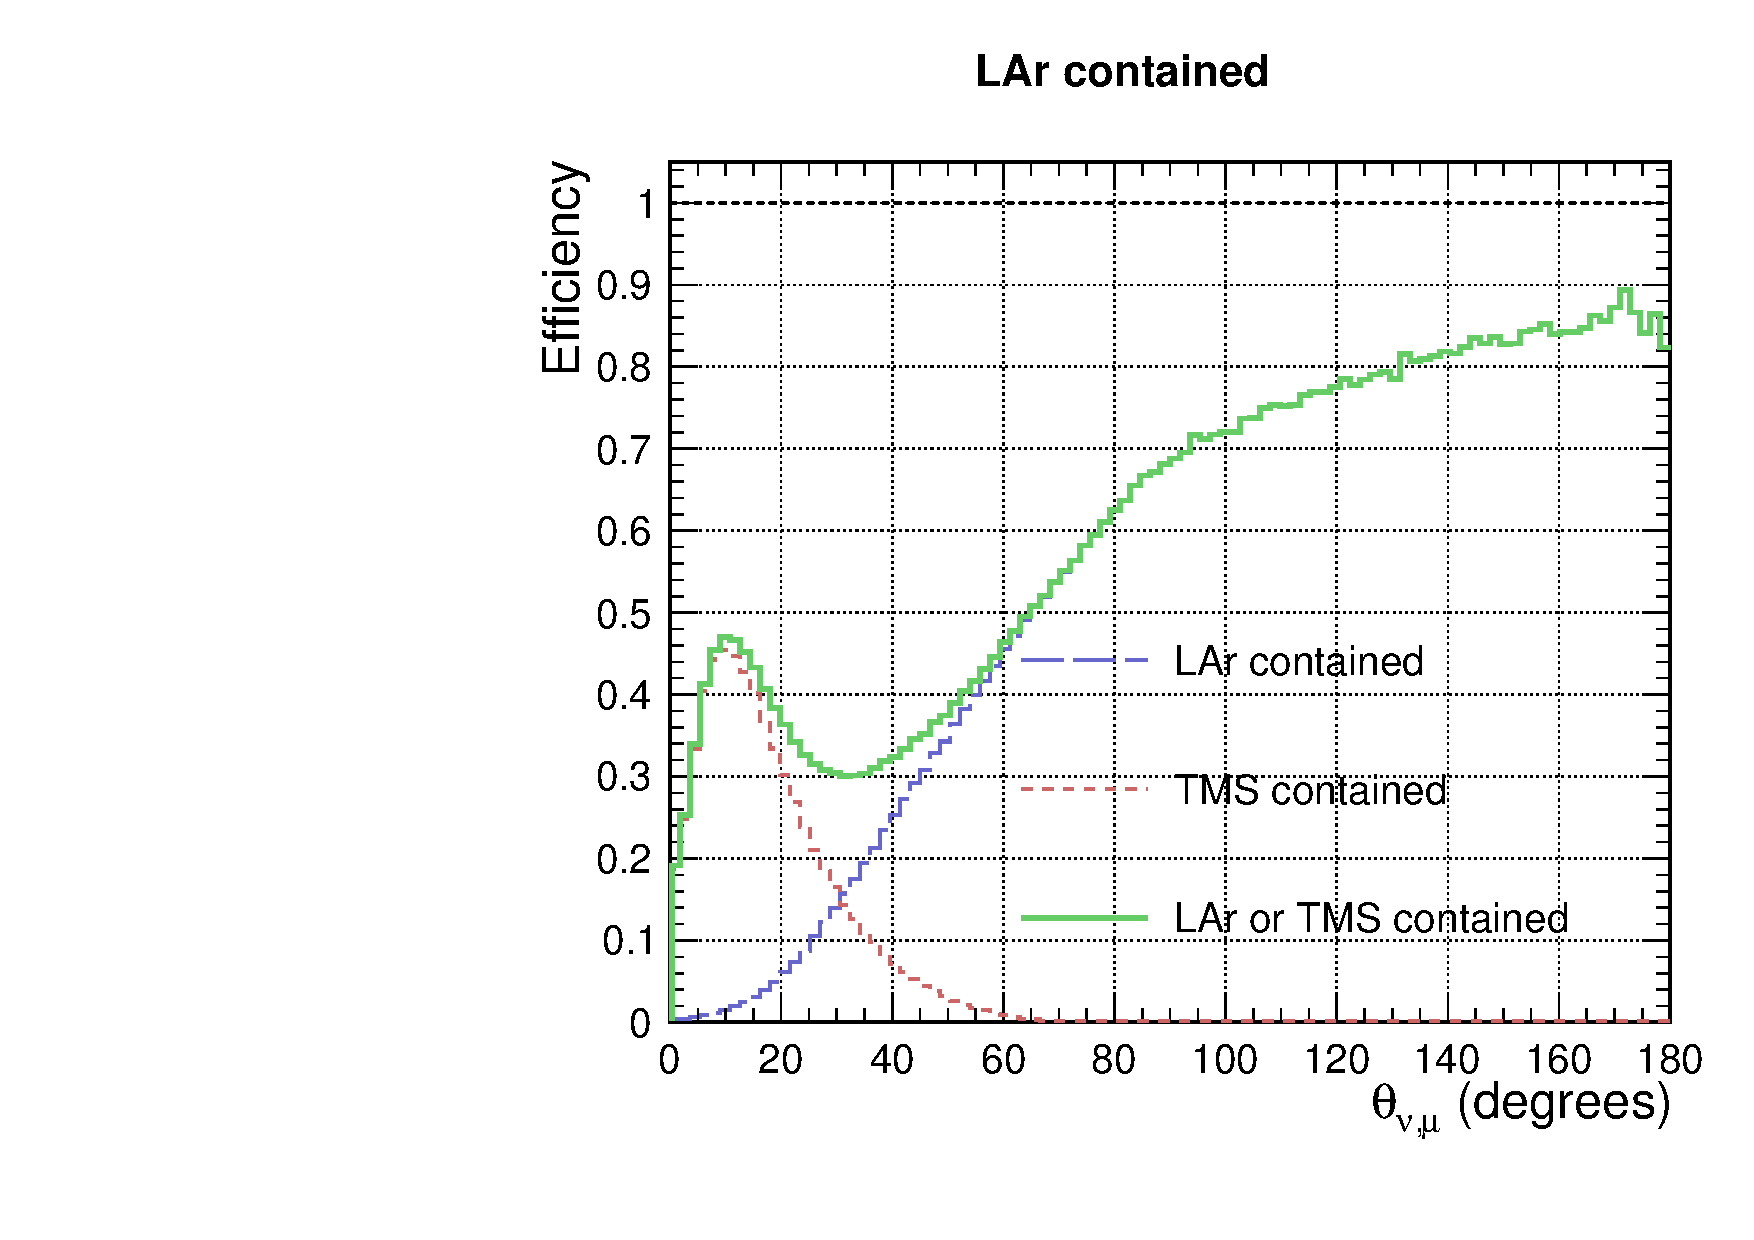
\includegraphics[width=0.49\textwidth, clip, trim={0mm 0mm 0mm 10mm}]{graphics/Simulation/Efficiency/eff_theta_ratio.pdf}
\end{dunefigure}

Figure \ref{fig:eff_enu} shows the efficiency as a function of incoming neutrino energy ($E_\nu$) in FHC for the unrestricted phase space. We see the LAr performing well at low neutrino energy, with $>40\%$ efficiency when $E_\nu < 1 \text{ GeV}$. It rapidly falls with increasing neutrino energy, and is $\sim15\%$ at the $E_\nu\sim 2.5\text{ GeV}$ peak. The TMS acceptance rises steadily as the LAr acceptance drops, leading to a combined flat acceptance of $\sim45\%$ between $2.0<E_\nu<4.0\text{ GeV}$.
% Overall acceptance in neutrino energy
\begin{dunefigure}[]{fig:eff_enu}
{Efficiency of the LAr, TMS and combined system in $E_\nu^\text{True}$. Left shows the events contained in the different detectors, compared with all events. Right shows the ratio of each category relative the total.}
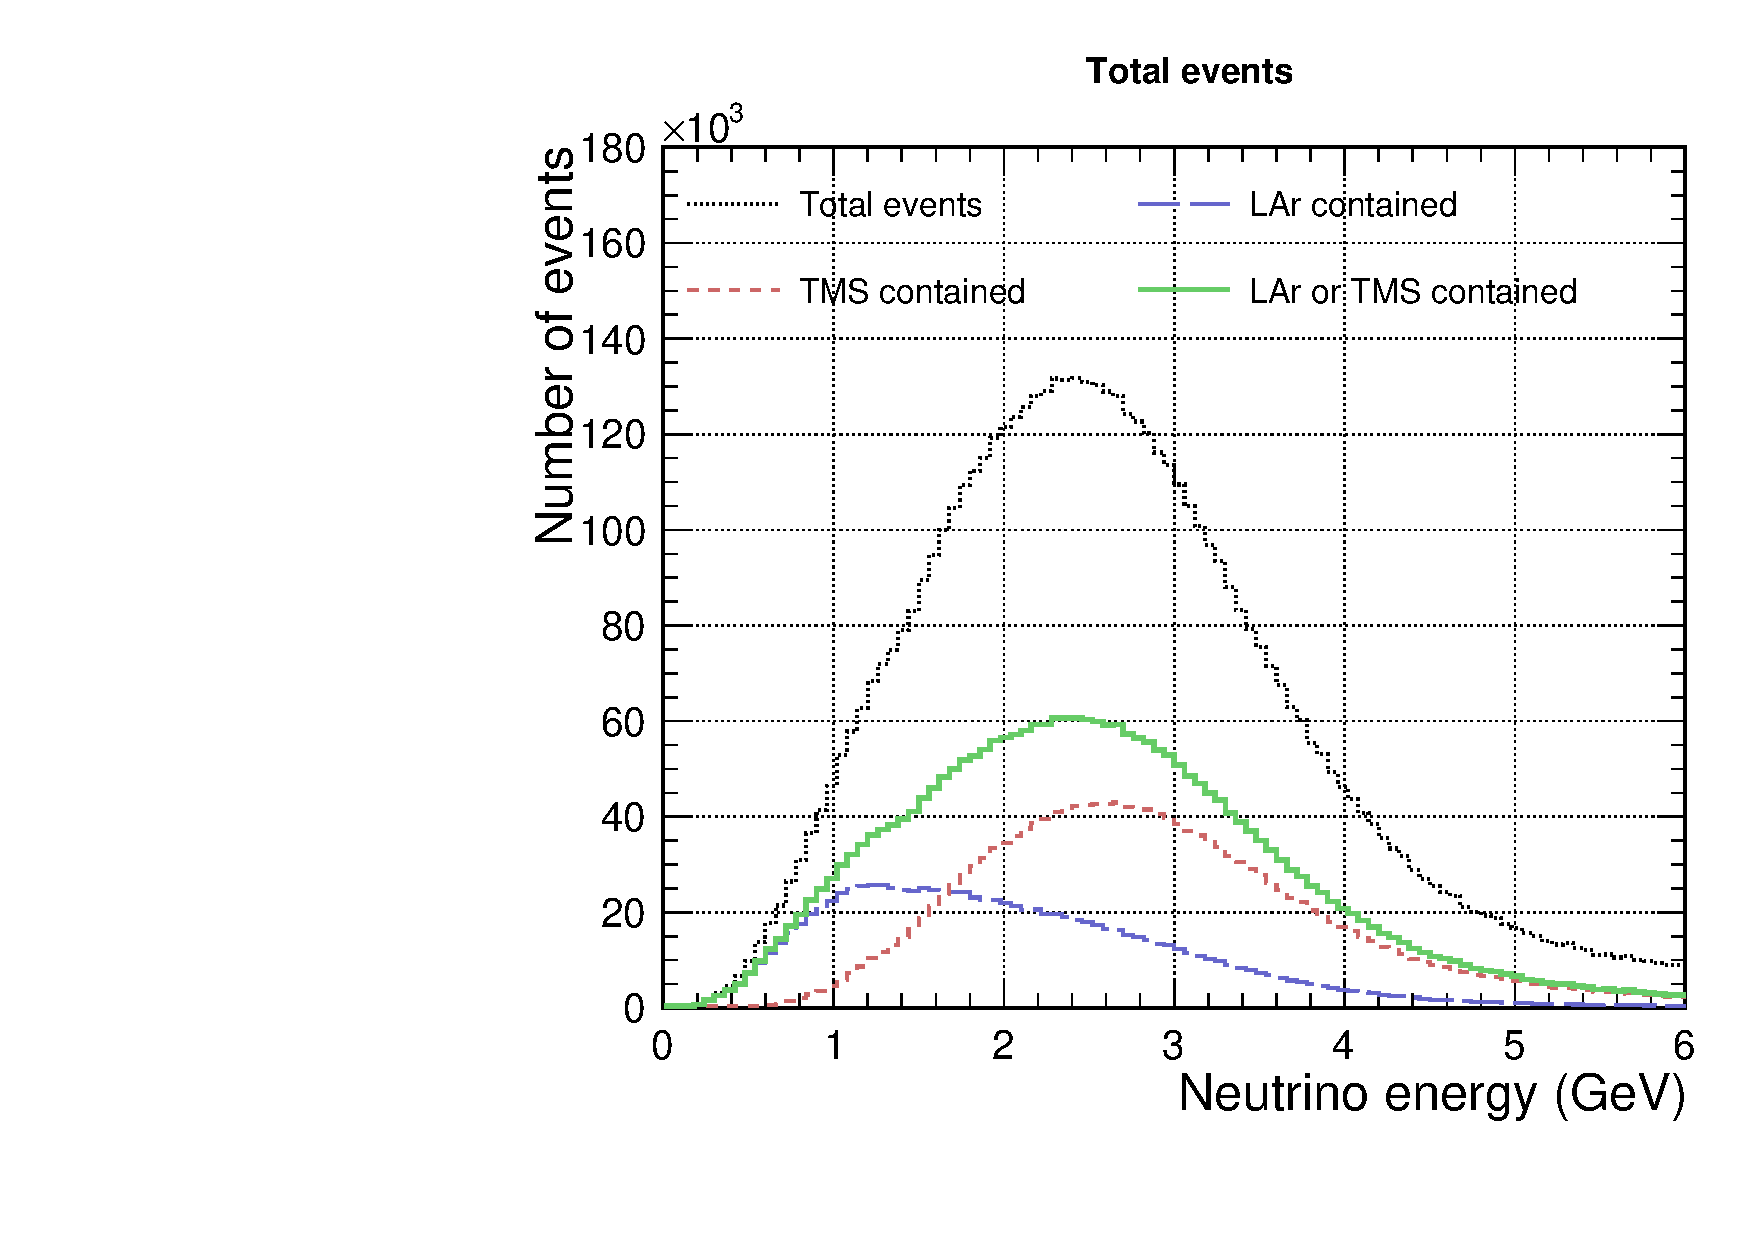
\includegraphics[width=0.49\textwidth, clip, trim={0mm 0mm 0mm 10mm}]{graphics/Simulation/Efficiency/eff.pdf} 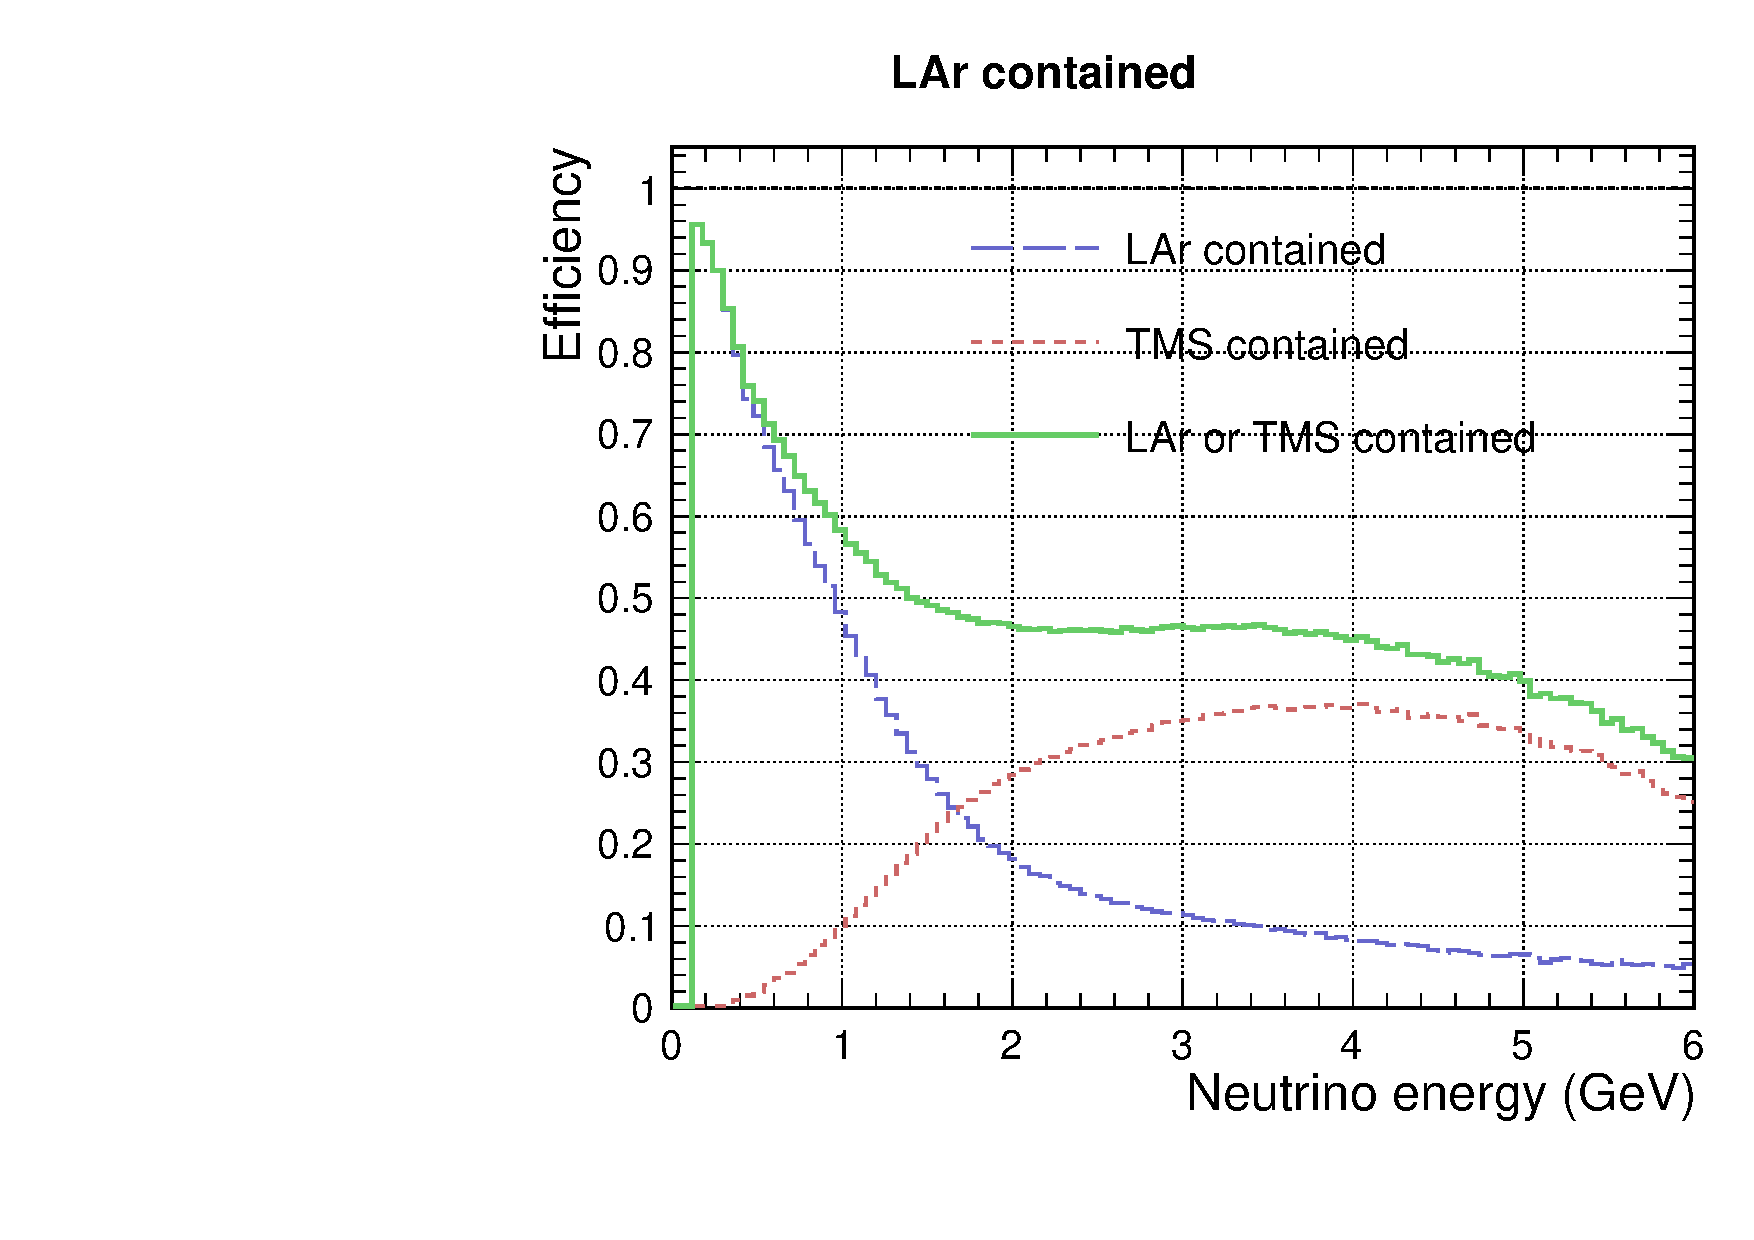
\includegraphics[width=0.49\textwidth, clip, trim={0mm 0mm 0mm 10mm}]{graphics/Simulation/Efficiency/eff_ratio.pdf}
\end{dunefigure}

In Figure \ref{fig:eff_enu_th20} we repeat the acceptance study in $E_\nu$, but include a $\theta_{\nu,\mu}<20\degree$ cut to better characterise the LAr+TMS acceptance. We see the LAr efficiency drop more aggressively with increasing neutrino energy with the $\theta_{\nu,\mu}$ cut, reaching 10\% at $E_\nu\sim 1.5\text{ GeV}$. However, the TMS efficiency rises at a similar rate, peaking at $E_\nu\sim1.9\text{ GeV}$ with 55\% acceptance. The overall acceptance drops below 50\% when $E_\nu>4.5\text{ GeV}$.
% Overall acceptance in neutrino energy
\begin{dunefigure}[]{fig:eff_enu_th20}
{Efficiency of the LAr, TMS and combined system in $E_\nu^\text{True}$ with $\theta_{\nu,\mu}<20\degree$. Left shows the events contained in the different detectors, compared with all events. Right shows the ratio of each category relative the total.}
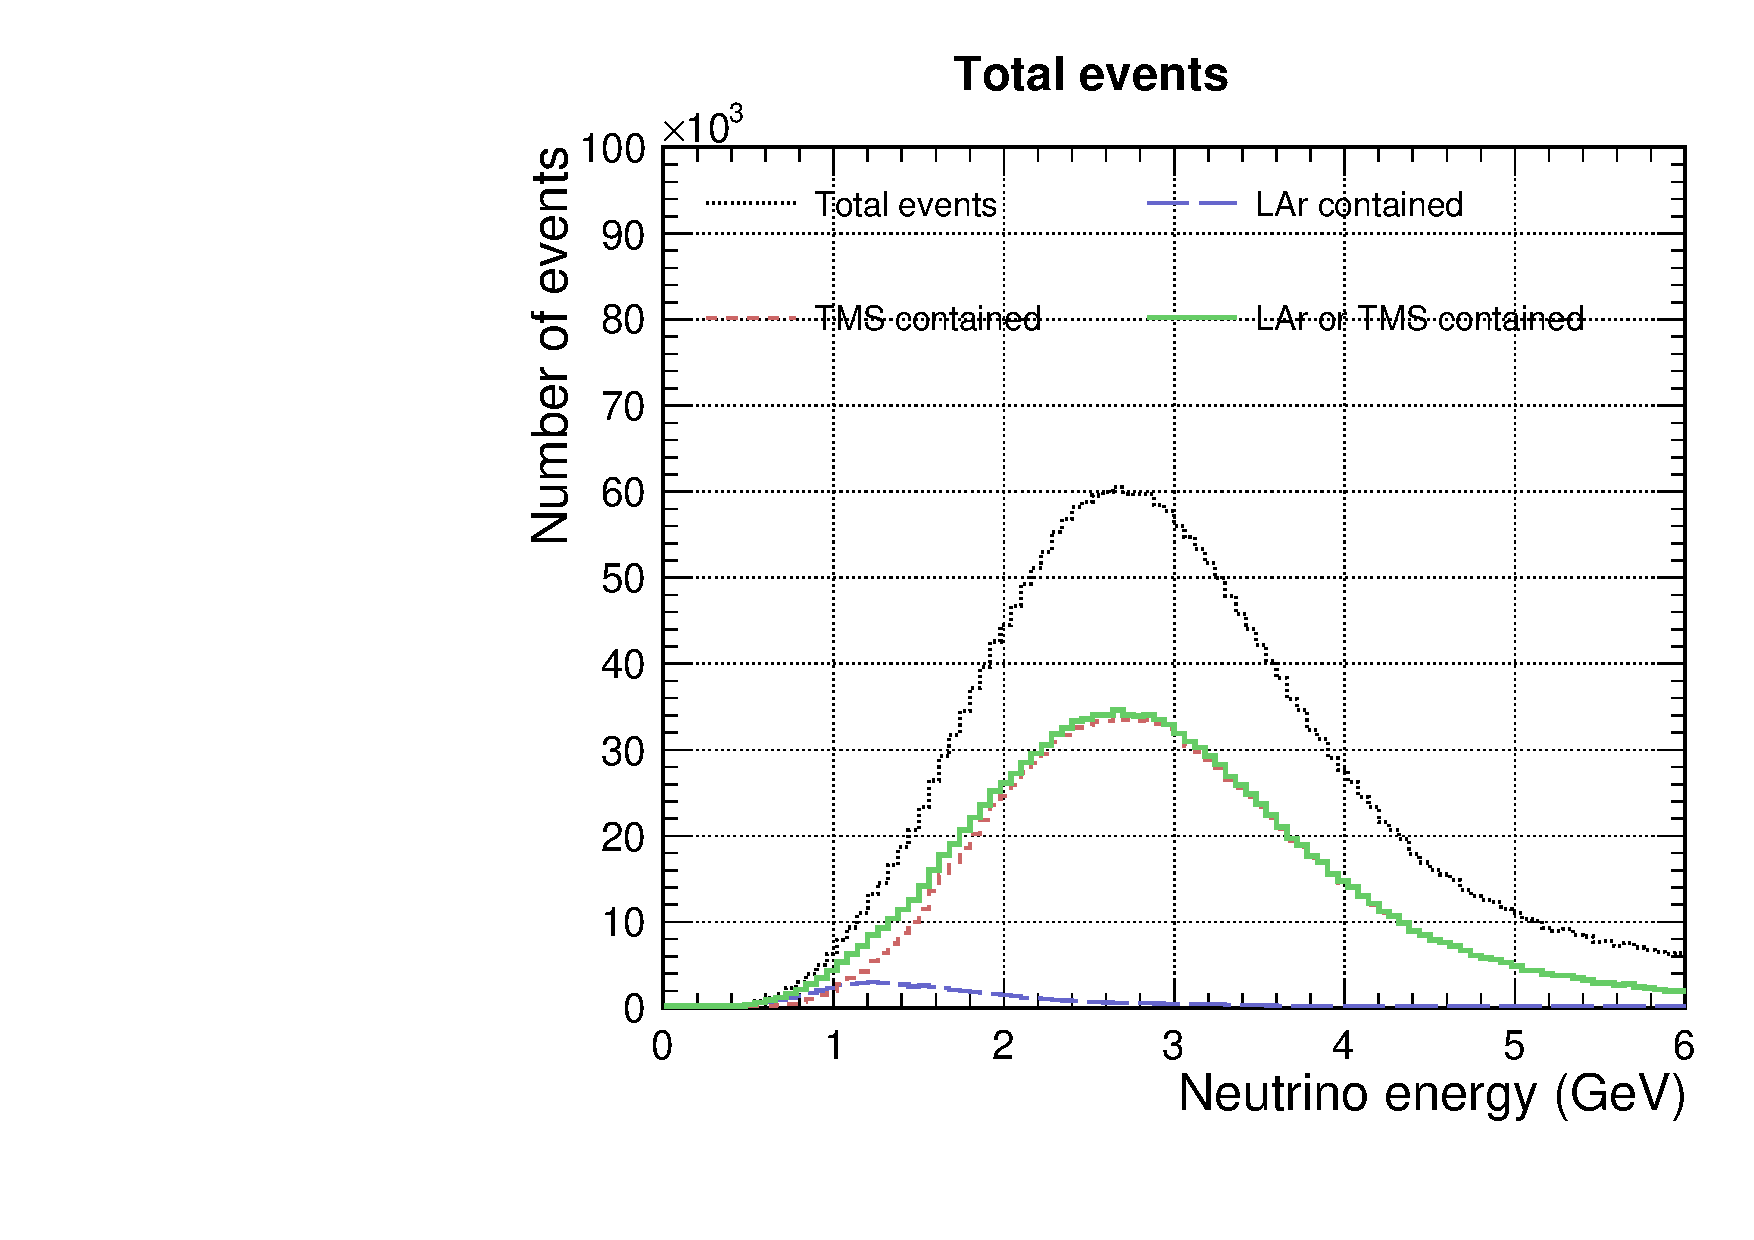
\includegraphics[width=0.49\textwidth, clip, trim={0mm 0mm 0mm 10mm}]{graphics/Simulation/Efficiency/eff_20deg.pdf} 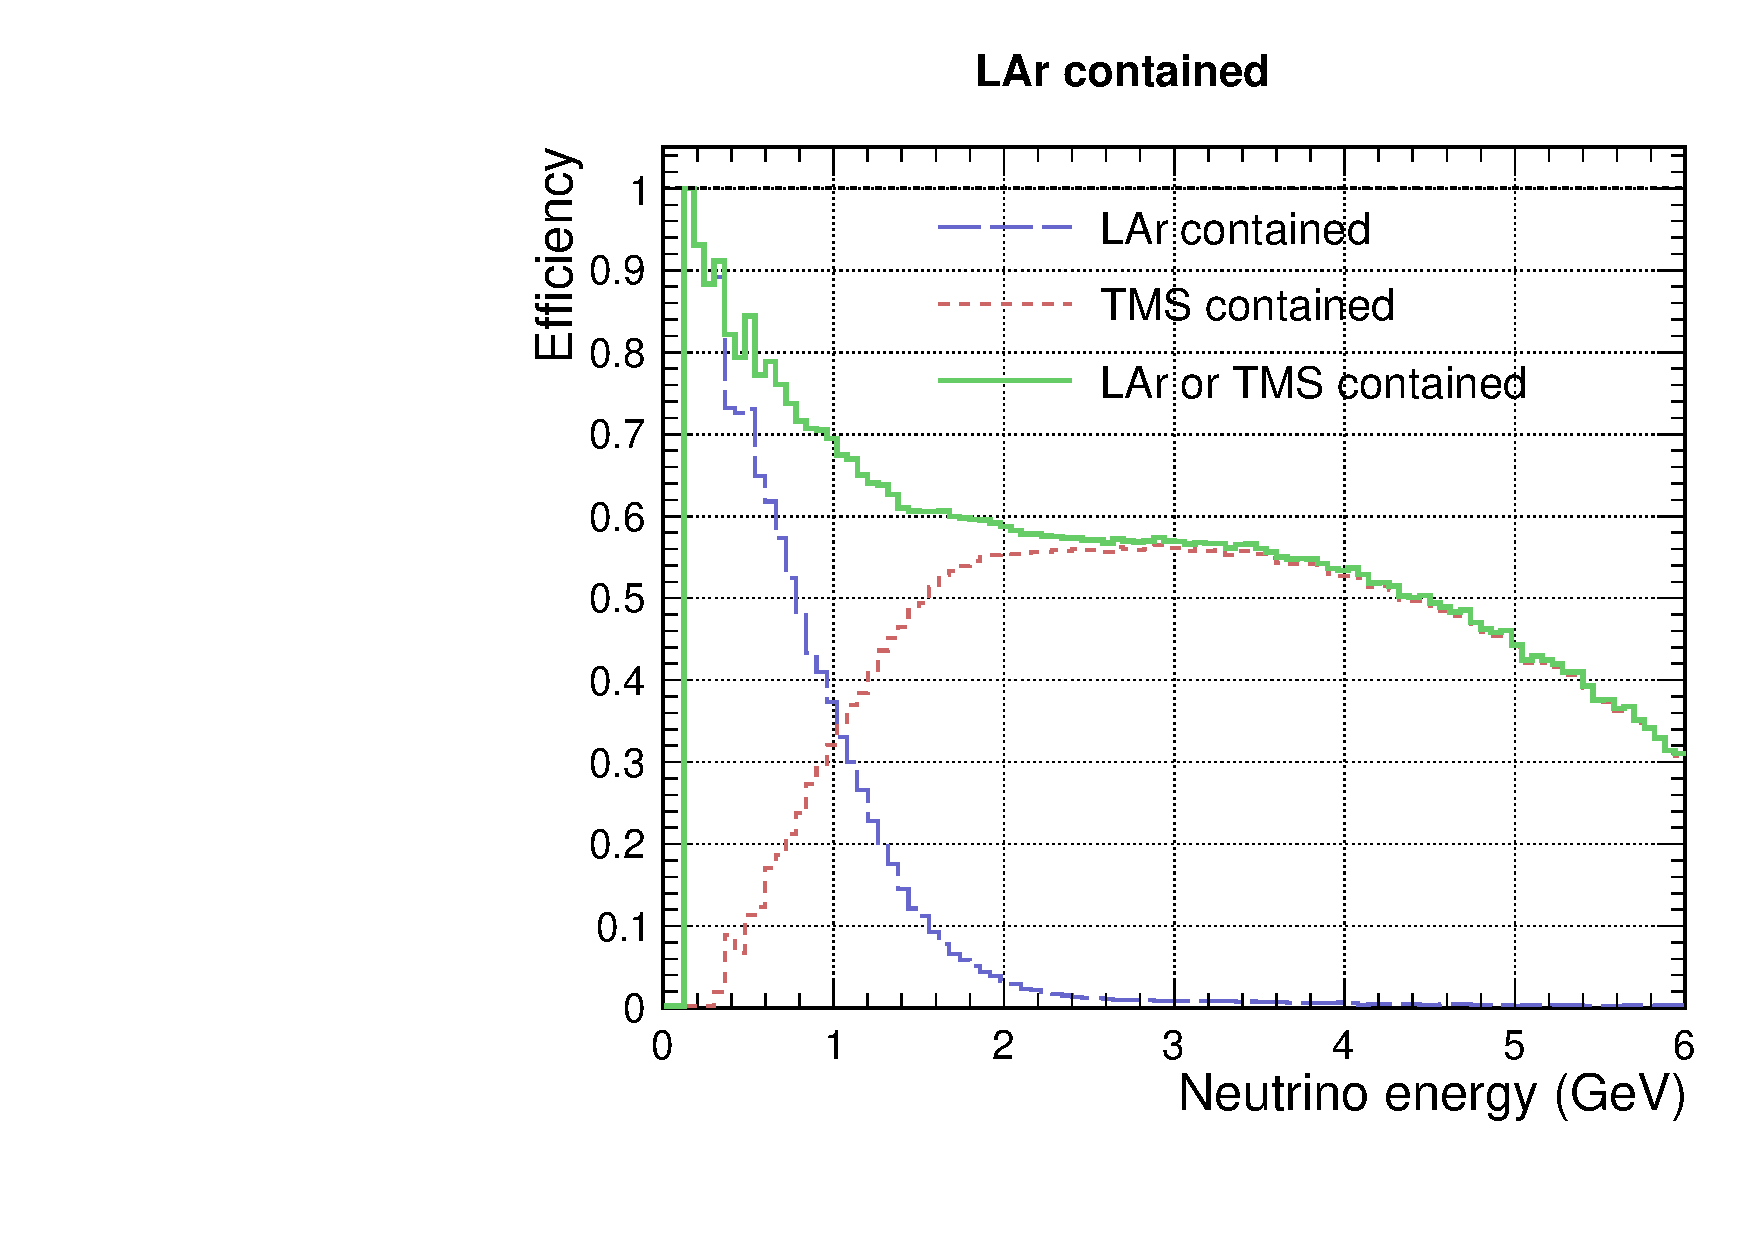
\includegraphics[width=0.49\textwidth, clip, trim={0mm 0mm 0mm 10mm}]{graphics/Simulation/Efficiency/eff_ratio_20deg.pdf}
\end{dunefigure}

Finally, Figure \ref{fig:eff_ke} shows the acceptance in muon kinetic energy after the neutrino interaction in the LAr without any angular cuts. The LAr contained events drop rapidly as the total events reaches its peak at 500 MeV. The TMS acceptance is low at low kinetic energies, mostly due to the muons not making it into the TMS and this acceptance including all $\theta_{\nu,\mu}$. The LAr+TMS acceptance is dominated by the TMS above $T_\mu=1\text{ GeV}$, and rises to 50\% at 3 GeV. 
% Overall acceptance in LAr KE
\begin{dunefigure}[]{fig:eff_ke}
{Efficiency of the LAr, TMS and combined system in $T_\mu$ in the LAr. Left shows the events contained in the different detectors, compared with all events. Right shows the ratio of each category relative the total.}
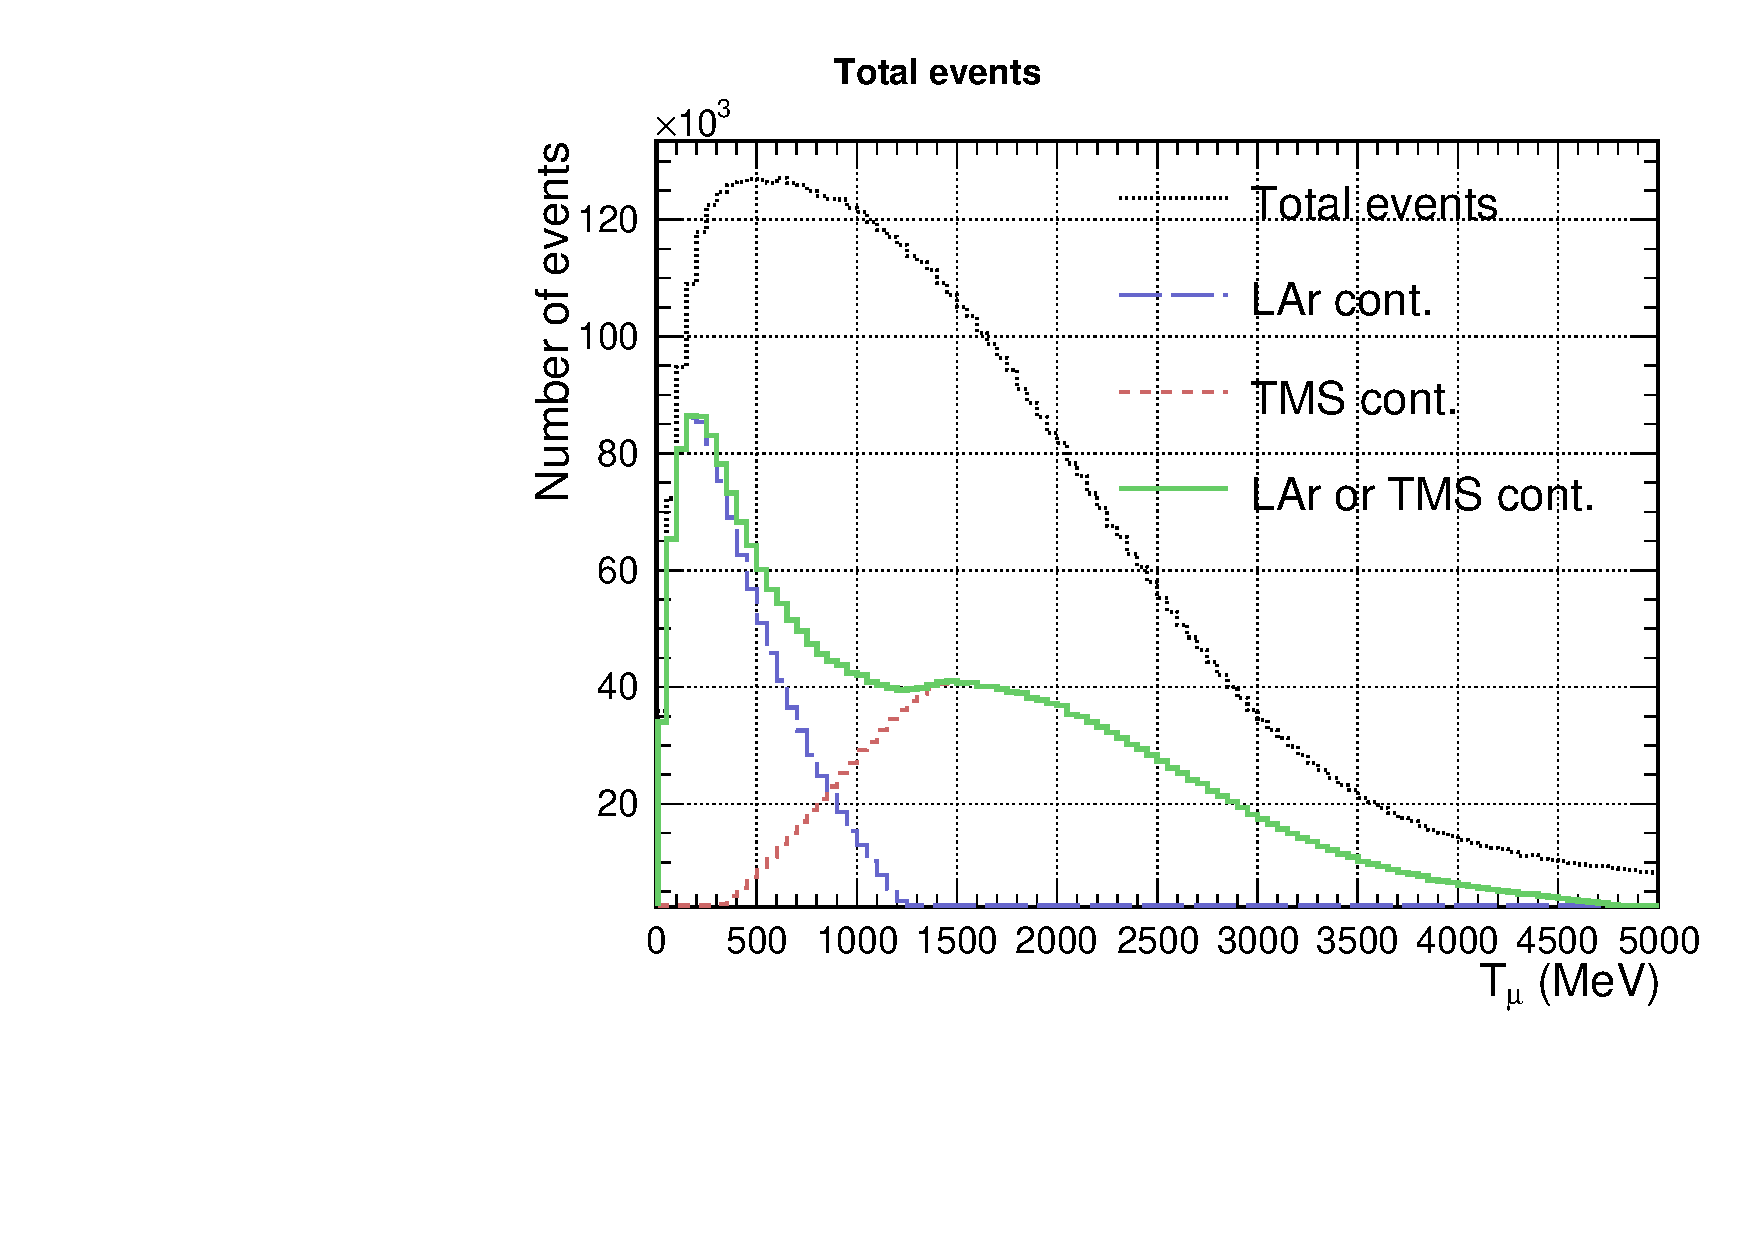
\includegraphics[width=0.49\textwidth, clip, trim={0mm 0mm 0mm 10mm}]{graphics/Simulation/Efficiency/eff_muke.pdf} 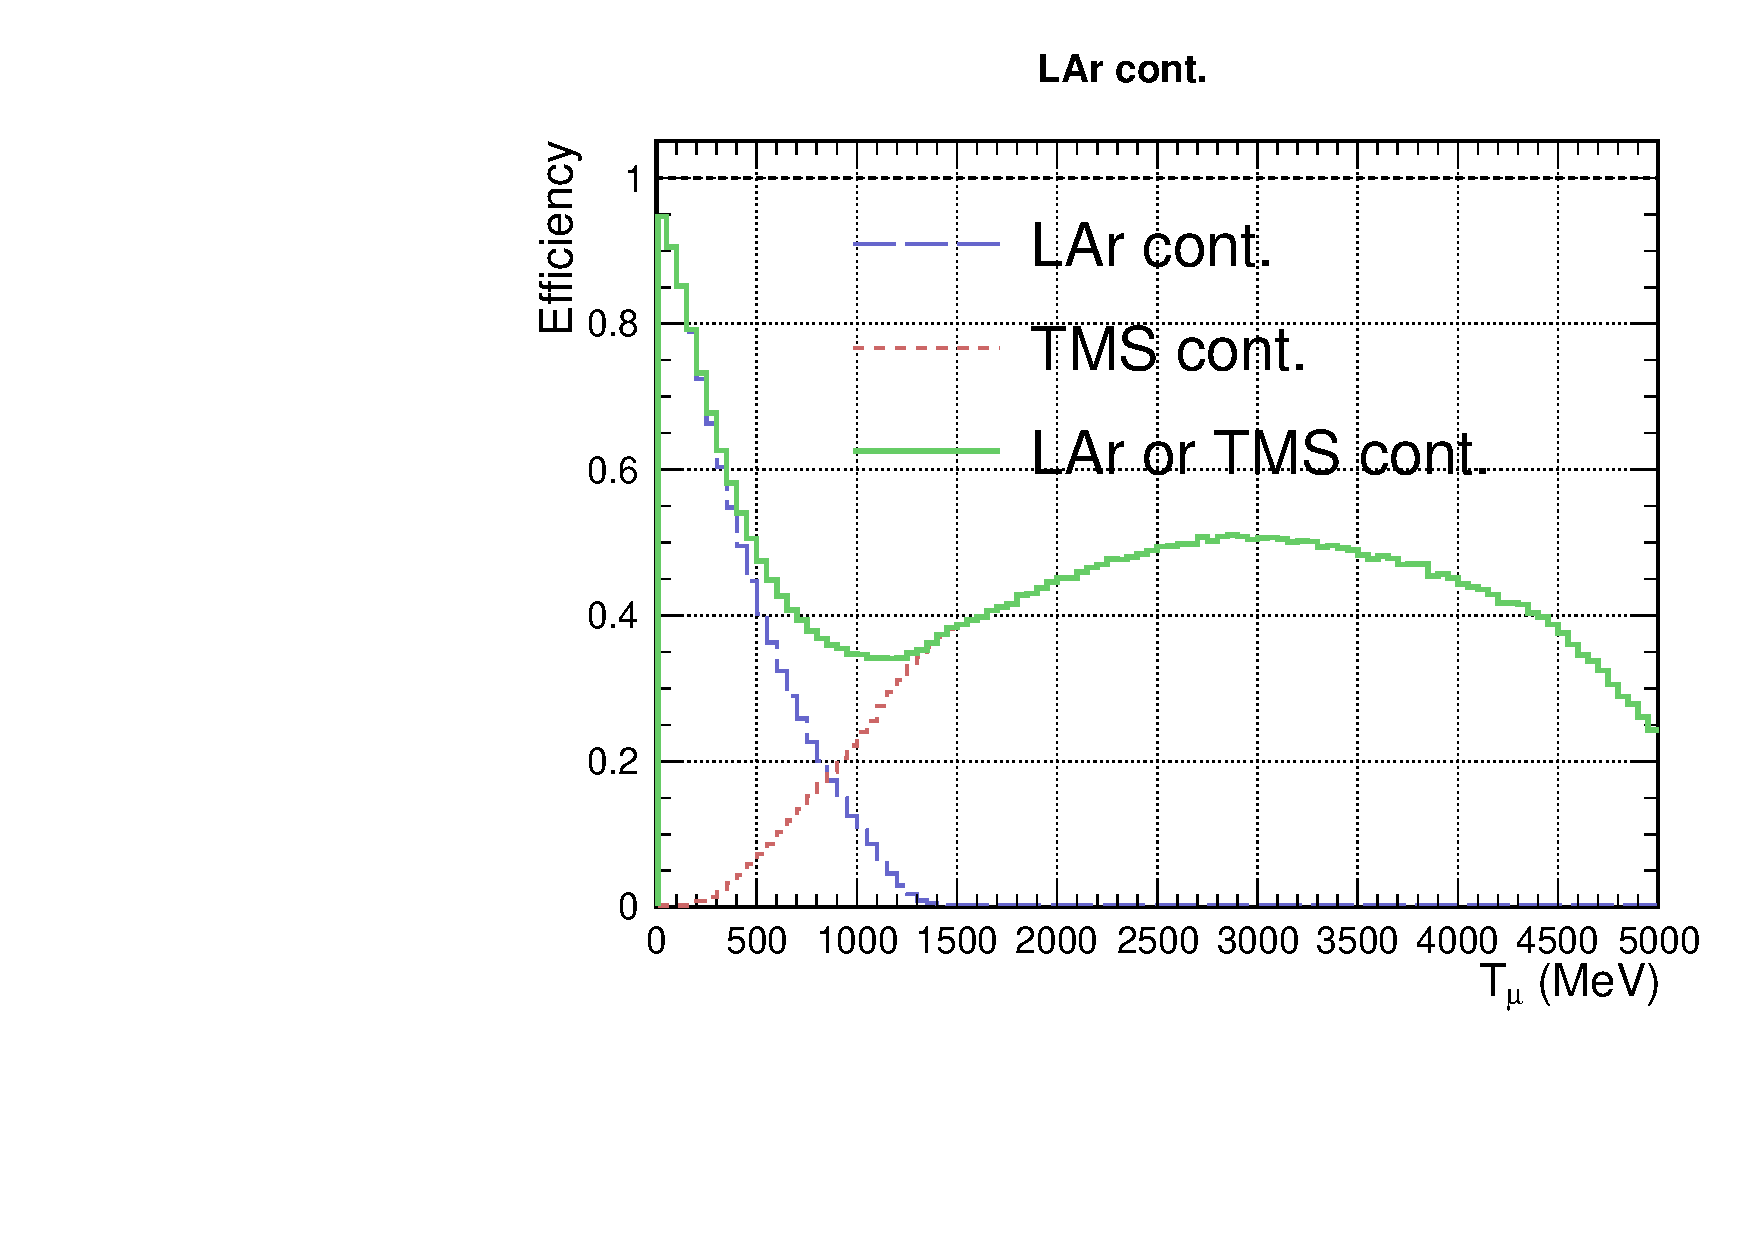
\includegraphics[width=0.49\textwidth, clip, trim={0mm 0mm 0mm 10mm}]{graphics/Simulation/Efficiency/eff_muke_ratio.pdf}
\end{dunefigure}

In Figure \ref{fig:eff_ke_20deg} we additionally include the $\theta_{\nu,\mu}<20\degree$ cut and look at the acceptance in $T_\mu$. The total event distributions shifts considerably to higher energy, now peaking at 2 GeV. The TMS captures the event distribution peak very well, with a flat acceptance of 55\% when $1 < T_\mu < 3 \text{ GeV}$.
% th_mu_nu < 20 deg acceptance in LAr KE
\begin{dunefigure}[]{fig:eff_ke_20deg}
{Efficiency of the LAr, TMS and combined system in $T_\mu$ in the LAr with $\theta_{\nu,\mu}<20\degree$. Left shows the events contained in the different detectors, compared with all events. Right shows the ratio of each category relative the total.}
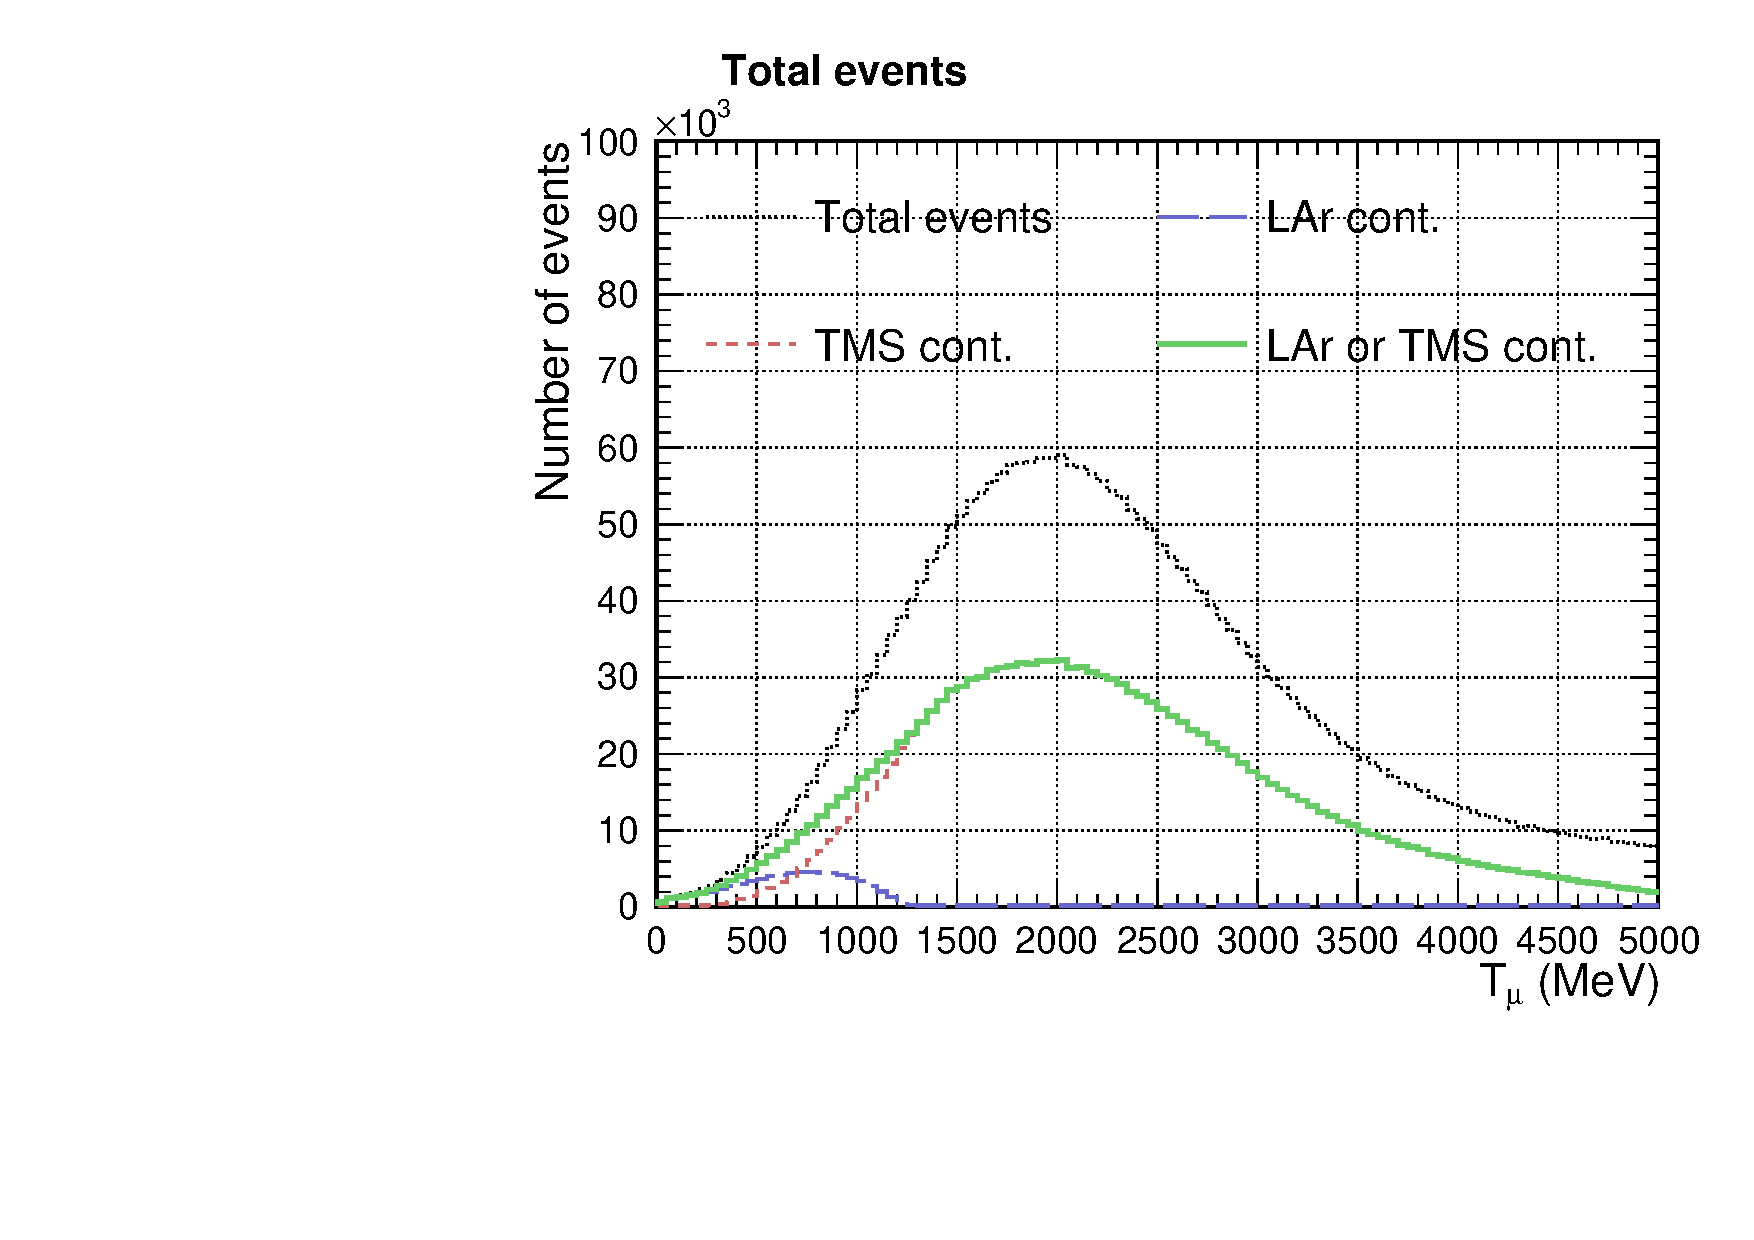
\includegraphics[width=0.49\textwidth, clip, trim={0mm 0mm 0mm 10mm}]{graphics/Simulation/Efficiency/eff_muke_th20.pdf} 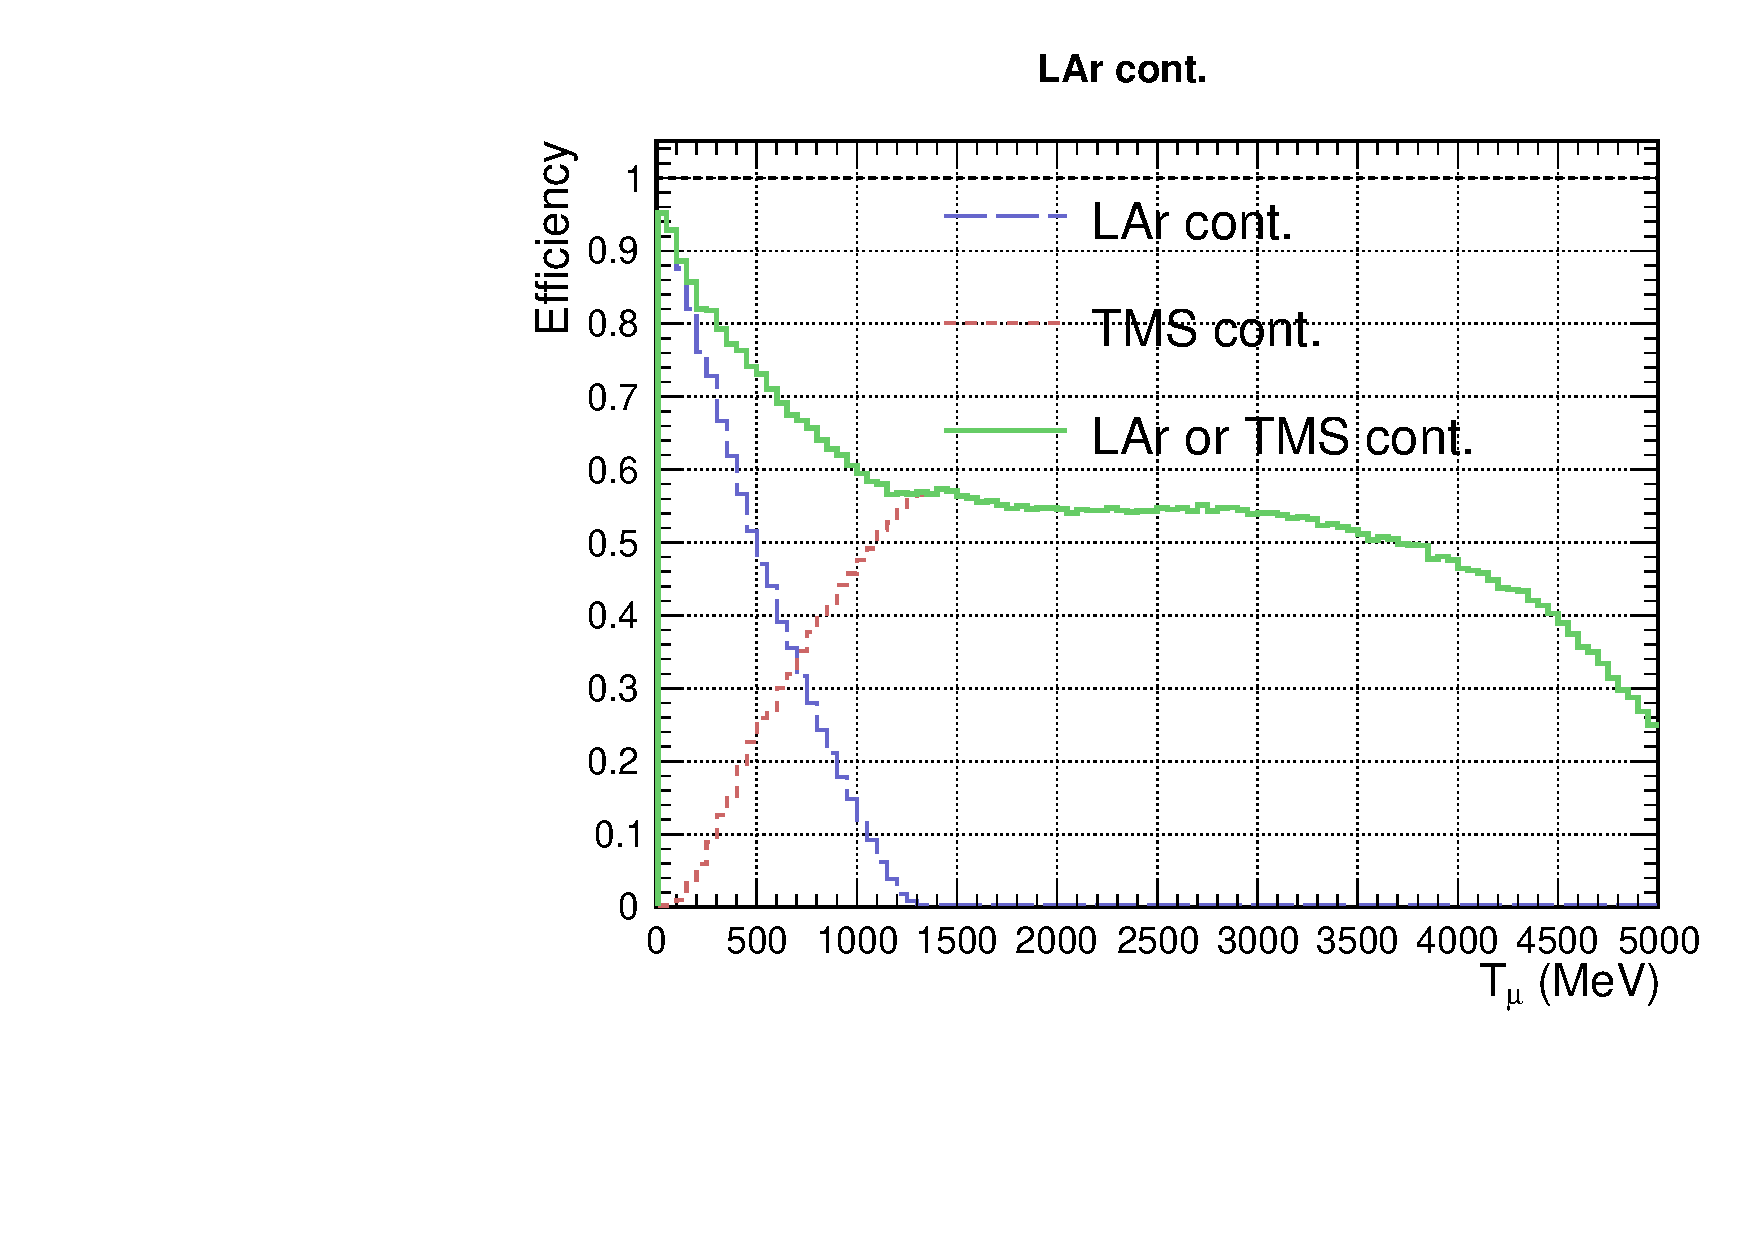
\includegraphics[width=0.49\textwidth, clip, trim={0mm 0mm 0mm 10mm}]{graphics/Simulation/Efficiency/eff_muke_th20_ratio.pdf}
\end{dunefigure}

\subsubsection{Muon Momentum Resolution}
\fixme{Clarence}

Particle trajectories in the \dword{tms} differ substantially from a traditional magnetic spectrumeter. In the TMS, a track's sagitta is, apart from energy loss, independent of momentum: the bend of a track per unit length is inversely proportional to momentum, but its range is proportional. The momentum measurement from the magnetic field is driven not be the magnitude of the sagitta, but by where longitudinally, the sagitta occurs. Consequently, we determine the momentum of the muon via its range - more sensitive on the kinematic regime we operate in - rather than by its curvature.

\subsubsection{Muon Sign Selection}



To study the bending of tracks in the TMS we use the $x-z$ view to look for deviations from a straight line. The method draws a straight line between the LAr start and endpoint, alternatively the LAr endpoint and the TMS start point, and projects it to the $z$ of the last hit of the track. This provides an estimate of the last hit position if it traversed in a straight line. If the last hit is above the the expected, the candidate is expected to have positive charge, and vice verse for negative charge. The procedure is outlined in Figure \ref{fig:bend_method}. It is important to stress that the full reconstruction will \emph{not} use such a method, and will instead fit particle hypotheses. The choice of sign selection metric presented was chosen because it requires minimal reconstruction, so can be done early in the TMS design process to gauge performance.
\begin{dunefigure}[]{fig:bend_method}
{An example event display showing the method for calculating the ``signed distance'' metric for determining charge of the particle in the magnetic field in the truth studies.}
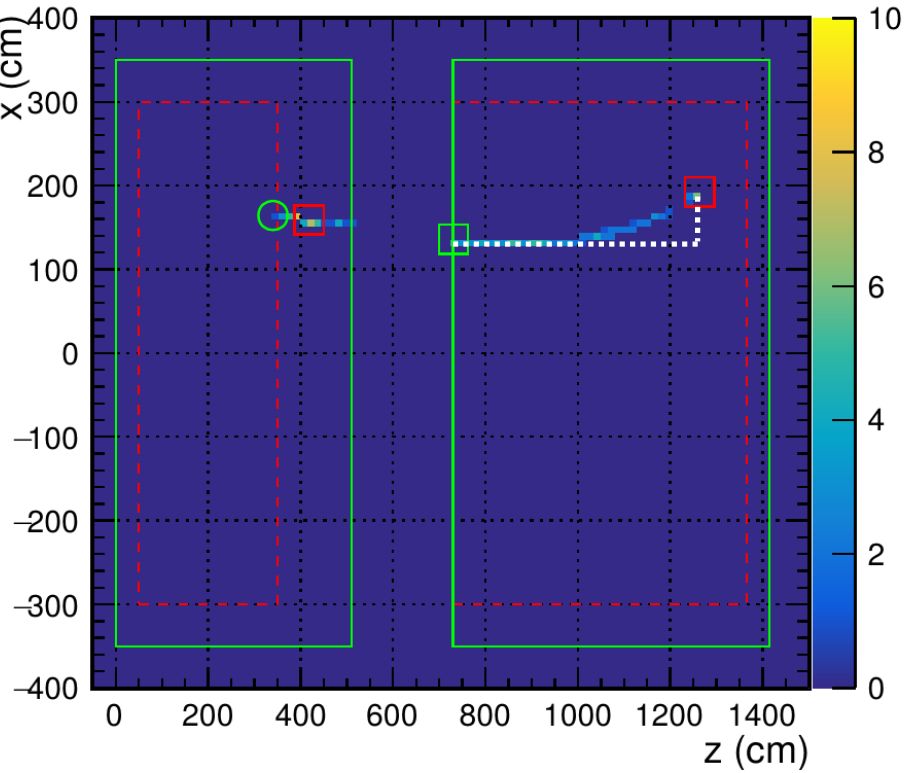
\includegraphics[width=0.49\textwidth]{graphics/Simulation/Bend/Bend_Estimate.png}
\end{dunefigure}

The equation derived for the ``signed distance'' is
% Use Clarence's updated signed distance instead?
\begin{equation}
    %SD = \frac{(x_2-x_1) z_3 + x_1 z_2 - z_1 x_2 -(z_2-z_1)x_3}{\sqrt{(x_2-x_1)^2+(z_2-z_1)^2}}
    SD = (x_3-x_1) - (x_2-x_1)\frac{z_3-z_1}{z_2-z_1}
\end{equation}
where $x_{1,2,3},z_{1,2,3}$ is the $x,z$ position of the LAr exit point (or LAr start point), TMS entry point (or LAr exit point), and the last hit in the TMS respectively.

Figure \ref{fig:bend_results} shows the ``signed distance'' metric for the generated forward horn current sample. This study only uses tracks in the center region to avoid the ``double-bending'' tracks in the upper module, and the changing in bending direction in the lower module.

\begin{dunefigure}[]{fig:bend_results}
{The ``signed distance'' metric for determining the charge of the track from its bending. The success rate is tabulated in 
Table \ref{tab:muon_bend} for $\mu^-$ and $\mu^+$.}
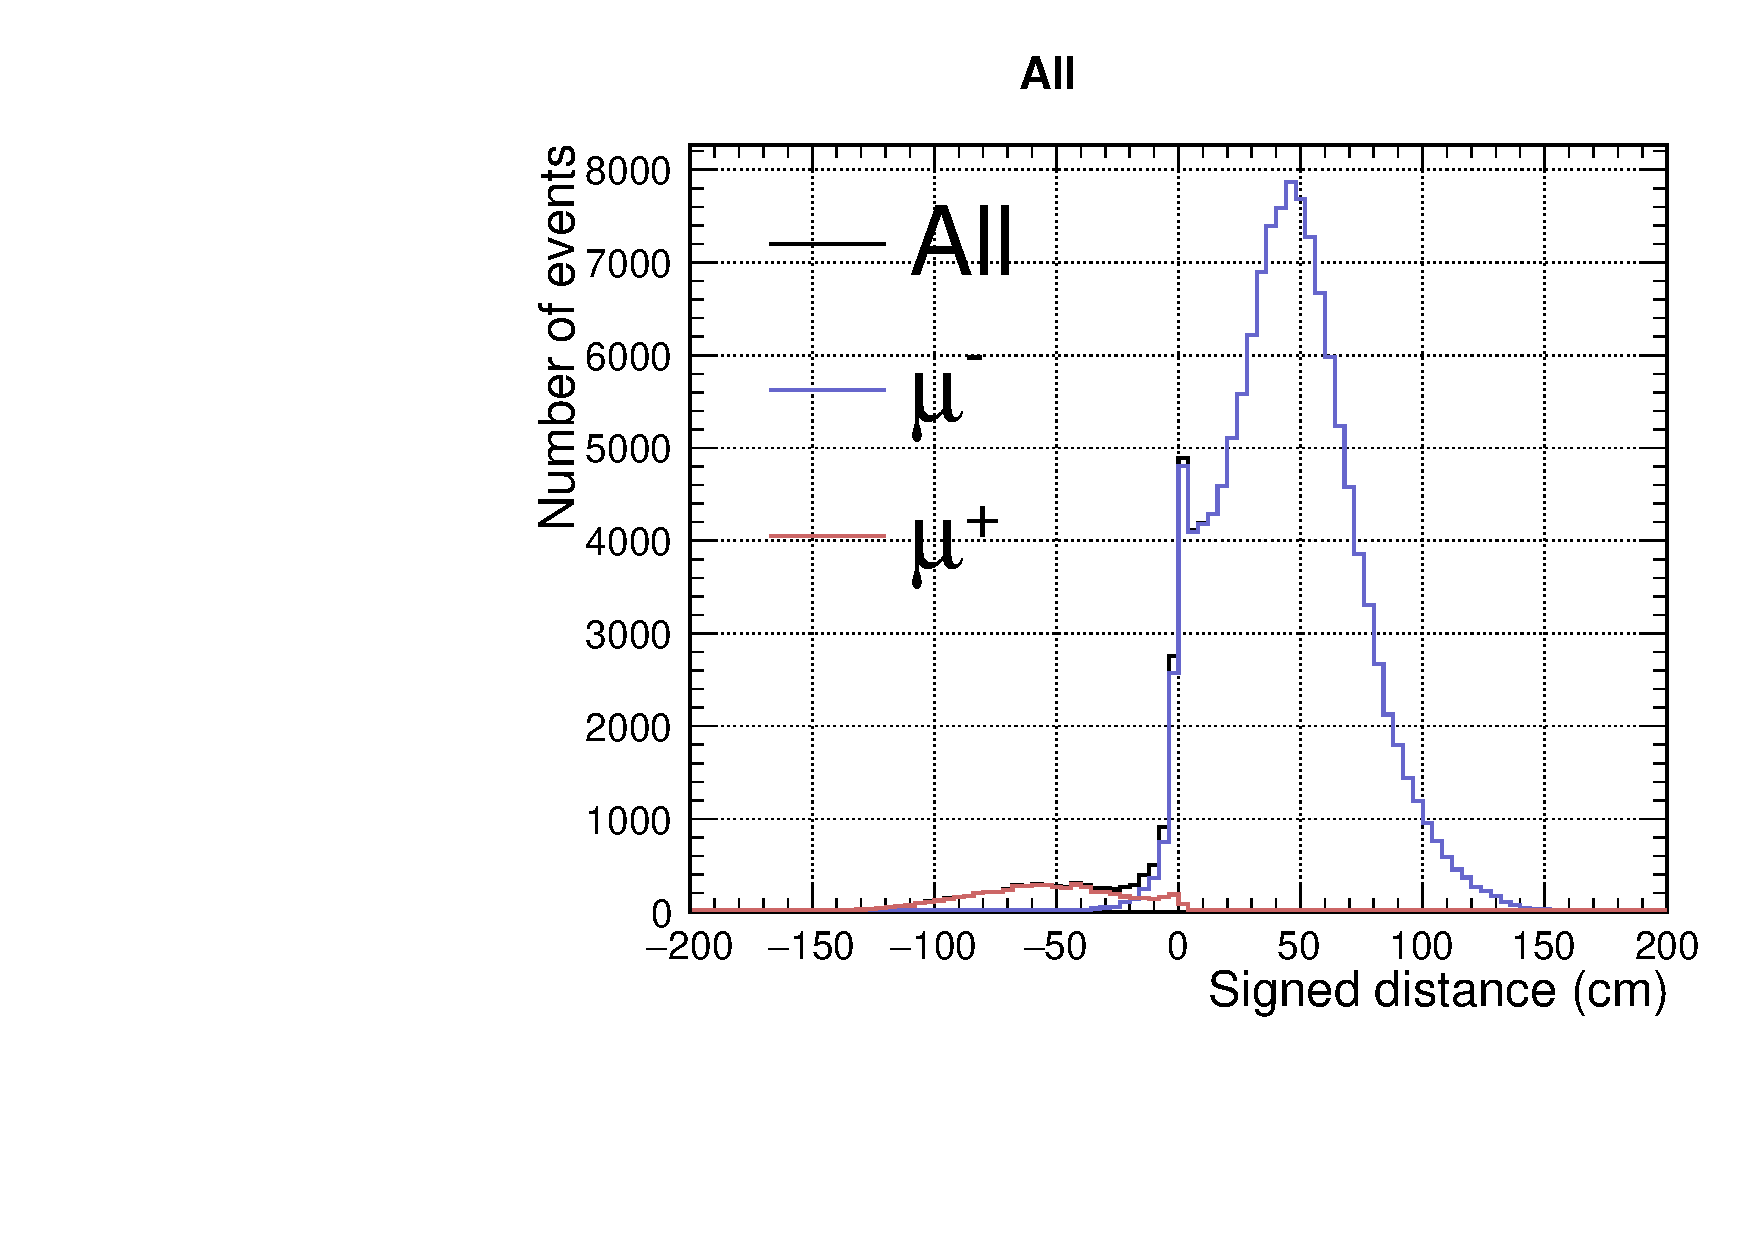
\includegraphics[width=0.65\textwidth, clip, trim={0mm 0mm 0mm 10mm}]{graphics/Simulation/Bend/cmetric_signed_distance.pdf}
\end{dunefigure}

The results from Figure \ref{fig:bend_results} are tabulated in Table \ref{tab:muon_bend}. Firstly, we note the peaks at $\pm50\text{ cm}$, meaning the contained muons on average bend 50 cm in the modules. We observe a mis-identification rate of 3.4 and 1.9\% for $\mu^-$ and $\mu^+$ respectively in FHC. Figures \ref{fig:bend_results_mum} and \ref{fig:bend_results_mup} show that the mis-identification of the lepton charge predominantly happens when the TMS entrance kinetic energy is below 500 MeV. If a requirement is made on the TMS entrance kinetic energy at 500 MeV, the $\mu^-$ mis-identification rate falls to 0.8\%, and at 1 GeV it is 0.3\%; for $\mu^+$ the mis-identification rate falls to 0.4\% and 0.2\%.

% These are using Clarence's metric
\begin{dunetable}
[]
{cccc}
{tab:muon_bend}
{Fraction of events with their calculated signed distance for $\mu^{\pm}$ in the TMS, with cuts on true kinetic energy included. The fractions can be deduced from Figures \ref{fig:bend_results_mum} and \ref{fig:bend_results_mup}.}
Particle & Signed Distance & $T^{TMS}_\mu$ & Fraction \\ \toprowrule
$\mu^-$ & $SD>0$ & --- & 96.6\% \\ \colhline
$\mu^-$ & $SD<0$ & --- & 3.4\% \\ \colhline
$\mu^-$ & $SD>0$ & $> 0.5 \text{ GeV}$ & 99.2\% \\ \colhline
$\mu^-$ & $SD<0$ & $> 0.5 \text{ GeV}$ & 0.8\% \\ \colhline
$\mu^-$ & $SD>0$ & $> 1.0 \text{ GeV}$ & 99.7\% \\ \colhline
$\mu^-$ & $SD<0$ & $> 1.0 \text{ GeV}$ & 0.3\% \\ \colhline \colhline 
$\mu^+$ & $SD>0$ & --- & 1.9\% \\ \colhline
$\mu^+$ & $SD<0$ & --- & 98.1\% \\ \colhline
$\mu^+$ & $SD>0$ & $> 0.5 \text{ GeV}$ & 0.4\% \\ \colhline
$\mu^+$ & $SD<0$ & $> 0.5 \text{ GeV}$ & 99.6\% \\ \colhline
$\mu^+$ & $SD>0$ & $> 1.0 \text{ GeV}$ & 0.2\% \\ \colhline
$\mu^+$ & $SD<0$ & $> 1.0 \text{ GeV}$ & 99.8\% \\ 
% no \colhline on final row
\end{dunetable}

\begin{dunefigure}[]{fig:bend_results_mum}
{The true TMS entrance muon kinetic energy for $\mu^-$ with positive and negative signed distance. The wrongly assigned signed distance ($SD<0$ for $\mu^-$) happens predominantly at low muon kinetic energy, and is mostly gone by 1 GeV.}
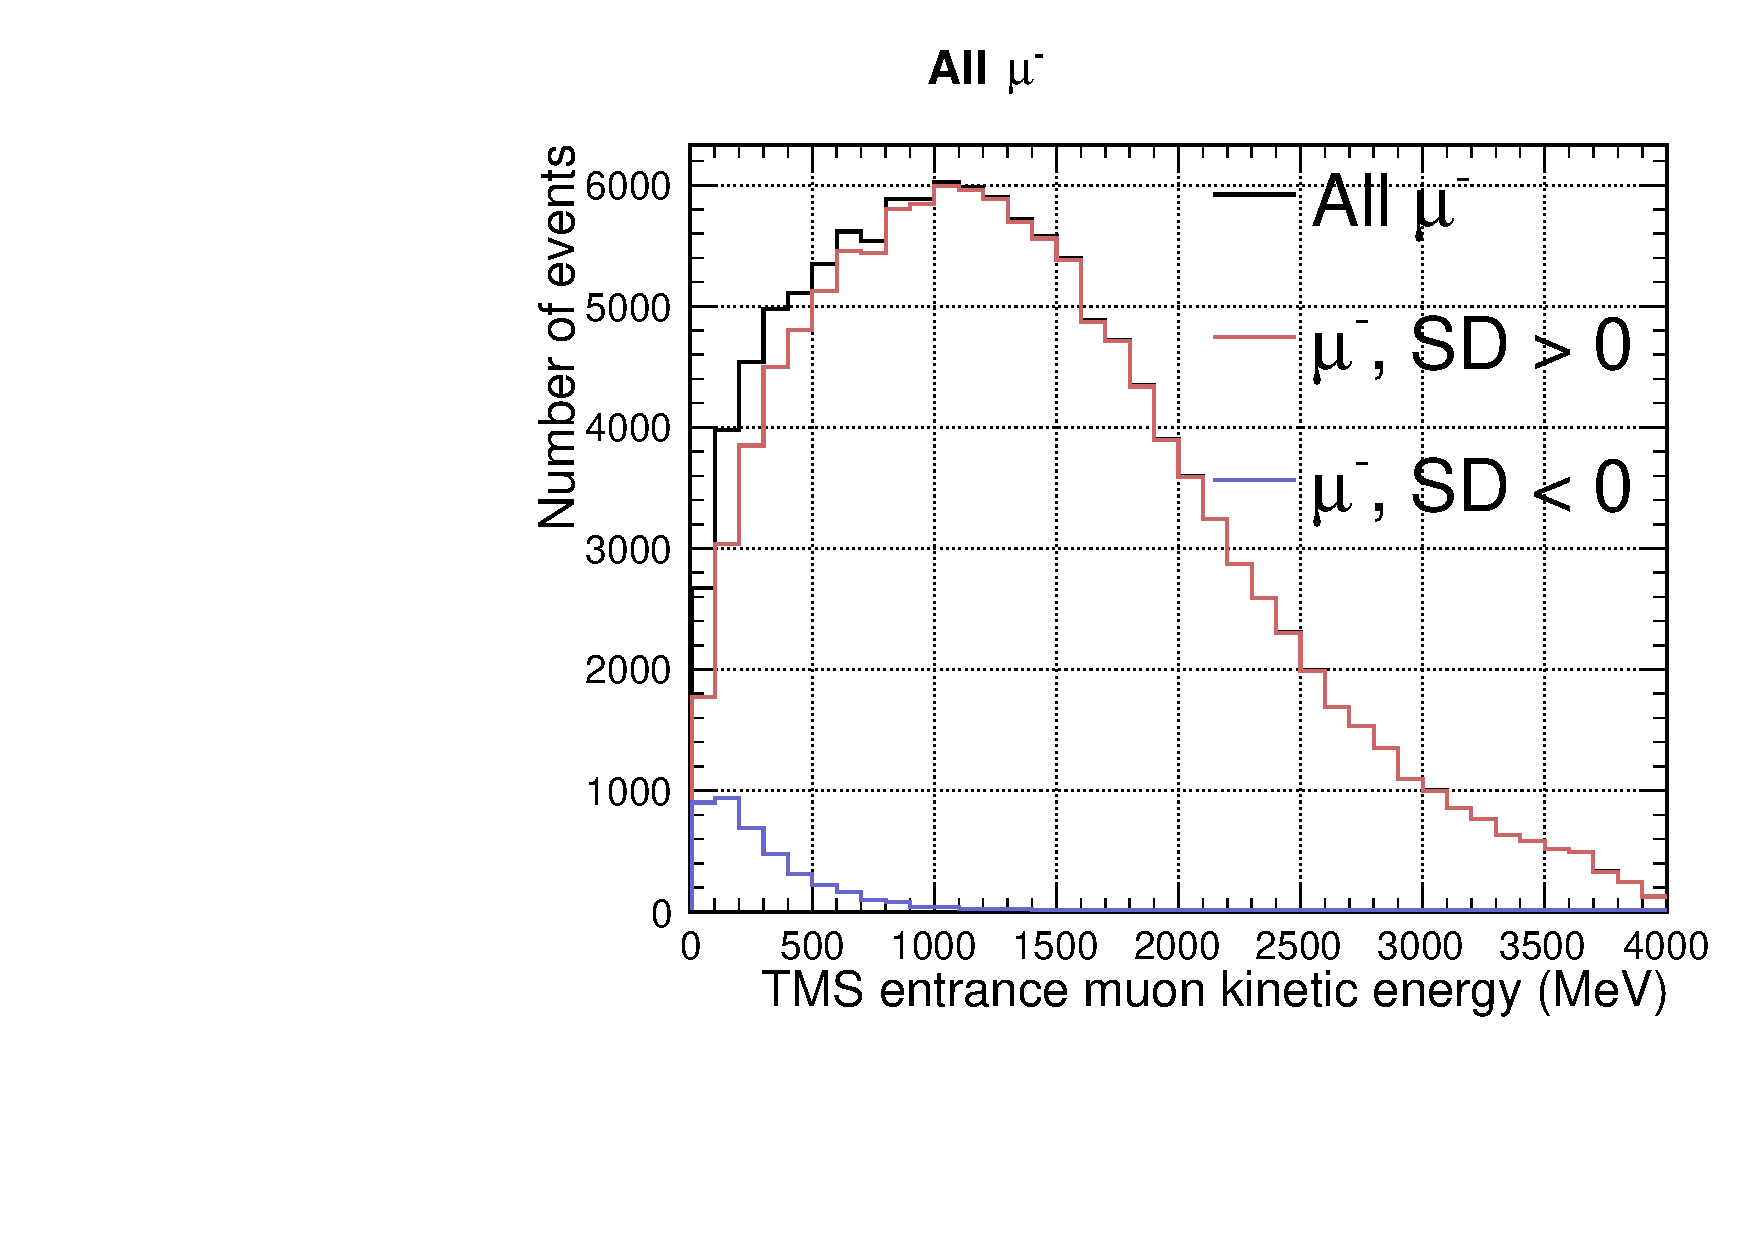
\includegraphics[width=0.49\textwidth, clip, trim={0mm 0mm 0mm 10mm}]{graphics/Simulation/Bend/cmetric_signed_distance_KE.pdf} 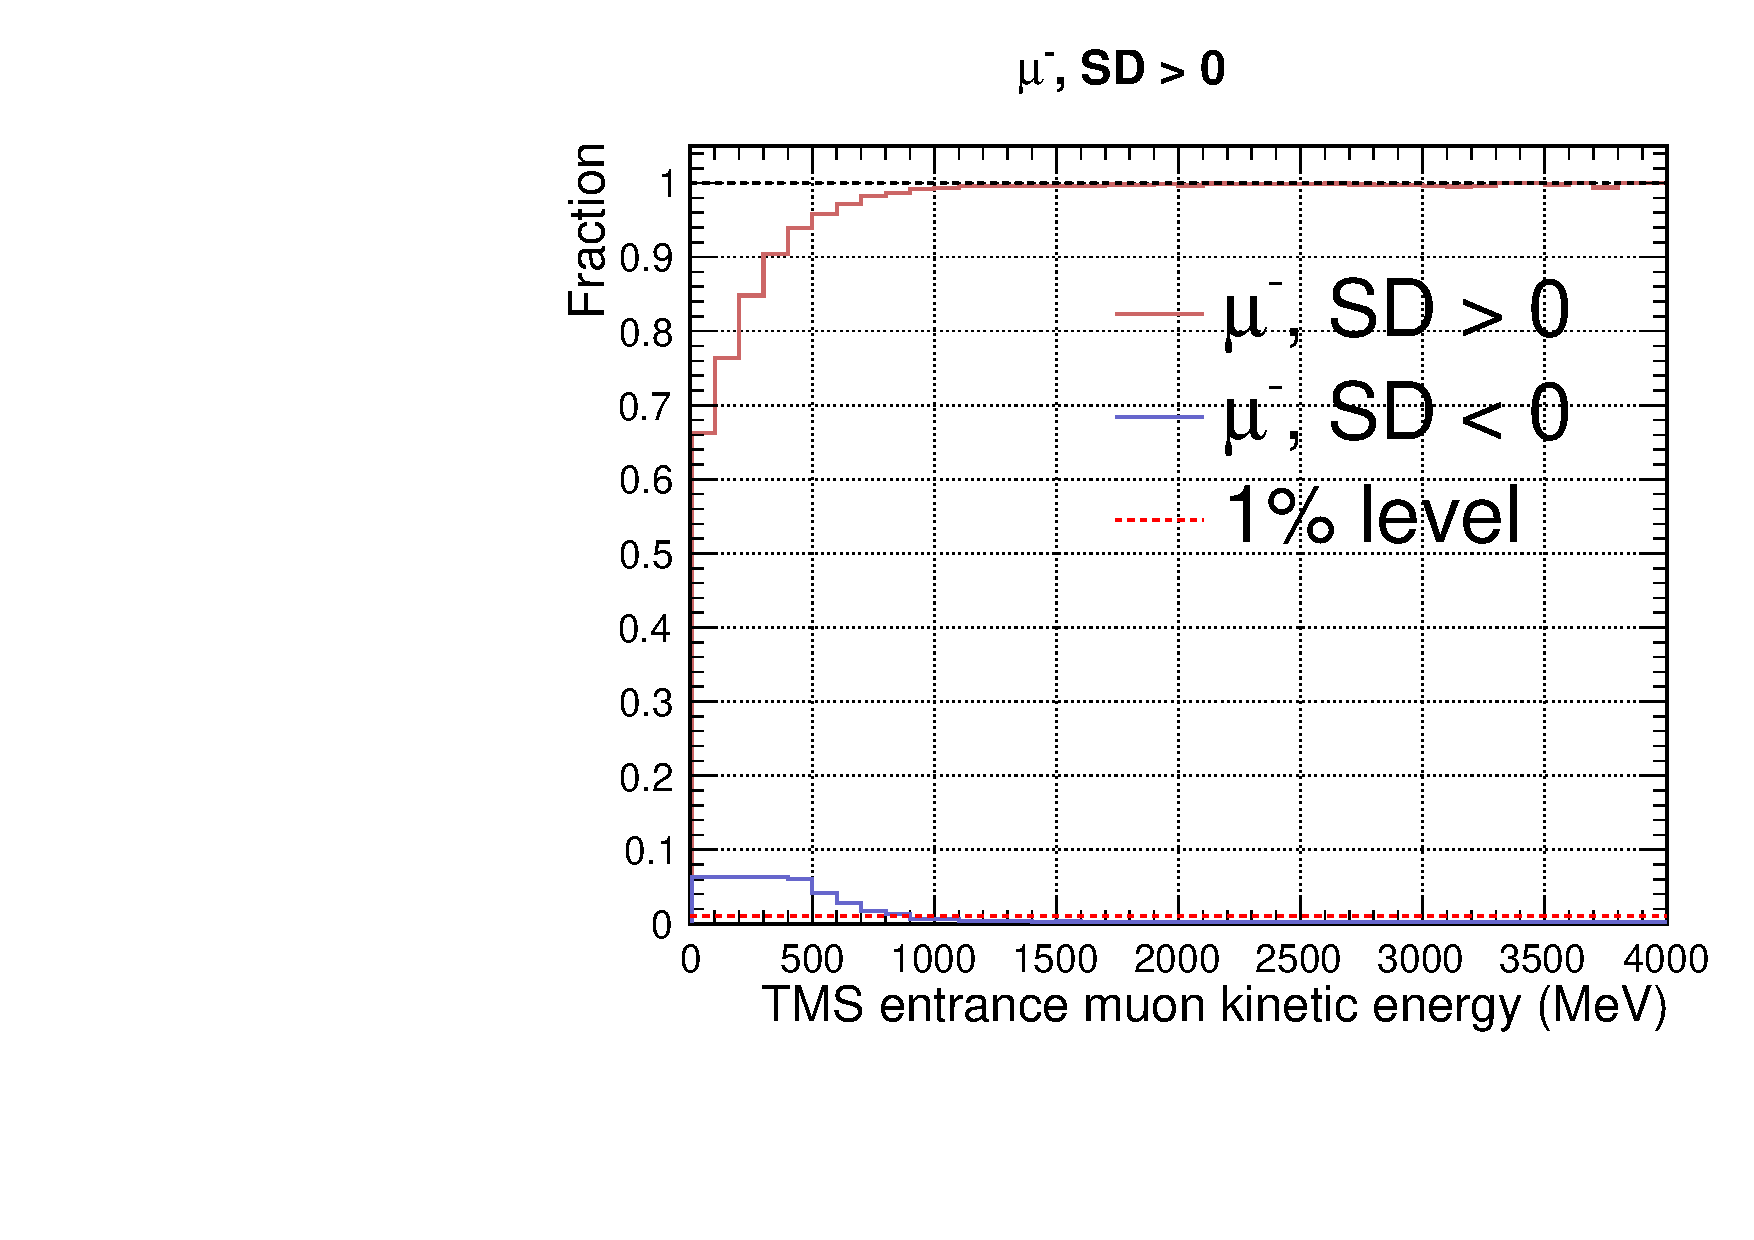
\includegraphics[width=0.49\textwidth, clip, trim={0mm 0mm 0mm 10mm}]{graphics/Simulation/Bend/cmetric_signed_distance_KE_ratio.pdf}
\end{dunefigure}

\begin{dunefigure}[]{fig:bend_results_mup}
{The true TMS entrance muon kinetic energy for $\mu^+$ in FHC with positive and negative signed distance. The wrongly assigned signed distance ($SD>0$ for $\mu^+$) happens predominantly at low muon kinetic energy, and is mostly gone by 500 MeV.}
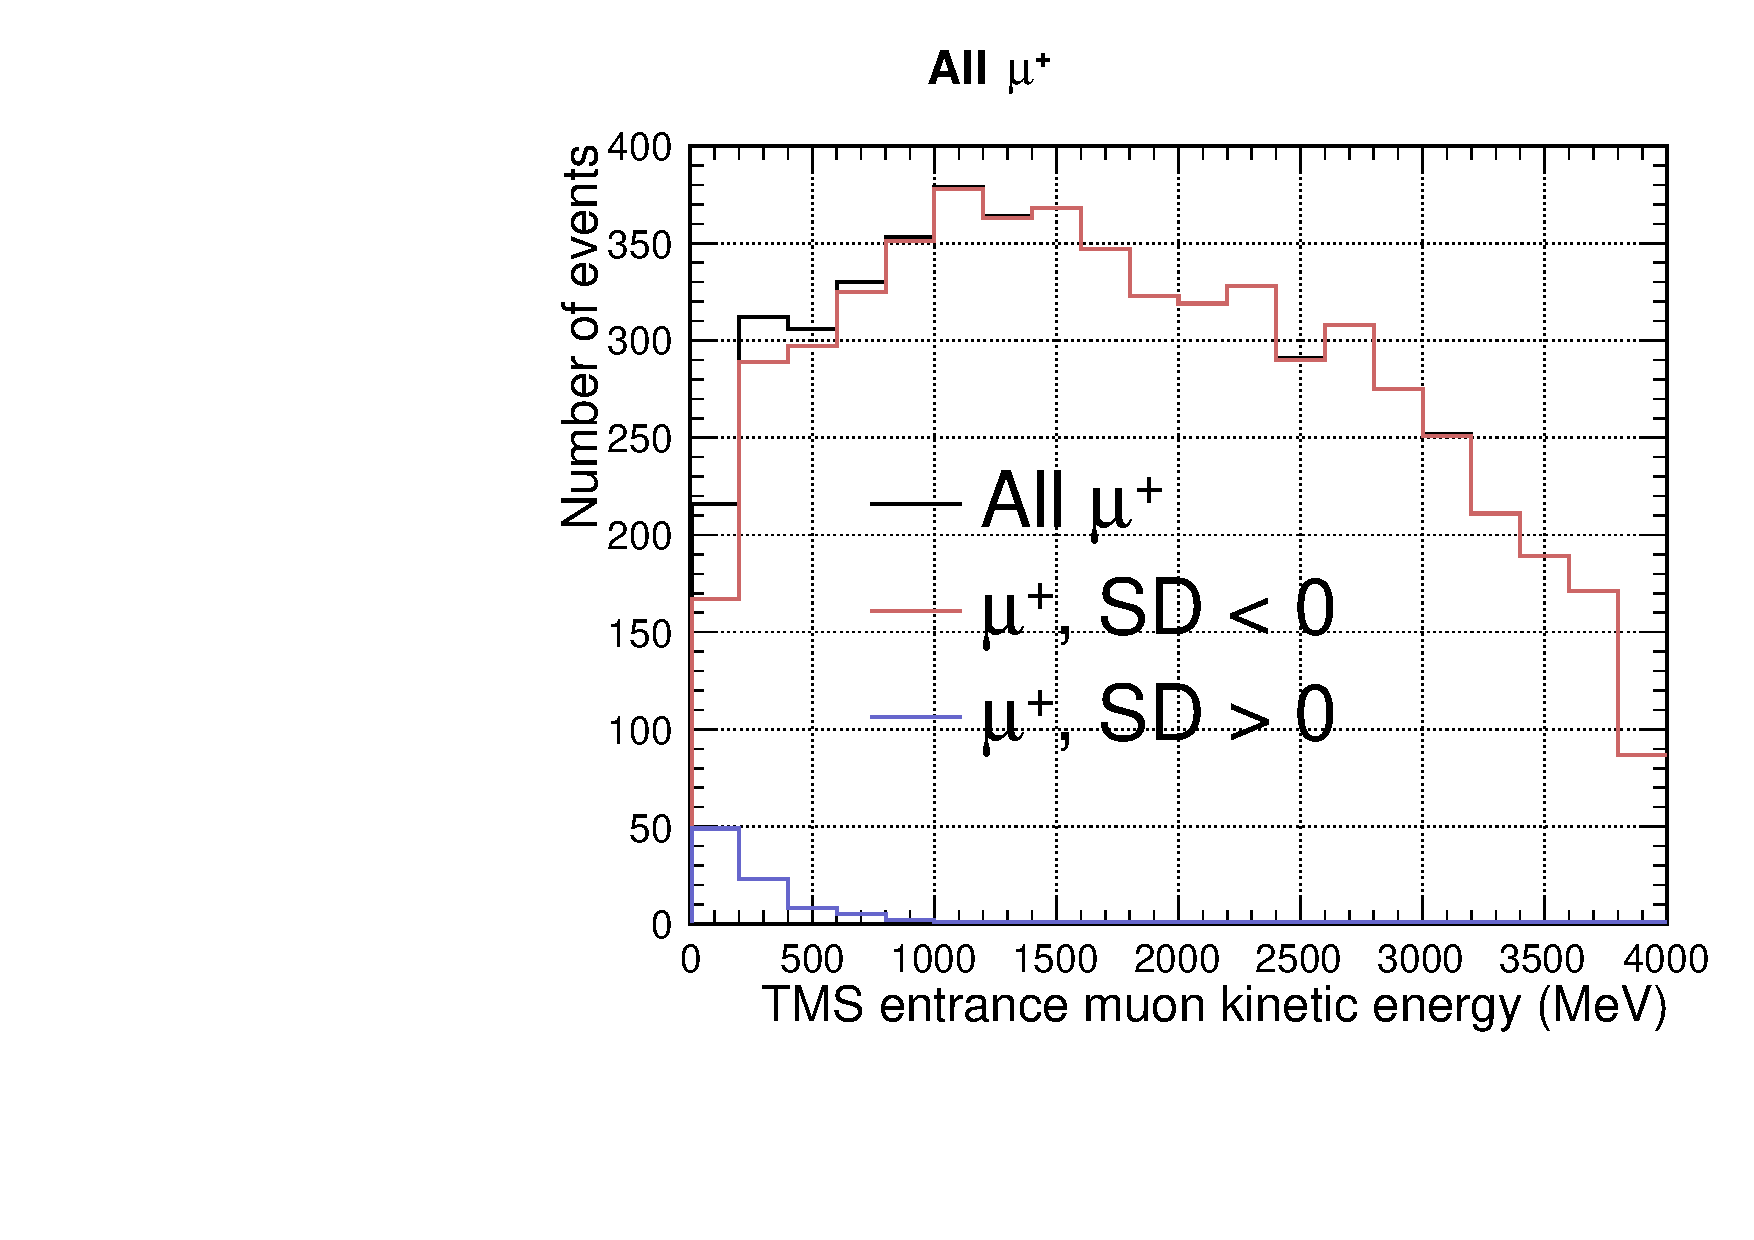
\includegraphics[width=0.49\textwidth, clip, trim={0mm 0mm 0mm 10mm}]{graphics/Simulation/Bend/cmetric_signed_distance_KE_muplus.pdf} 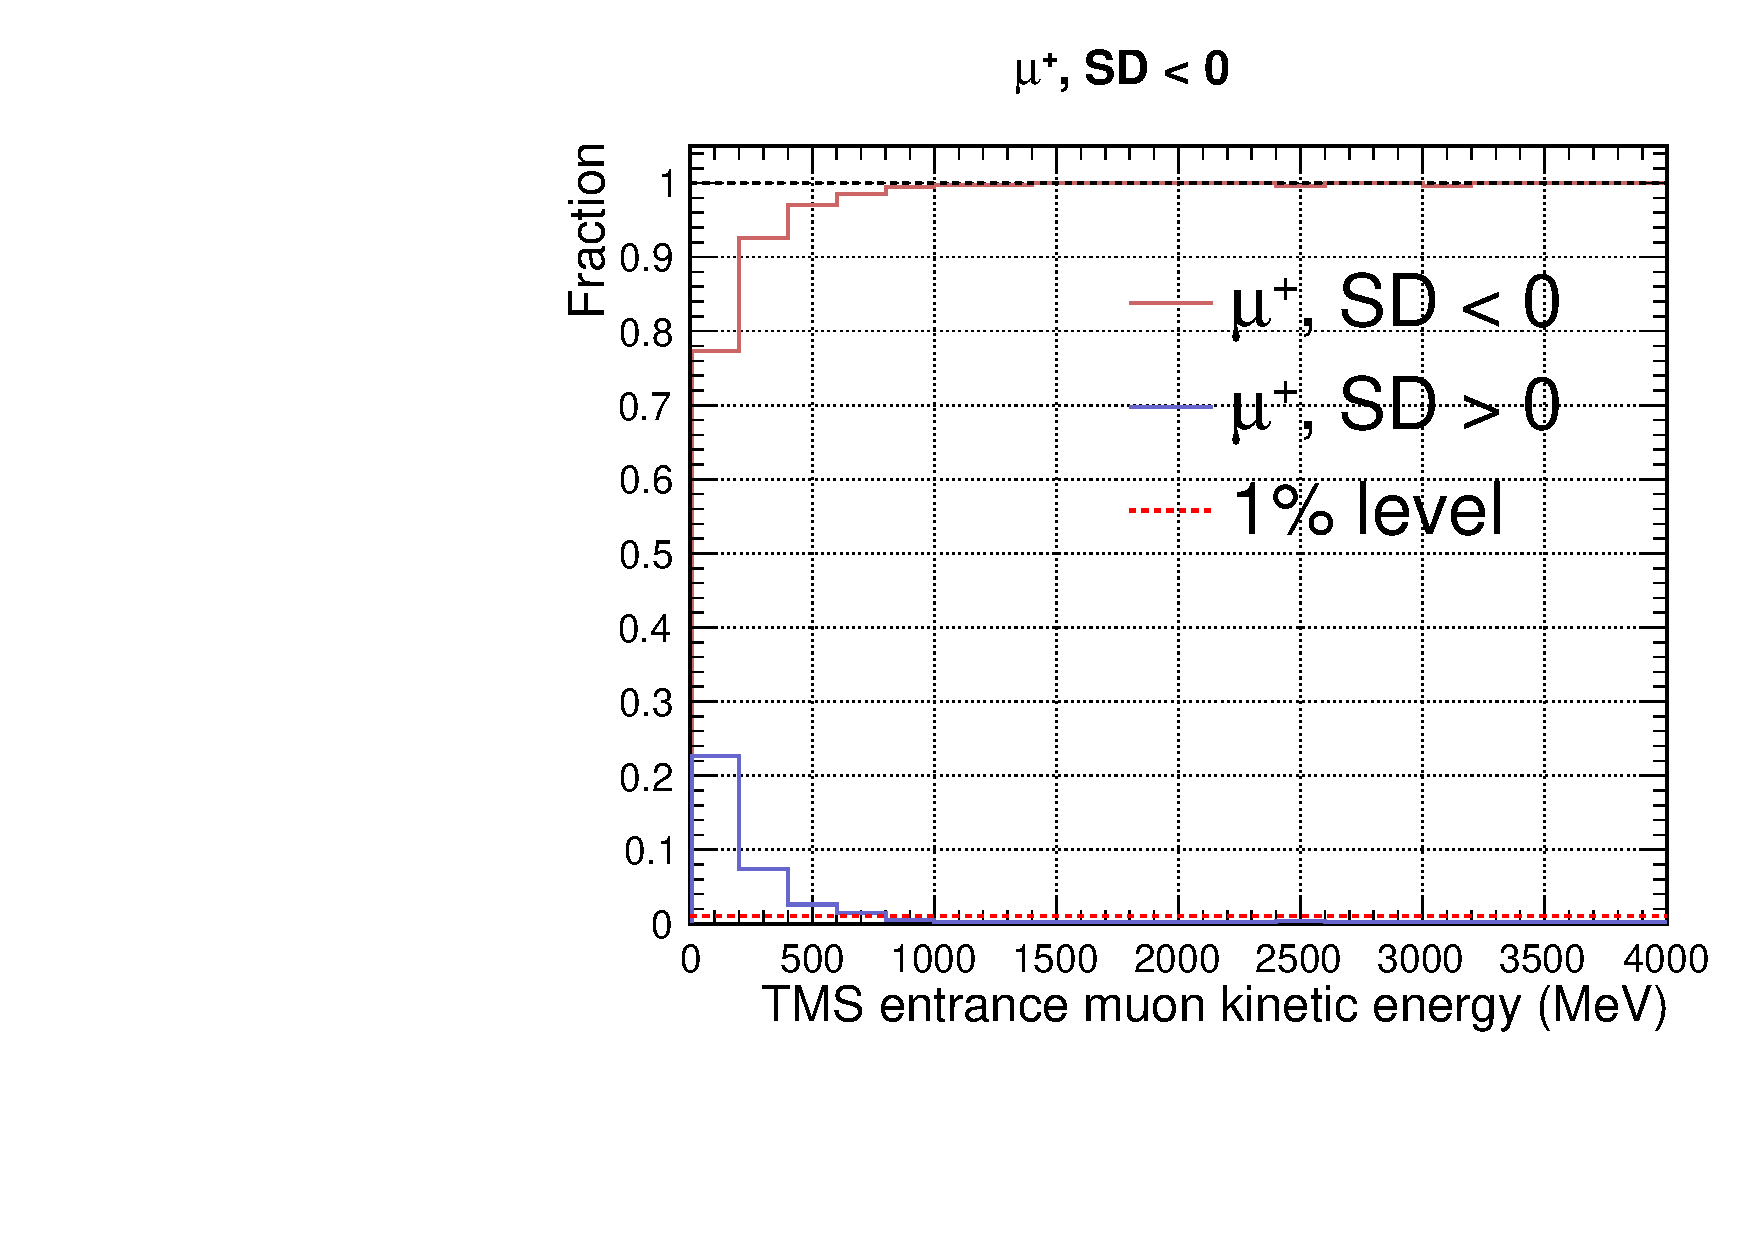
\includegraphics[width=0.49\textwidth, clip, trim={0mm 0mm 0mm 10mm}]{graphics/Simulation/Bend/cmetric_signed_distance_KE_muplus_ratio.pdf}
\end{dunefigure}

% These are using Gavin's signed distance metric
\iffalse
\begin{dunetable}
[]
{cccc}
{tab:muon_bend}
{Fraction of events with their calculated signed distance for $\mu^{\pm}$ in the TMS, including the effects of cuts on the true kinetic energy in the TMS.}
Particle & Signed Distance & $T^{TMS}_\mu$ & Fraction \\ \toprowrule
$\mu^-$ & $SD>0$ & & 95.4\% \\ \colhline
$\mu^-$ & $SD<0$ & & 4.6\% \\ \colhline
$\mu^-$ & $SD>0$ & $> 0.5 \text{ GeV}$ & 98.0\% \\ \colhline
$\mu^-$ & $SD<0$ & $> 0.5 \text{ GeV}$ & 2.0\% \\ \colhline
$\mu^-$ & $SD>0$ & $= 1.0 \text{ GeV}$ & 99.1\% \\ \colhline
$\mu^-$ & $SD<0$ & $= 1.0 \text{ GeV}$ & 0.9\% \\ \colhline
$\mu^+$ & $SD>0$ & & 4.0\% \\ \colhline
$\mu^+$ & $SD<0$ & & 96.0\% \\ % no \colhline on final row
\end{dunetable}
\fi


\label{sec:tms-ovvw-perf}
%%%%%%%%%%%%%%%%%%%%%%%%%%%%%%%%
\subsubsection{Progress toward Reconstruction}
\label{sec:tms-ovvw-perf}
The TMS reconstruction is in progress, and is inspired from reconstruction in the similarly designed MINOS and (Baby-)MIND detectors. The current approach is investigating running the track finding and reconstruction simultaneously through a Kalman filter, or having a separate track finding algorithm identify track candidates which it feeds to the Kalman track reconstruction.

Once formalised, the LAr reconstruction will provide track candidates which escape the ArgonCube volume. Those candidates are propagated through the gap region, accounting for energy loss and multiple scattering. This can then provide either a seed for the TMS track finding and reconstruction, or be matched against the track candidates from the stand-alone TMS track finding and reconstruction.

\subsubsubsection{Track finding}
For the track finding stage, we are currently investigating three approaches. They all run in each view separately, and the 2D to 3D track matching and merging is done at a later stage.

\begin{itemize}
    \item Perform a Hough transform in each view separately, and find which hits intersect the primary Hough line. Traverse the hits and group neighbouring hits into a track candidate. Take remaining hits (not belonging to a candidate) and repeat process to see if there is a $N^{th}$ track candidate. Hough transform only up to transition layer in $y-z$ view and full range in $x-z$ view due to bending in the $y-z$ view becoming strong (not straight lines) after transition layer. Hence the Hough transform is often more successful in the $x-z$ view, and the neighbour clustering in $y-z$ is critically important.

    \item Sort the hits ascending in $z$, and run a custom A* path finding algorithm from first to last hit in $z$. The intent is to find the shortest path between the first and last hit, only traversing cells that have been hit. If no path is found from start to finish, repeat A* path finding running until the hit with second largest z, and continue.
    
    \item Sort the hits ascending in $z$, and run a Kalman filter from first to last hit in $z$. For this to succeed, the Kalman filter needs to account for the energy-loss, bending and multiple-scattering happening in the iron and scintillator layers. 
\end{itemize}

The track finding will benefit from $y-z$ and $x-z$ views communicating to correctly identify particles based on their range in z, for instance making sure the longest track candidate has similar start and end positions in both views. This is particularly useful to find the endpoint of a track in $y-z$ using the $x-z$ view, since the end of a track in $y-z$ is often bent significantly due to the magnetic field. 

We envisage using bifurcations in track candidates to tag non-muons (as muons rarely undergo secondary interactions, compared to pions), and split candidates into separate track candidates if the bifurcation is $N$ planes long.

One of the track finding algorithms (Hough transform followed by adjacent merging) is shown in Figure \ref{fig:track_Hough_1} for two single-track events. These are particularly difficult single-track events as they traverse the gap region so have discontinuities in both views. The Hough transform correctly identifies the dominant straight line hits of the track, and the subsequent neighbour clustering finds the hits across the gap regions.
\begin{dunefigure}[]{fig:track_Hough_1}
{Two single-track events in the TMS, where tracks are found by the Hough+clustering algorithm, showing $x-z$ (left) and $y-z$ (right) hits. The green and red boxes show the total and fiducial volume respectively, the vertical gray line shows the region where the TMS transitions from thin to thick iron layers, and the three horizontal white dotted regions in the $x-z$ view shows the gap region. The yellow fills show the hits that were found by the procedure. The $x-z$ view shows the tracks traversing the central and lower gap region respectively, leaving a broken track in both views. Despite this, the Hough transform and adjacent hit merging finds all relevant hits in the track. N.B. the detector coordinate system differs from the event displays by being in mm (not cm) and translated by $\{x,y,z\}=\{0, 5, 411\}$ mm. }
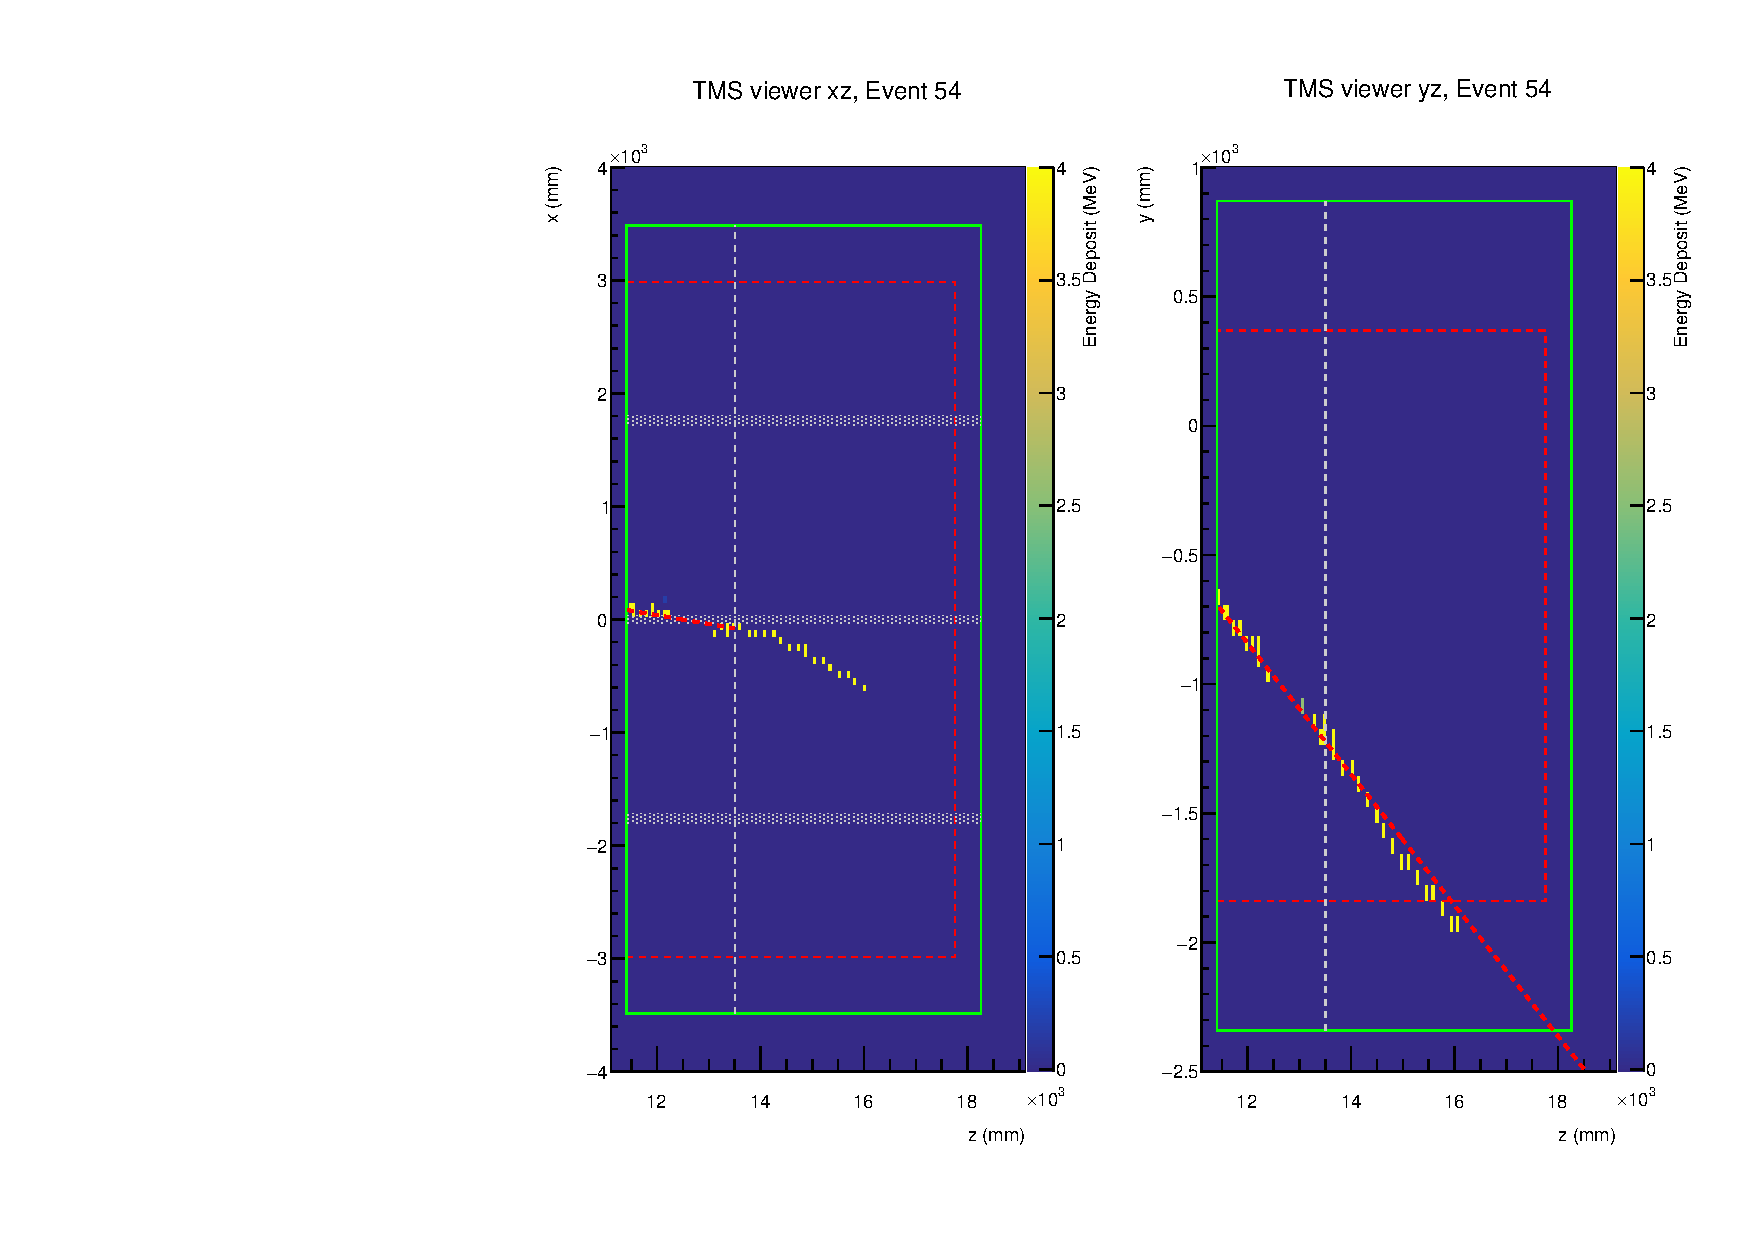
\includegraphics[width=0.49\textwidth]{graphics/Simulation/Hough/Hough_Example.pdf} 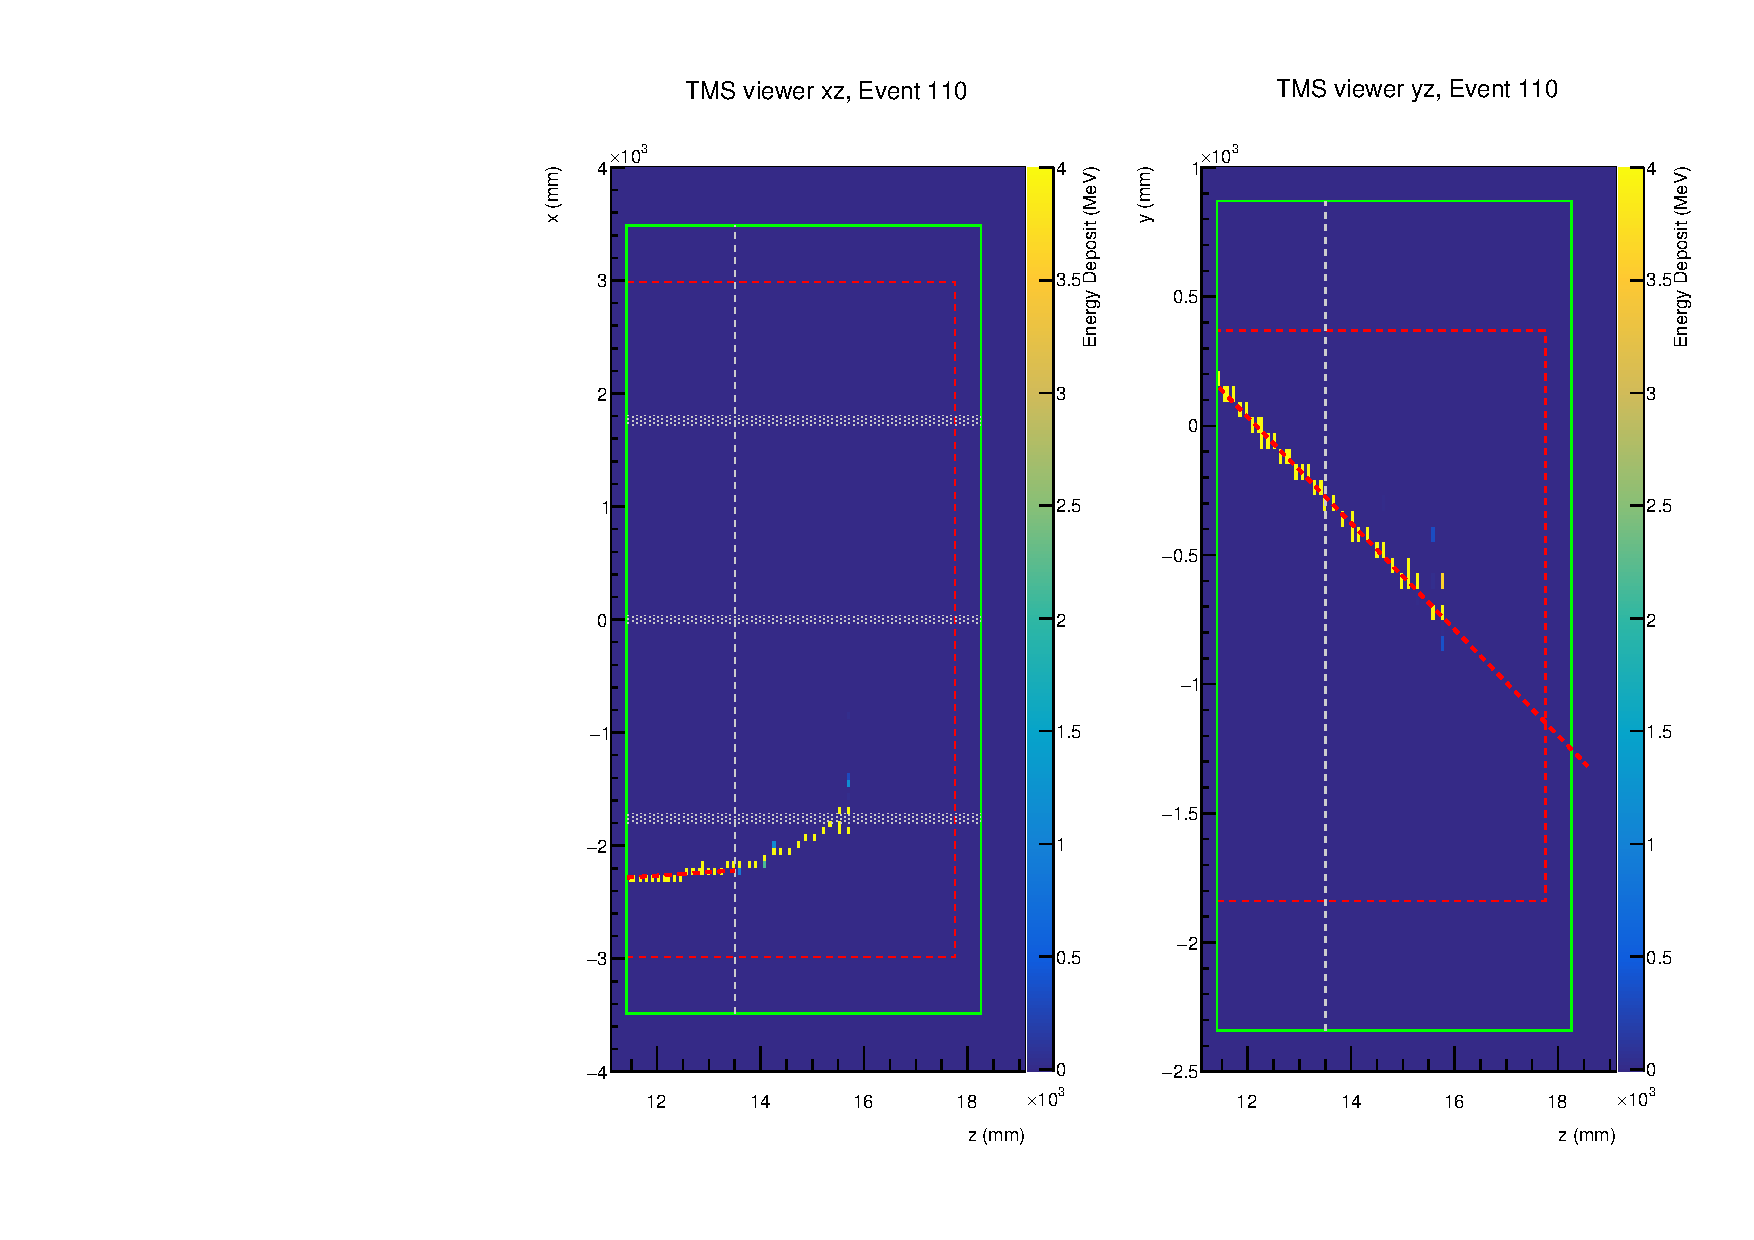
\includegraphics[width=0.49\textwidth]{graphics/Simulation/Hough/Hough_Example2.pdf}
\end{dunefigure}

An example of the A* track finding is shown in Figure \ref{fig:track_astar_1}, finding the optimal path between the last and first hit in $z$ separately in both views. It does so by choosing the path that minimises the cost related to connecting nearby cells, accounting for the change in distance from the goal cell. The implementation in \texttt{TMS\_Reco} allows switching A* to a greedy best-first search, where the distance to the goal cell is the only metric, and there is no cost incurred from connecting cells.
\begin{dunefigure}[]{fig:track_astar_1}
{Two single-track events in the TMS, where tracks are found by A* path-finding algorithm, showing $x-z$ (left) and $y-z$ (right) hits. The green and red boxes show the total and fiducial volume respectively, the vertical gray line shows the region where the TMS transitions from thin to thick iron layers, and the three horizontal white dotted regions in the $x-z$ view shows the gap region. The yellow fills show the hits that were found by the procedure. The right-most event has a clear secondary interaction, where the path bends abruptly in the $y-z$ view. N.B. the detector coordinate system differs from the event displays by being in mm (not cm) and translated by $\{x,y,z\}=\{0, 5, 411\}$ mm. }
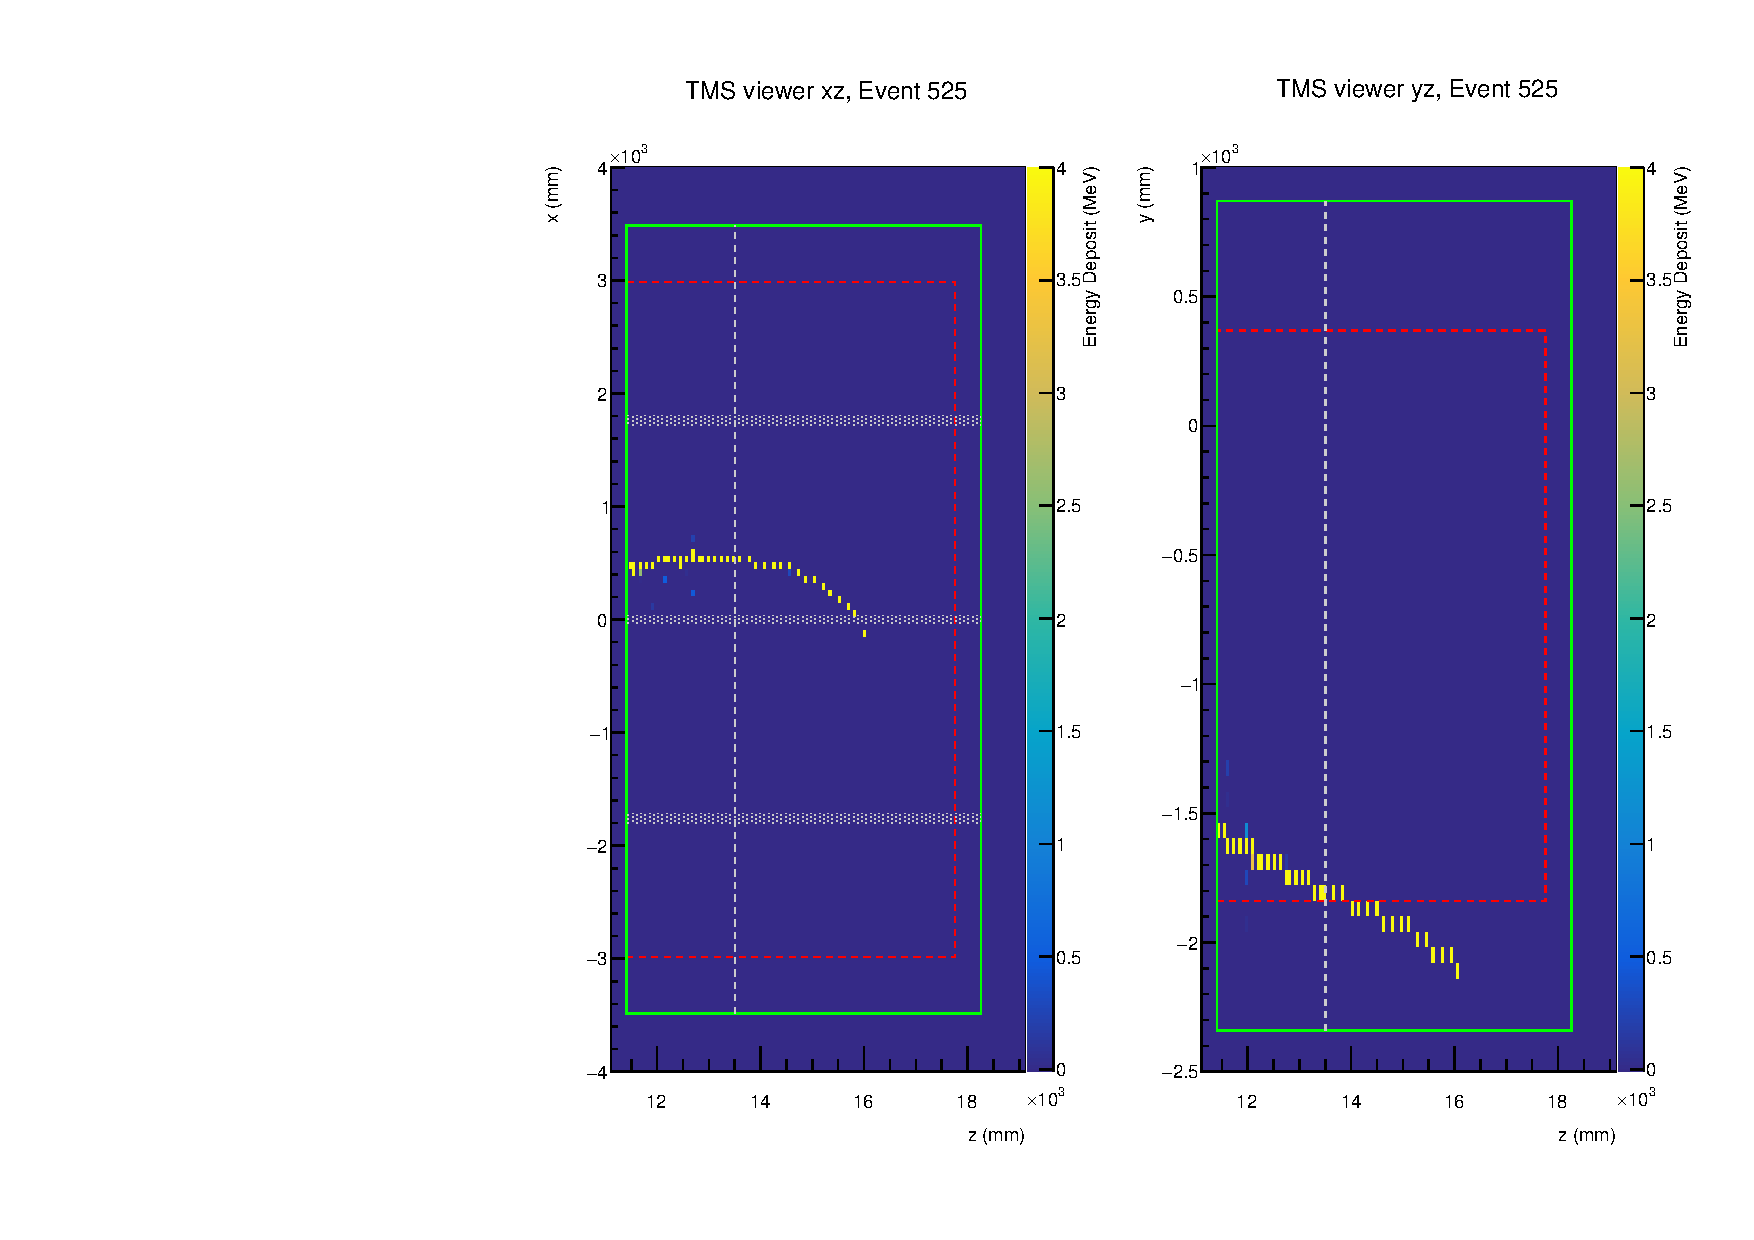
\includegraphics[width=0.49\textwidth]{graphics/Simulation/Astar/track_example_astar2.pdf} 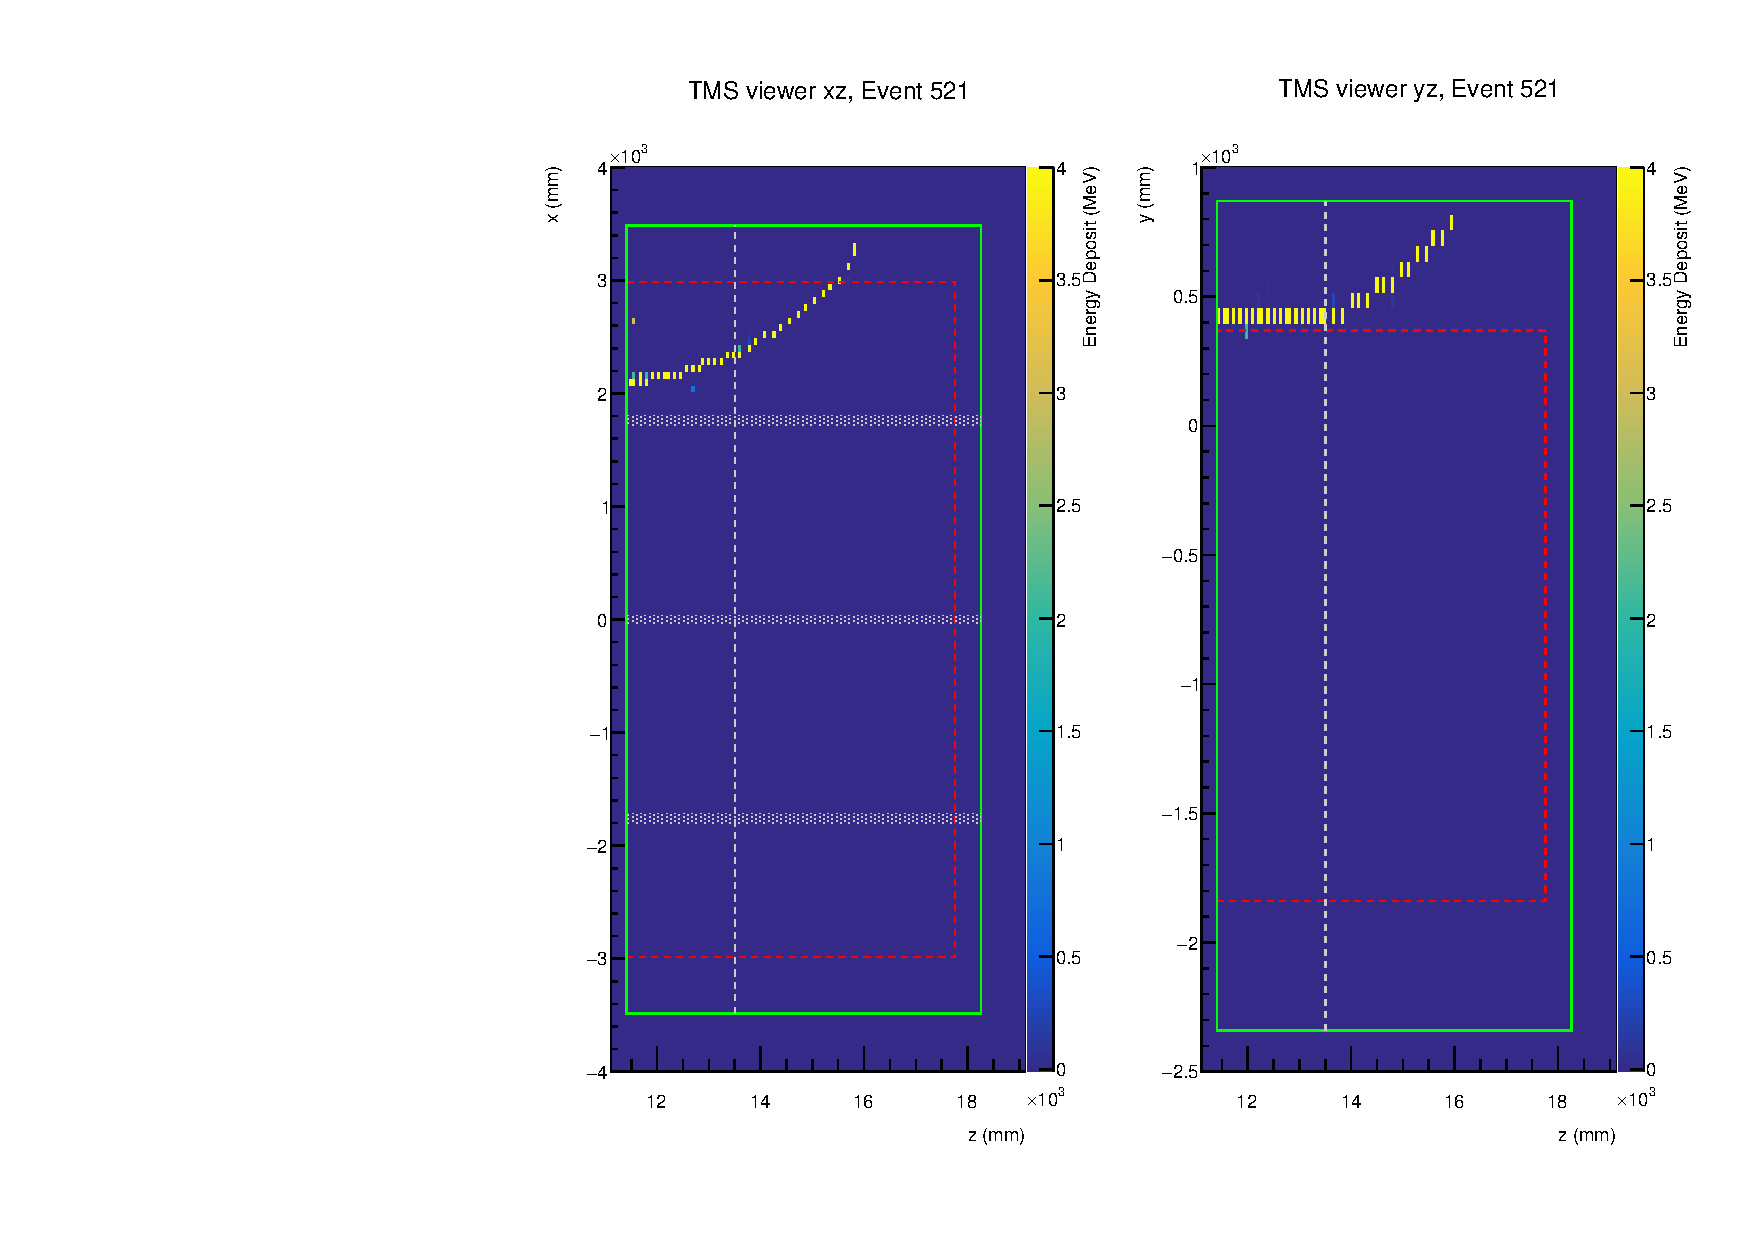
\includegraphics[width=0.49\textwidth]{graphics/Simulation/Astar/track_example_astar3.pdf}
\end{dunefigure}

\subsubsubsection{Track reconstruction}
\fixme{NEEDS EXPANDING AND IMPROVEMENTS!}
Lepton candidate is assumed to be the longest for the reconstruction stage. After reconstruction stage, lepton candidate is assumed to be the most energetic track that fits a muon hypothesis.

Combine 2D views in Kalman filter? Preliminary studies show track length is by far most important for a good KE measurement. Energy deposits along track length helps, and momentum estimate from bending is auxiliary. Run reconstruction stand-alone, and then with LAr seed? Back-propagate?

Stand-alone reconstruction without track seeding from the LAr will be possible. This could be used to provide a neutrino flux constraint on the TMS, or assisting with tracks in the SAND detector emanating upstream. This will be studied by generating neutrino interactions on the TMS volume.

\subsubsubsection{Integration with ArgonCube}
\fixme{Chris to write about LAr integration}

%%%%%%%%%%%%%%%%%%%%%%%%%%%%%%%%
\section{System Design}
\label{sec:tms-des}

%%%%%%%%%%%%%%%
\subsection{Transition Path to ND-GAr}
\label{sec:tms-des-path}

\fixme{Highlight this as unique feature}

A unique aspect of the \dword{tms}
is that it is temporary. It will operate for a few
years and then be replaced by the more capable 
\dword{ndgar}. This relaxes certain requirements,
for example the need to operate at a beam power of 2.4\,MW (something planned to happen beginning in year six) but imposes others, such as the need
to be removed with minimal impact to experiment
operations.

The replacement of the \dword{tms} by \dword{ndgar}, can be
accomplished in about two weeks. The procedure is
to build \dword{ndgar} on the west \dword{duneprism} rails. When
complete, temporary rail crossings between
the \dword{duneprism} east and west rails are installed,
the \dword{tms} is then disconnected and using these
rails moved from the west to east rails. From
there, \dword{tms} moves north on the west rails and
\dword{ndgar} south on the east rails. Then
\dword{ndgar} begins operation and TMS begins
disassembly.

During the \dword{ndgar} construction and \dword{tms} disassembly, the
\dword{duneprism} range of motion is reduced by about eight meters. It
would be possible to take additional running at the extreme
north position immediately before and after this period of restriction.

%%%%%%%%%%%%%%% One for each WBS element
%%%%%%%%%% The P6 WBS is not useful for this, as it breaks the work down
%%%%%%%%%%  by time, not activity
\subsection{Support Structure}
\label{sec:tms-des-structure}
The mechanical design consists of 2 parts, a steel support frame and a series of layered steel plates.  The support frame has four legs tied together with steel diagonal bracing. Bolted to the top of the legs are two beams W27 $\times$ 114,spaced \SI{6400}{\mm} apart. Transverse to those beams is a bed of five W30 $\times$ 191 beams evenly spaced. At the end of the transverse beams, bolted to the top, is a strong back consisting of two W8 $\times$ 24 beams tilted back at \SI{1.5}{\degree}. The bottom of the legs have heavy duty Hilman rollers to allow the frame to be moved using hydraulic cylinders.

The second part of the mechanical design is a series of \num{100} layered plates mounted to the bed of the steel support frame. The first \num{60} layers of plates are mounted on edge and lean against the strong back at \num{1.5} degrees. The plates are \SI{40}{\mm} steel and spaced \SI{40}{\mm} apart. The second \num{40} layers are \SI{15}{\mm} steel and spaced \SI{40}{\mm} apart. Each layer consists of three plates, two at \SI{1.75}{\m} nominal width and one at \SI{3.5}{\m} nominal width. All the plates are \SI{3.2}{\m} tall. There is a \SI{20}{\mm} gap between each of the plates. 
%To keep the plates from sliding, bolted to the W30 beams between each layer is a block \SI{38}{\mm} $\times$ \SI{25}{\mm} $\times$ \SI{177}{\mm}. 
%To maintain the \SI{40}{\mm} spacing and to anchor the plates, they are bolted together with spacer blocks in four equally spaced locations at the perimeter of the plates. The spacer blocks are drilled at a \num{1.5} degree angle and each bolt screws into the head of the previous bolt. 
At the sides of each plate is a notch, \SI{30}{\mm} $\times$ \SI{300}{\mm}, to receive the coils. The coils wrap around each of the three groups of plates.

%\begin{dunefigure}[Optional short caption for LoF]{fig:required-label}
%{Required full caption.}
%
\includegraphics[width=0.8\textwidth]{dunelogo_colorhoriz}
%\end{dunefigure}

An analysis was carried out to ensure that this support structure satisfies the AISC design provisions for the given loading conditions.  The analysis was performed with a combination of hand calculations and finite element modeling with SAP2000.  AISC 360-16 was be used as the guide for the strength design.  The design check calculates the design ratios for each member, taking into account all local member details, including lateral torsional buckling, local buckling effects depending on the member shapes, etc. as required by the AISC code, and determines which sections pass or fail the design check. Every structural member passes the design check based on the AISC design standards for combined axial loading and bi-axial bending.  The support structure was also checked for stability over tipover forces along the guided direction and the perpendicular direction for a nominal seismic force.   The assumed seismic force is found to be less than 90\% of the force required to cause tipover, indicating stability of the loaded structure against tipping.   
% some of Figures 6-8

%%%%%%%%%%%%%%%  One for each WBS element
\subsection{Detector Steel}
\label{sec:tms-des-steel}


% The coils cost us a bit less than 1% in acceptance.  T
The plates are made from the same 1006 steel used for  MINOS/BaBar which is high silicon, low-carbon, chosen for its magnetic properties ($\mu \ge 700$). 

The magnet has three design goals:
\begin{itemize}
    \item As high a field as possible inside the magnet,
    \item As uniform a field as possible inside the magnet,
    \item As low a field as possible outside the magnet.
\end{itemize}

These goals are somewhat in tension.

To reach these goals, each row of steel has two coil wraps to provide a uniform magnetic field.  Figure \cite{fig:tms_anl_coils} is a schematic of the coil and current flow.  There are two “belts” of coils in a “Helmholtzy” configuration which gives reasonably uniform field, especially between the coils.

The magnetic field configuration is approximately a dipole inside the steel, and a sextupole outside the steel.  This coil and field configuration strikes the balance between a large field inside the spectrometer, while keeping the field inside the \dword{arcube} as low as possible. 

\begin{dunefigure}[Schematic of coil arrangement and current flow]{fig:tms_anl_coils}
{Schematic of coil arrangement and current flow.}
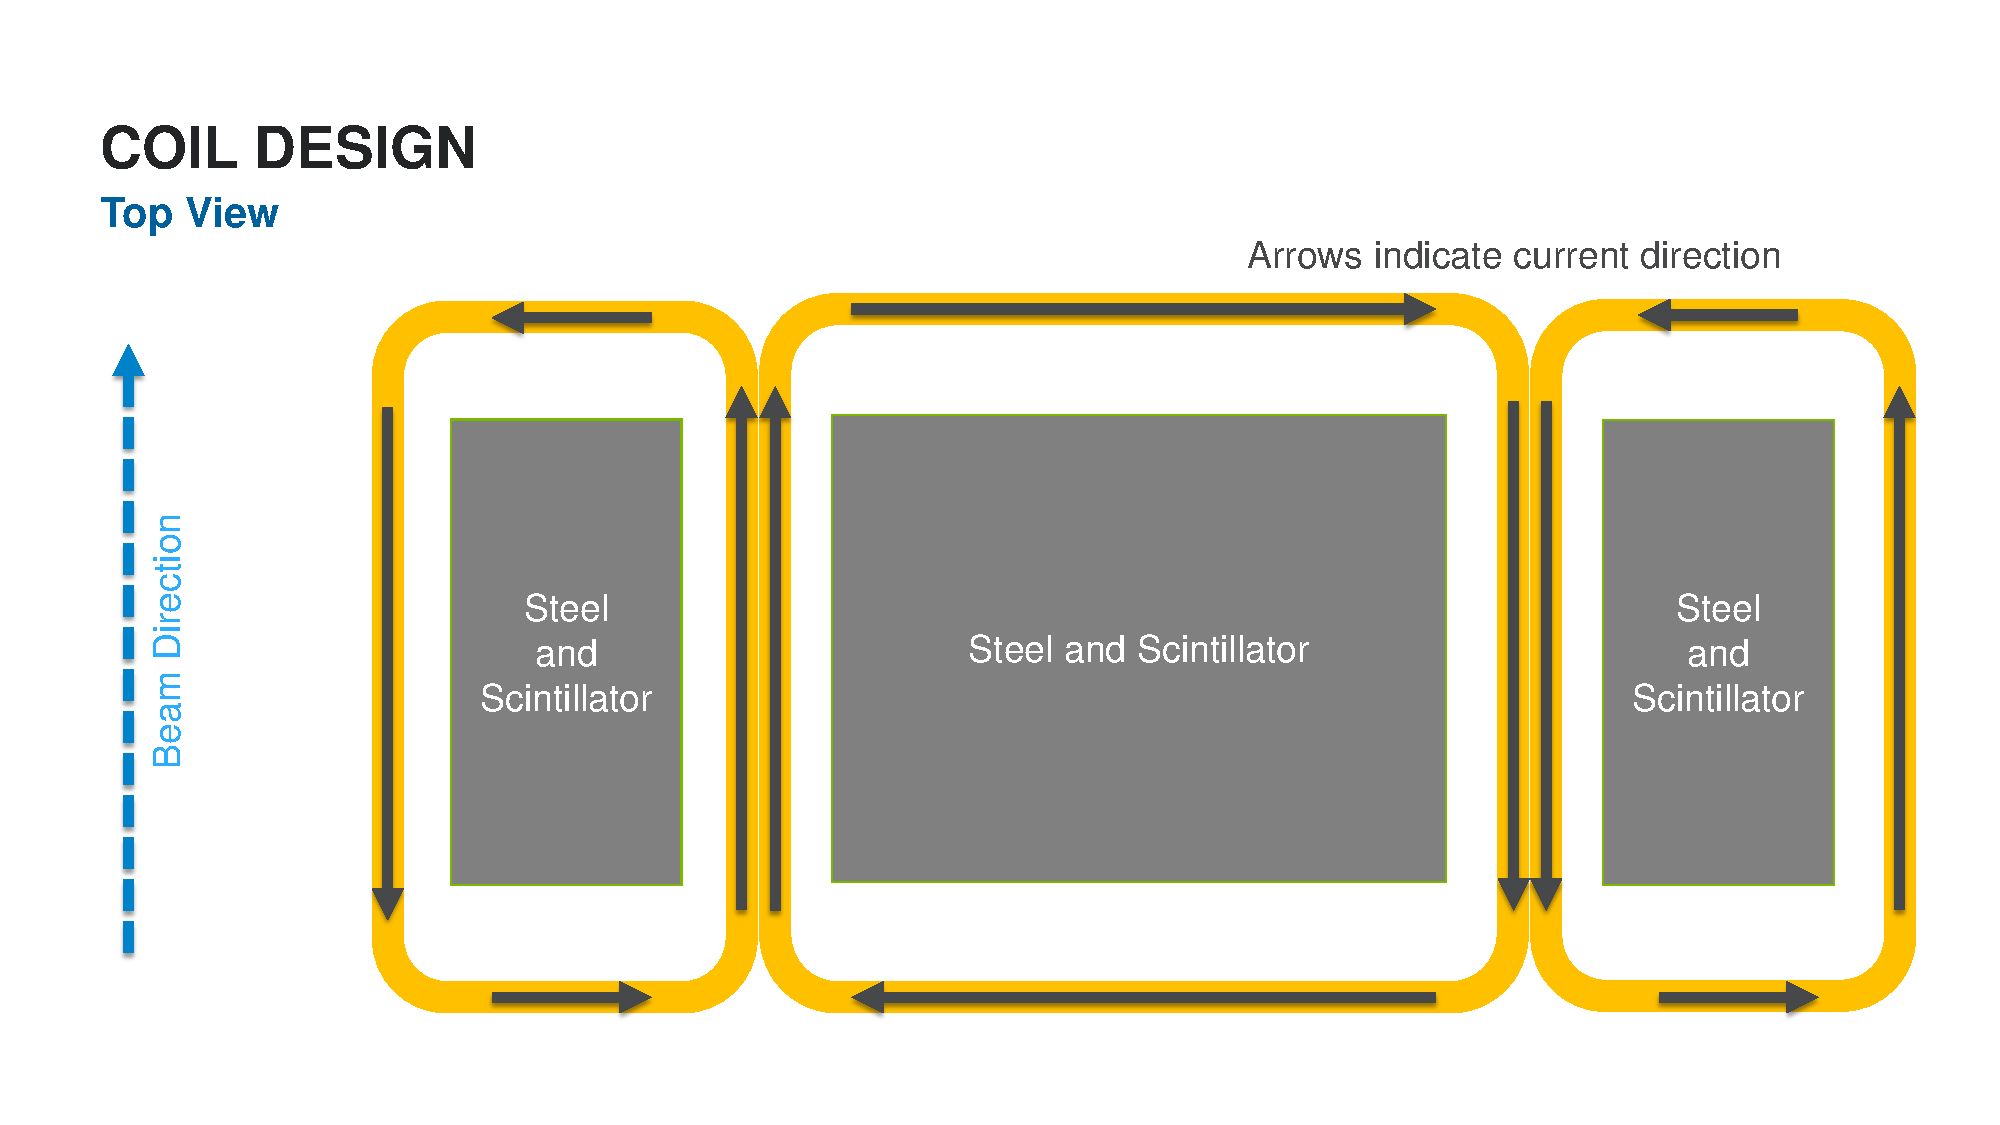
\includegraphics[width=0.8\textwidth]{graphics/Detector/tms_anl_coils.pdf}
\end{dunefigure}

%%%%%%%%%%%%%%%  One for each WBS element
\subsection{Magnet Coils and Power Supplies}
\label{sec:tms-des-coil}

 Figure \cite{fig:tms_anl_coils} is a schematic of the coil and current flow.  There are two “belts” of coils in a “Helmholtzy” configuration which gives reasonably uniform field, especially between the coils.  
The magnetic field configuration is approximately a dipole inside the coils, and a sextupole outside the coils, see Figure \cite{}.  

Additionally, there are cost considerations. There are 
tensions among the ensemble of goals. This design emphasizes
field magnitude, low fringe and low cost over field uniformity. The outer
two-quarters of the magnet have a field, nominally vertical, in the opposite
direction to the center half. Externally, these fields largely cancel: the
dipole component cancels; the quadrupole component largely cancels; and
the residual component is a sextupole.

A magnetic analysis was performed with the Low Frequency EMAG module in Ansys Multiphysics.   The goals of this analysis were to determine the magnetic field intensity and magnetic flux density in the spectrometer, determine the mechanical load due to the magnetic field on the plates, and determine the magnetic field adjacent to the spectrometer.   Each coil in the model consisted of two layers of \num{50} turns of \num{15} $\times$ \SI{10}{\mm} copper bar, giving a cross section of \num{30} $\times$ \SI{500}{\mm}.  The current in each turn was \num{150} A, for a total current of \num{15,000} A.  The current in each plate bundle flowed in a direction opposite that of the bundle next to it.  The model is a half symmetry, and was split on the global Y-Z plane. Solid geometry of the plates and air were created and then meshed with over four million SOLID96 eight node brick elements.   This model is shown in Figure \ref{fig:tms_anl_Bmodel1}.  Results of the magnetic field simulation are shown in Figure \ref{fig:tms_anl_Bfield1}.   In addition, the magnetic nodal forces were computed and found to be less than 25\% of the maximum pressure value.  
%Clarence put this in to make document compile
\iffalse
%This is shown Error! Reference source not found..  Boundary conditions (Figure 20) were flux-parallel on the symmetry plane and flux normal (MAG = 0) on the far field boundaries.  The flux normal boundary was achieved with INFINIT117 elements.

%The magnetic scaler potential formulation was used. 

%This method supports the use of a coil primitive, and bonded contact between regions in the model.  Due to the unusual range of dimensions in the geometry, these features were crucial to the development of a practical model.  The spectrometer consists of \num{100} thin (\num{20} and \SI{40}{\mm}thick) steel plates with a surface area of nearly \num{11} $m^2$ separated by \SI{40}{\mm} air gaps.  The coil bears directly on the steel plate, with only the insulation, estimated at \SI{1}{\mm} thick, between the copper conductor and the plate.  This four orders of magnitude between dimensions would be difficult to mesh as a single component, and the sheer size of the spectrometer would result in a very large element count.  
%Bonded contact with a magnetic degree of freedom and a coil primitive significantly streamlined the process.

%A model was built in Ansys MAPDL with a script.    The coil was modeled with SOURC36 current source primitive.  Symmetry cannot be applied to SOURC36 elements, so the whole coil is modeled. This model is shown in Figure 18 and the finite element mesh is shown in Figure 19.  
\fi

\begin{dunefigure}[ANSYS model used for the magnetic field simulation.]{fig:tms_anl_Bmodel1}
{ANSYS model used for the magnetic field simulation.  Left:  Solid geometry for the magnetic simulation.  Right:  Finite Element Mesh used in the magnetic field simulation.   }
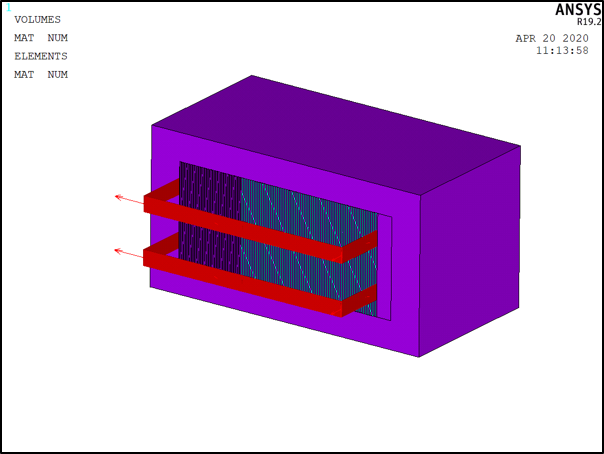
\includegraphics[width=0.49\textwidth]{graphics/Detector/tms_anl_Bmodel1.pdf} 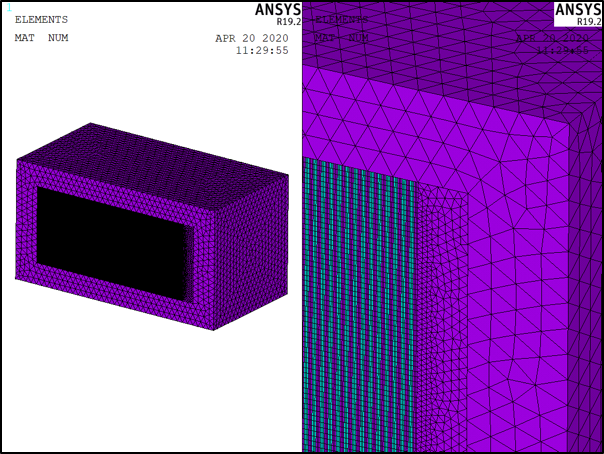
\includegraphics[width=0.49\textwidth]{graphics/Detector/tms_anl_Bmodel2.pdf}
\end{dunefigure}

\begin{dunefigure}[ANSYS model used for the magnetic field simulation.]{fig:tms_anl_Bfield1}
{Results of the magnetic field simulation.   Left:  Magnetic flux density (T), \SI{40}{\mm} plates in front.  Right:  Magnetic flux density beyond last \SI{40}{\mm}  plate. }
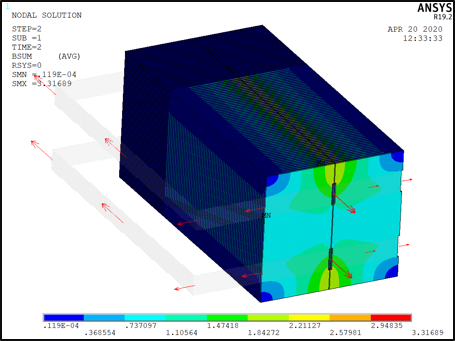
\includegraphics[width=0.49\textwidth]{graphics/Detector/tms_anl_Bfield1.pdf} 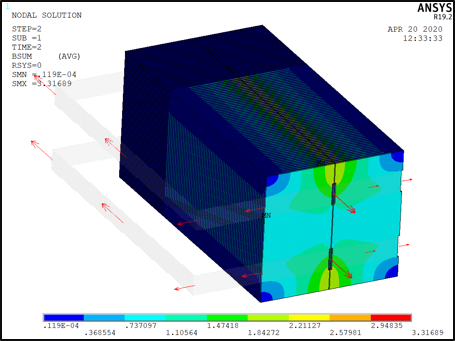
\includegraphics[width=0.49\textwidth]{graphics/Detector/tms_anl_Bfield1.pdf}
\end{dunefigure}

%%%%%%%%%%%%%%%  One for each WBS element
\subsection{Detector Modules}
\label{sec:tms-des-panels}

The \dword{tms} will have \num{400} modules each consisting of a single layer of plastic scintillator glued between \num{2} sheets of aluminum.  Each module will include \num{48} - \SI{3.5}{\cm} wide $\times$ \SI{1}{\cm} thick $\times$ \SI{300}{\cm} long scintillators.  Each scintillator is outfitted with a single WLS fiber threaded through a hole centered in the scintillator and extending the full length.  

The dword{wls} fibers exiting the scintillators will be divided into three groups of \num{16} and routed in a fiber trayto three separate fiber guide bars (FGB).  The ends of \dword{wls} fibers are precisely located by the FGB.  A manifold housing a 4x4 array of \dword{sipm} and a counter motherboard can then be mounted to each of the three FGBs for readout.  The module manifold is shown in Figure \ref{fig:tms_anl_module}.  

\begin{dunefigure}[Module Manifold Layout]{fig:tms_anl_module}
{Module manifold layout.}
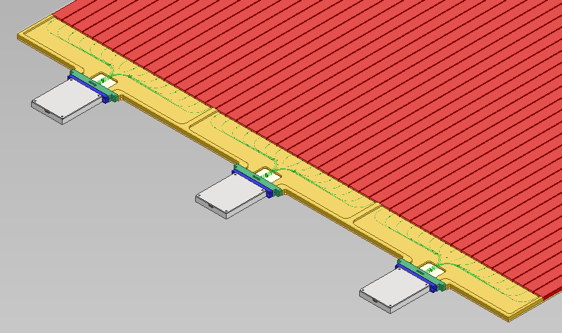
\includegraphics[width=0.6\textwidth]{graphics/Detector/tms_anl_module.pdf}
\end{dunefigure}

%%%%%%%%%%%%%%%  One for each WBS element
\subsection{Detector Electronics}
\label{sec:tms-des-electronics}
\subsubsection{On-Panel Boards}
\label{sec:tms-des-elect-OPB}

\fixme{notice the dwords and '\threed'. Do you want  OPB, SBC glossary items? (Anne)}
\fixme{I consider myself suitably chastised. I am saddened and maybe even ashamed that I missed a DUNEword or two (Tom)}

The wavelength-shifting fibers are attached to the
16-channel \dword{sipm} (Hamamatsu S13361-2050AE-04) via a 
\threed printed custom connector and light diffuser. This is mounted on 
one of the two electronics subsystems, the On-Panel Board (OPM).

From the \dword{sipm}, the signals are amplified by an 8$\times$ preamp,
and from there to the Analog Front-End/\dshort{adc} chip. We
have tentatively selected the eight-channel Texas Instrument AFE5807\footnote{Texas Instrument\texttrademark{} AFE5807, \url{https://www.ti.com/product/AFE5807}}.
This chip digitizes at 80\,MSPS and outputs \dword{lvds}.

Forget it. Edit it and I'll come back later.

Thee \dword{lvds} signals are sent via 50 pair/100 conductor cable
to the data concentrators.

\subsubsection{Data Concentrators}
\label{sec:tms-des-elect-DC}

There are eight data concentrators, each servicing fifty
panels or 2400 channels. Their job is to mate the
 \dword{lvds}  signals from the OPBs to the \dword{daq}. Each contains
a \dword{fpga} to do the fast processing and a small single-board
computer (SBC) to send this data over Ethernet as 
TCP/IP packets or \dword{udp} datagrams. Each packet will
contain the channel number, the event time, and the channel
energy.



%%%%%%%%%%%%%%%  One for each WBS element
\subsection{Installation, Transport and Assembly}
\label{sec:tms-des-transport}

\fixme{Do we want this here or in the later section?}

%%%%%%%%%%%%%%%%%%%%%%%%%%%%%%%%
\section{Interfaces}
\label{sec:tms-interface}

Table~\ref{tbl:larndinterfaces} contains a summary and brief description of all the interfaces between the \dword{tms} consortium and other consortia, working groups, and task forces, with references to the current version of the interface documents describing those interfaces.  
Drawings of the mechanical interfaces and diagrams of the electrical interfaces are 
included in the interface documents as appropriate.
It is expected that further refinements of the interface documents will take place prior to the final \dword{prr} for the detector. The interface documents specify the responsibility of different consortia or groups during all phases of the experiment including design and prototyping, integration,  installation, and  commissioning.


\begin{dunetable}
[\dshort{tms} interface links]
{p{0.25\textwidth}p{0.5\textwidth}l}
{tbl:larndinterfaces}
{\dshort{tms} interface links}
Interfacing System & Description & Linked Reference \\ \toprowrule
Cryostat      &  (desc)
& \citedocdb{?} \\ \colhline

\dshort{duneprism} &  (desc)
& \citedocdb{?} \\ \colhline

\dshort{sand}  &  (desc)
& \citedocdb{?} \\ \colhline

Computing  &  (desc)
& \citedocdb{?} \\ \colhline

\dshort{daq}    &  (desc)
& \citedocdb{?} \\
\end{dunetable}



%%%%%%%%%%%%%%%%%%%%%%%%%%%%%%%%
\section{Risks and Mitigations}
\label{sec:tms-risks}

Table~\ref{tab:risks:ND-LAr} contains a list of all the
risks that \dword{dune} is currently holding in the \dword{tms} risk register.  Each line includes the official \dword{dune} risk register identification number, a description of the risk, the proposed mitigation for the risk, and finally three columns rating the post-mitigation (P)robability that the risk described comes to pass, the degree of (C)ost risk for that line, and the degree of (S)chedule risk.  Risk levels are defined as (L)ow (<10\% probability of occurring, <5\% cost impact, <2 month schedule impact), (M)edium (10 to 25\% probability of occurring, 5\% to 20\% cost impact, 2 to 6 month schedule impact), or (H)igh (>25\% probability of occurring, >20\% cost impact, >6 month schedule impact).  Most of these risks are reduced to a ``Low'' level following mitigation (as shown in the table), although several of them currently hold a higher risk levels (pre-mitigation), due to the early stage of development of the \dword{tms} system relative to other systems.  

In the following sections, we present a narrative description of each of the risks and the proposed mitigation.

\fixme{Anne needs to get risk table template put together}


\begin{itemize}
\item Trapped modules 
\item Calibration (no light injection system)?
\end{itemize}

%\input{generated/risks-longtable-ND-LAr.tex}

\begin{dunetable}
[Placeholder for risks table]
{cc}
{tab:table-tms-risks}
{Placeholder for Risks Table - it will be generated from a spreadsheet}
Rows & Counts \\ \toprowrule
Row 1 & First \\ \colhline
Row 2 & Second \\ \colhline
Row 3 & Third \\ % no \colhline on final row
\end{dunetable}

%%%%%%%%%%%%%%%%%%%%%%%%%%%%%%%%
\section{Schedule}
\label{sec:tms-org-sched}

Table \ref{tab:tms-sched} lists key milestones in the design, validation, construction, and installation of the \dword{tms}.  These milestones include external milestones indicating linkages to the main \dword{dune} schedule (highlighted in color in the table), as well as internal milestones such as design validation and technical reviews.

\fixme{Anne to get list of main DUNE sched items from Eric J before making the real table template}


\begin{itemize}
\item Finalize magnet design
\item Finalize module design
\end{itemize}
 

\begin{longtable}
{p{0.75\textwidth}p{0.25\textwidth}}
\caption{\dshort{tms} consortium schedule}\\ \colhline
\rowcolor{dunetablecolor}Milestone & Date   \\ \toprowrule


\rowcolor{dunepeach}Beneficial occupancy of cavern 1 and \dword{cuc}& \cucbenocc      \\ \colhline
Initial batch (80 PD modules) assembled  & March 2023\\ \colhline

\rowcolor{dunepeach}Top of \dword{detmodule} \#1 cryostat accessible& \accesstopfirstcryo      \\ \colhline
Third batch (320 PD modules) arrive at US PD Reception Facility  & January 2024\\ 

\label{tab:tms-sched}
\end{longtable}

%%%%%%%%%%%%%%%%%%%%%%%%%%%%%%%%
\section{Prototyping Plans}
\label{sec:tms-proto}

\fixme{Hugh to add material on Tufts efforts, Mat on cable testing at Wichita State.} 
\begin{itemize}
\item SiPM/fiber connection
\item Design of SiPM/Electronics board 
\item cable testing 
\end{itemize}

%%%%%%%%%%%%%%%%%%%%%%%%%%%%%%%%
\section{Construction Plans}
\label{sec:tms-construc}

\fixme{ Hugh and Tom }
\begin{itemize}
\item Support / steel assembly 
\item Coil assembly 
\item Module assembly - refs. To MINOS / mu2e. (several Figures from 36-41)
\end{itemize}

%%%%%%%%%%%%%%%%%%%%%%%%%%%%%%%%%%%%%%%%%%%%%%%%%%%%%%%%%%%%%%%% 
\begin{comment} % comment here to end
\fixme{The following sections are not in the new structure; I'm keeping them at the end here for now, in case you want to include one or more of them later.}

%%%%%%%%%%%%%%%%%%%%%%%%%%%%%%%% Not in Tim's new organization
\section{Safety Concerns}
\label{sec:tms-safety}


%%%%%%%%%%%%%%%%%%%%%%%%%%%%%%%% Not in Tim's new organization
\section{Calibration}
\label{sec:tms-calib}

%%%%%%%%%%%%%%%%%%%%%%%%%%%%%%%% Not in Tim's new organization
\section{Quality Assurance}
\label{sec:tms-qa}

%%%%%%%%%%%%%%%%%%%%%%%%%%%%%%%% Not in Tim's new organization
\section{Production, Assembly, and Quality Control}
\label{sec:tms-qc}

%%%%%%%%%%%%%%%%%%%%%%%%%%%%%%%% Not in Tim's new organization
\section{Transport and Handling}
\label{sec:tms-transport}

%%%%%%%%%%%%%%%%%%%%%%%%%%%%%%%% Not in Tim's new organization
\section{Installation, Integration, and Commissioning}
\label{sec:tms-iic}

%%%%%%%%%%%%%%%%%%%%%%%%%%%%%%%% Not in Tim's new organization
\section{Organization}
\label{sec:tms-org}

%%%%%%%%%%%%%%% Not in Tim's new organization
\subsection{Participating Institutions}
\label{sec:fdsp-org-inst}
%\metainfo{\color{red}\bf  Content: Segreto/Warner}

The \dword{tms} consortium benefits from the contributions of many institutions and facilities in \fixme{several countries? or the U.S. and ??}.  Table~\ref{tab:tms-institutes}
lists the member institutions. 

\begin{longtable}
{ll}
\caption{\dshort{tms} consortium institutions}\\ \colhline
\rowcolor{dunetablecolor} Member Institute  &  Country       \\  \toprowrule
univ 1 &  \\ \colhline
univ 2 &  \\ \colhline
univ 3 &  \\ 
\label{tab:tms-institutes}
\end{longtable}


\end{comment}









